\documentclass[fleqn,10pt]{wlscirep}
\usepackage[utf8]{inputenc}
\usepackage[T1]{fontenc}
\usepackage{makecell}

\title{Supplementary Information}


\author[1,2,*,\textsuperscript{\textdagger}]{Carmen Cabrera}
\author[3]{Miguel González-Leonardo}
\author[1]{Andrea Nasuto}
\author[2]{Ruth Neville}
\author[1,\textsuperscript{\textdagger}]{Francisco Rowe}
\affil[1]{Geographic Data Science Lab, Department of Geography and Planning, University of Liverpool, Liverpool, UK}
\affil[2]{Centre for Advanced Spatial Analysis, University College London, London, UK}
\affil[3]{Centre for Demographic Urban and Environmental Studies, El Colegio de México, México City, México}


\affil[*]{Corresponding author: c.cabrera@liverpool.ac.uk}

\affil[ \textsuperscript{\textdagger}]{These authors have contributed equally to this study.}


%\keywords{Keyword1, Keyword2, Keyword3}


\begin{abstract}
Urban mobility is central to economic activity, social inclusion and access to services. COVID-19 caused disruptions to mobility globally, yet its long-term impacts in less developed countries remain poorly understood. Using an unprecedentedly large dataset of >170 million mobile phone records from Meta-Facebook users in Argentina, Chile, and Colombia (March 2020–May 2022), we find sustained changes in mobility across socioeconomic and rural–urban gradients. We reveal that mobility recorded the sharpest declines and remained below pre-pandemic levels in most high-density and low socio-economic deprivation areas, while low-density and more deprived communities returned to baseline. These differences reflect the scale of the initial mobility shock, rather than subsequent recovery rates. Our findings reveal how a global shock can entrench disparities in human mobility, with implications for economic resilience, social inclusion and urban planning in unequal nations. Our study underscores the need for proactive policies to prevent long‑lasting inequalities in mobility.


\end{abstract}

\begin{document}

\flushbottom

\maketitle
% * <john.hammersley@gmail.com> 2015-02-09T12:07:31.197Z:
%
%  Click the title above to edit the author information and abstract
%

% * <john.hammersley@gmail.com> 2015-02-09T12:07:31.197Z:
%
%  Click the title above to edit the author information and abstract

\section{Processing Facebook data}

\subsection{Missing values}

\begin{table}[h!]
\centering
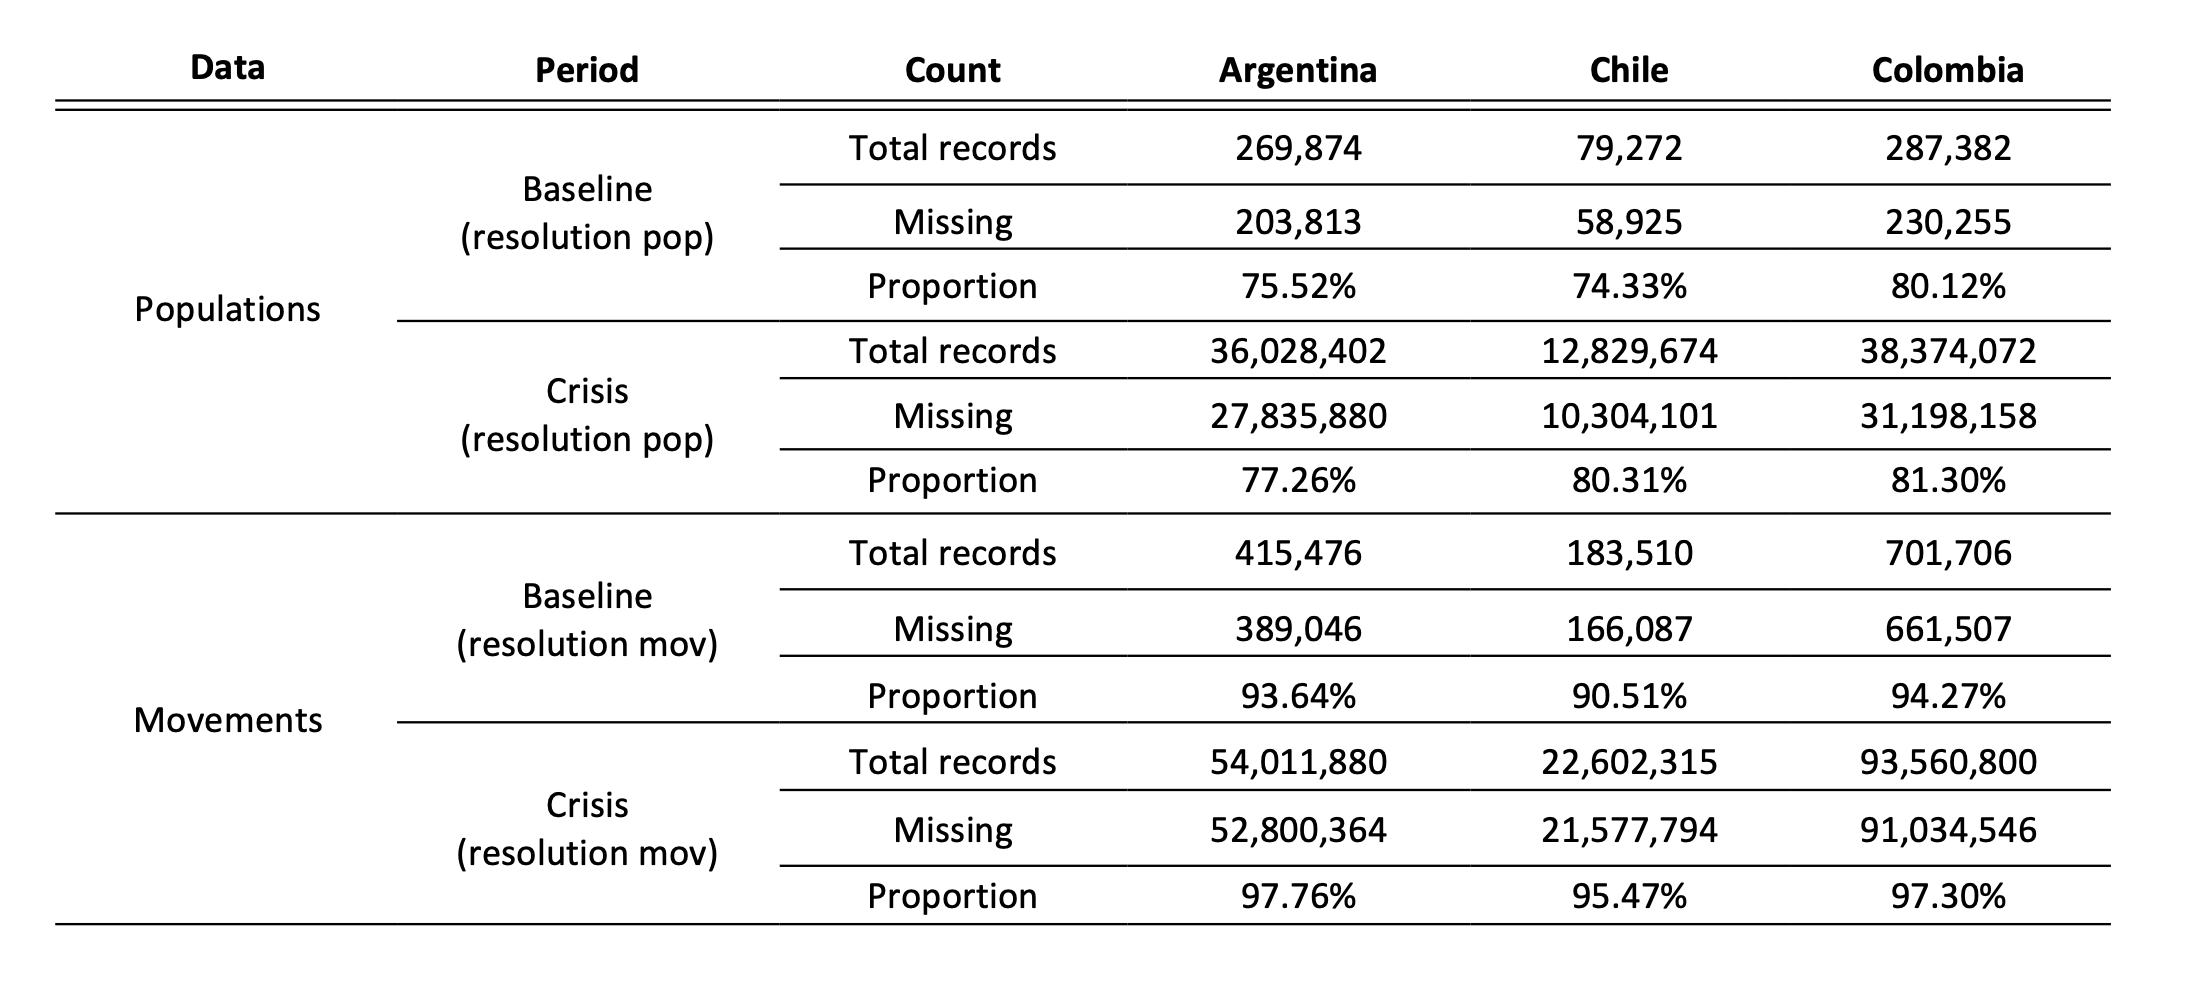
\includegraphics[width=\linewidth]{supplementary/missing/SF-missing-data-table.png}
\caption{Proportion of missing values for Facebook Population and Facebook Movements data, during baseline and crisis in Argentina, Chile and Colombia.}
\end{table}

\newpage

\begin{figure}[h!]
\centering
\includegraphics[width=.7\linewidth]{supplementary/missing/SF-missing.png}
\caption{Facebook Population baseline records corresponding to Monday, for Argentina, Chile and Colombia. The first row shows the original records, which include a high proportion of missing values. The second row shows the imputed baseline following a regression model with Worldpop data.}
\label{missing-baseline}
\end{figure}

\newpage

\subsection{Relationship between WorldPop population and Facebook Population baseline data for each day of the week}

\begin{figure}[h!]
\centering
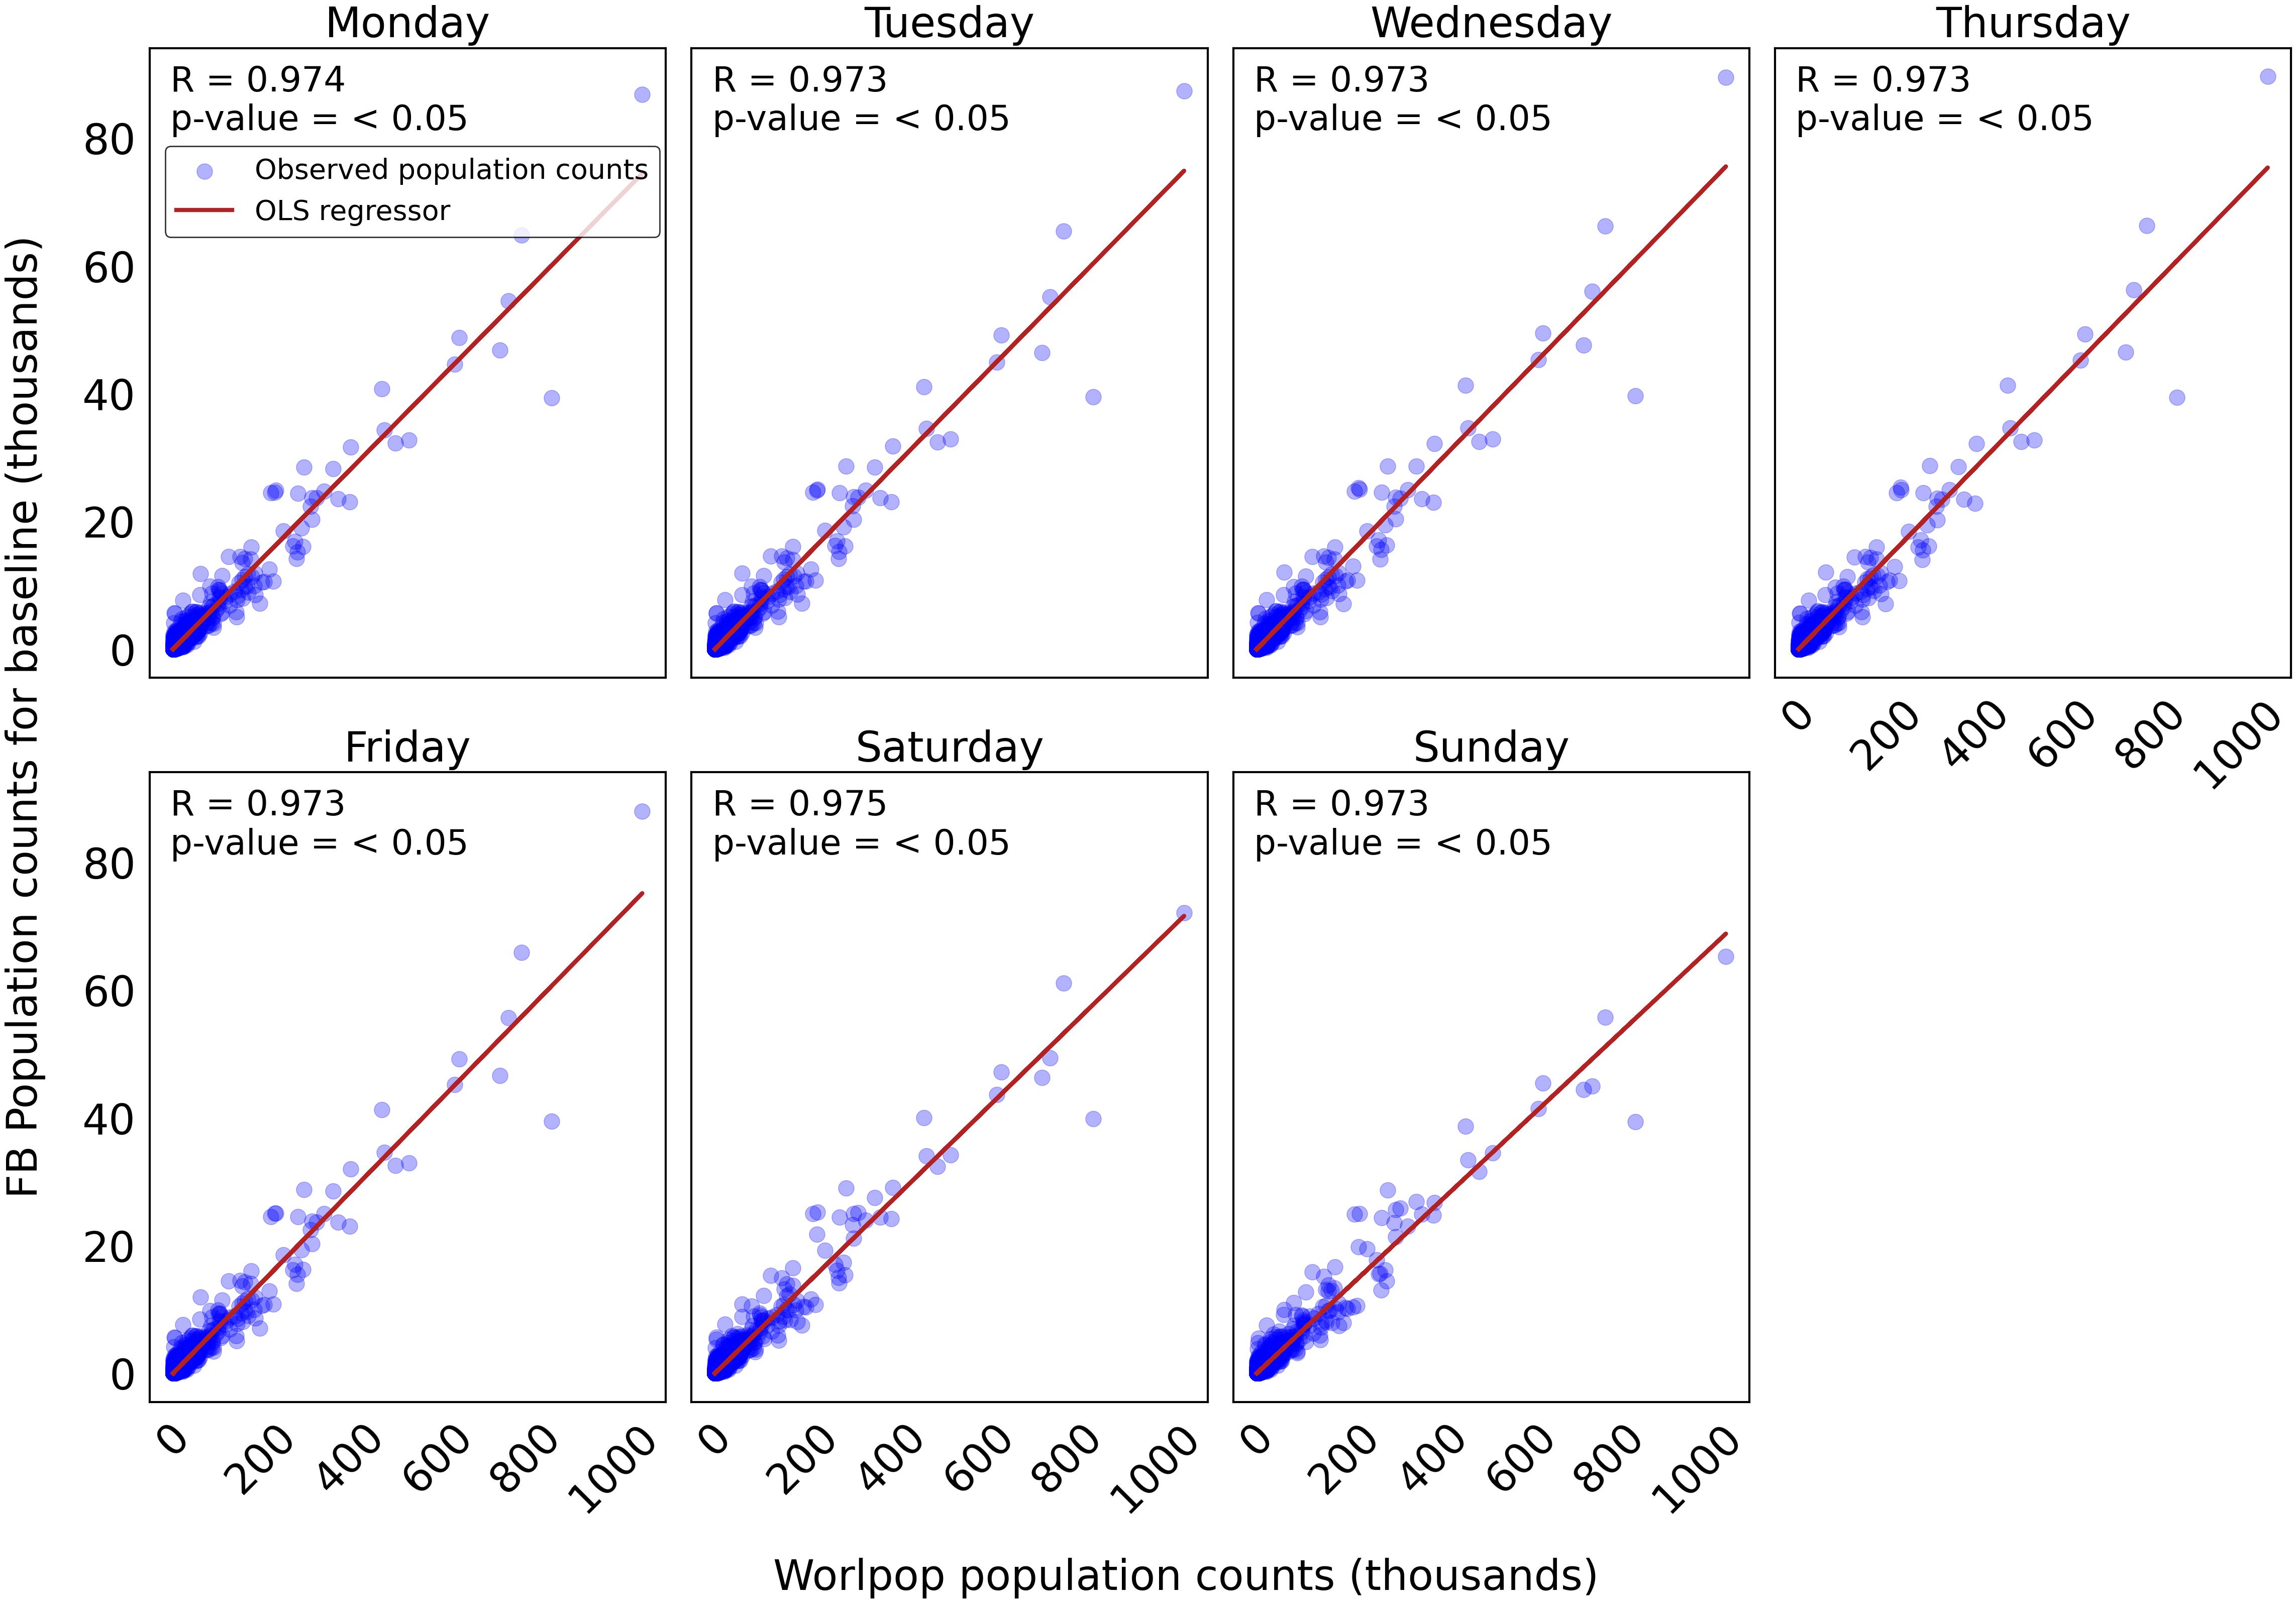
\includegraphics[width=\linewidth]{supplementary/correlation/correlation-wp-fb-pop-baseline-ARG.png}
\caption{Correlation between Worldpop population counts and Facebook Population counts during the baseline period in Argentina, for each day of the week.}
\label{correlation-wp-fbpop-ARG}
\end{figure}

\newpage

\begin{figure}[h!]
\centering
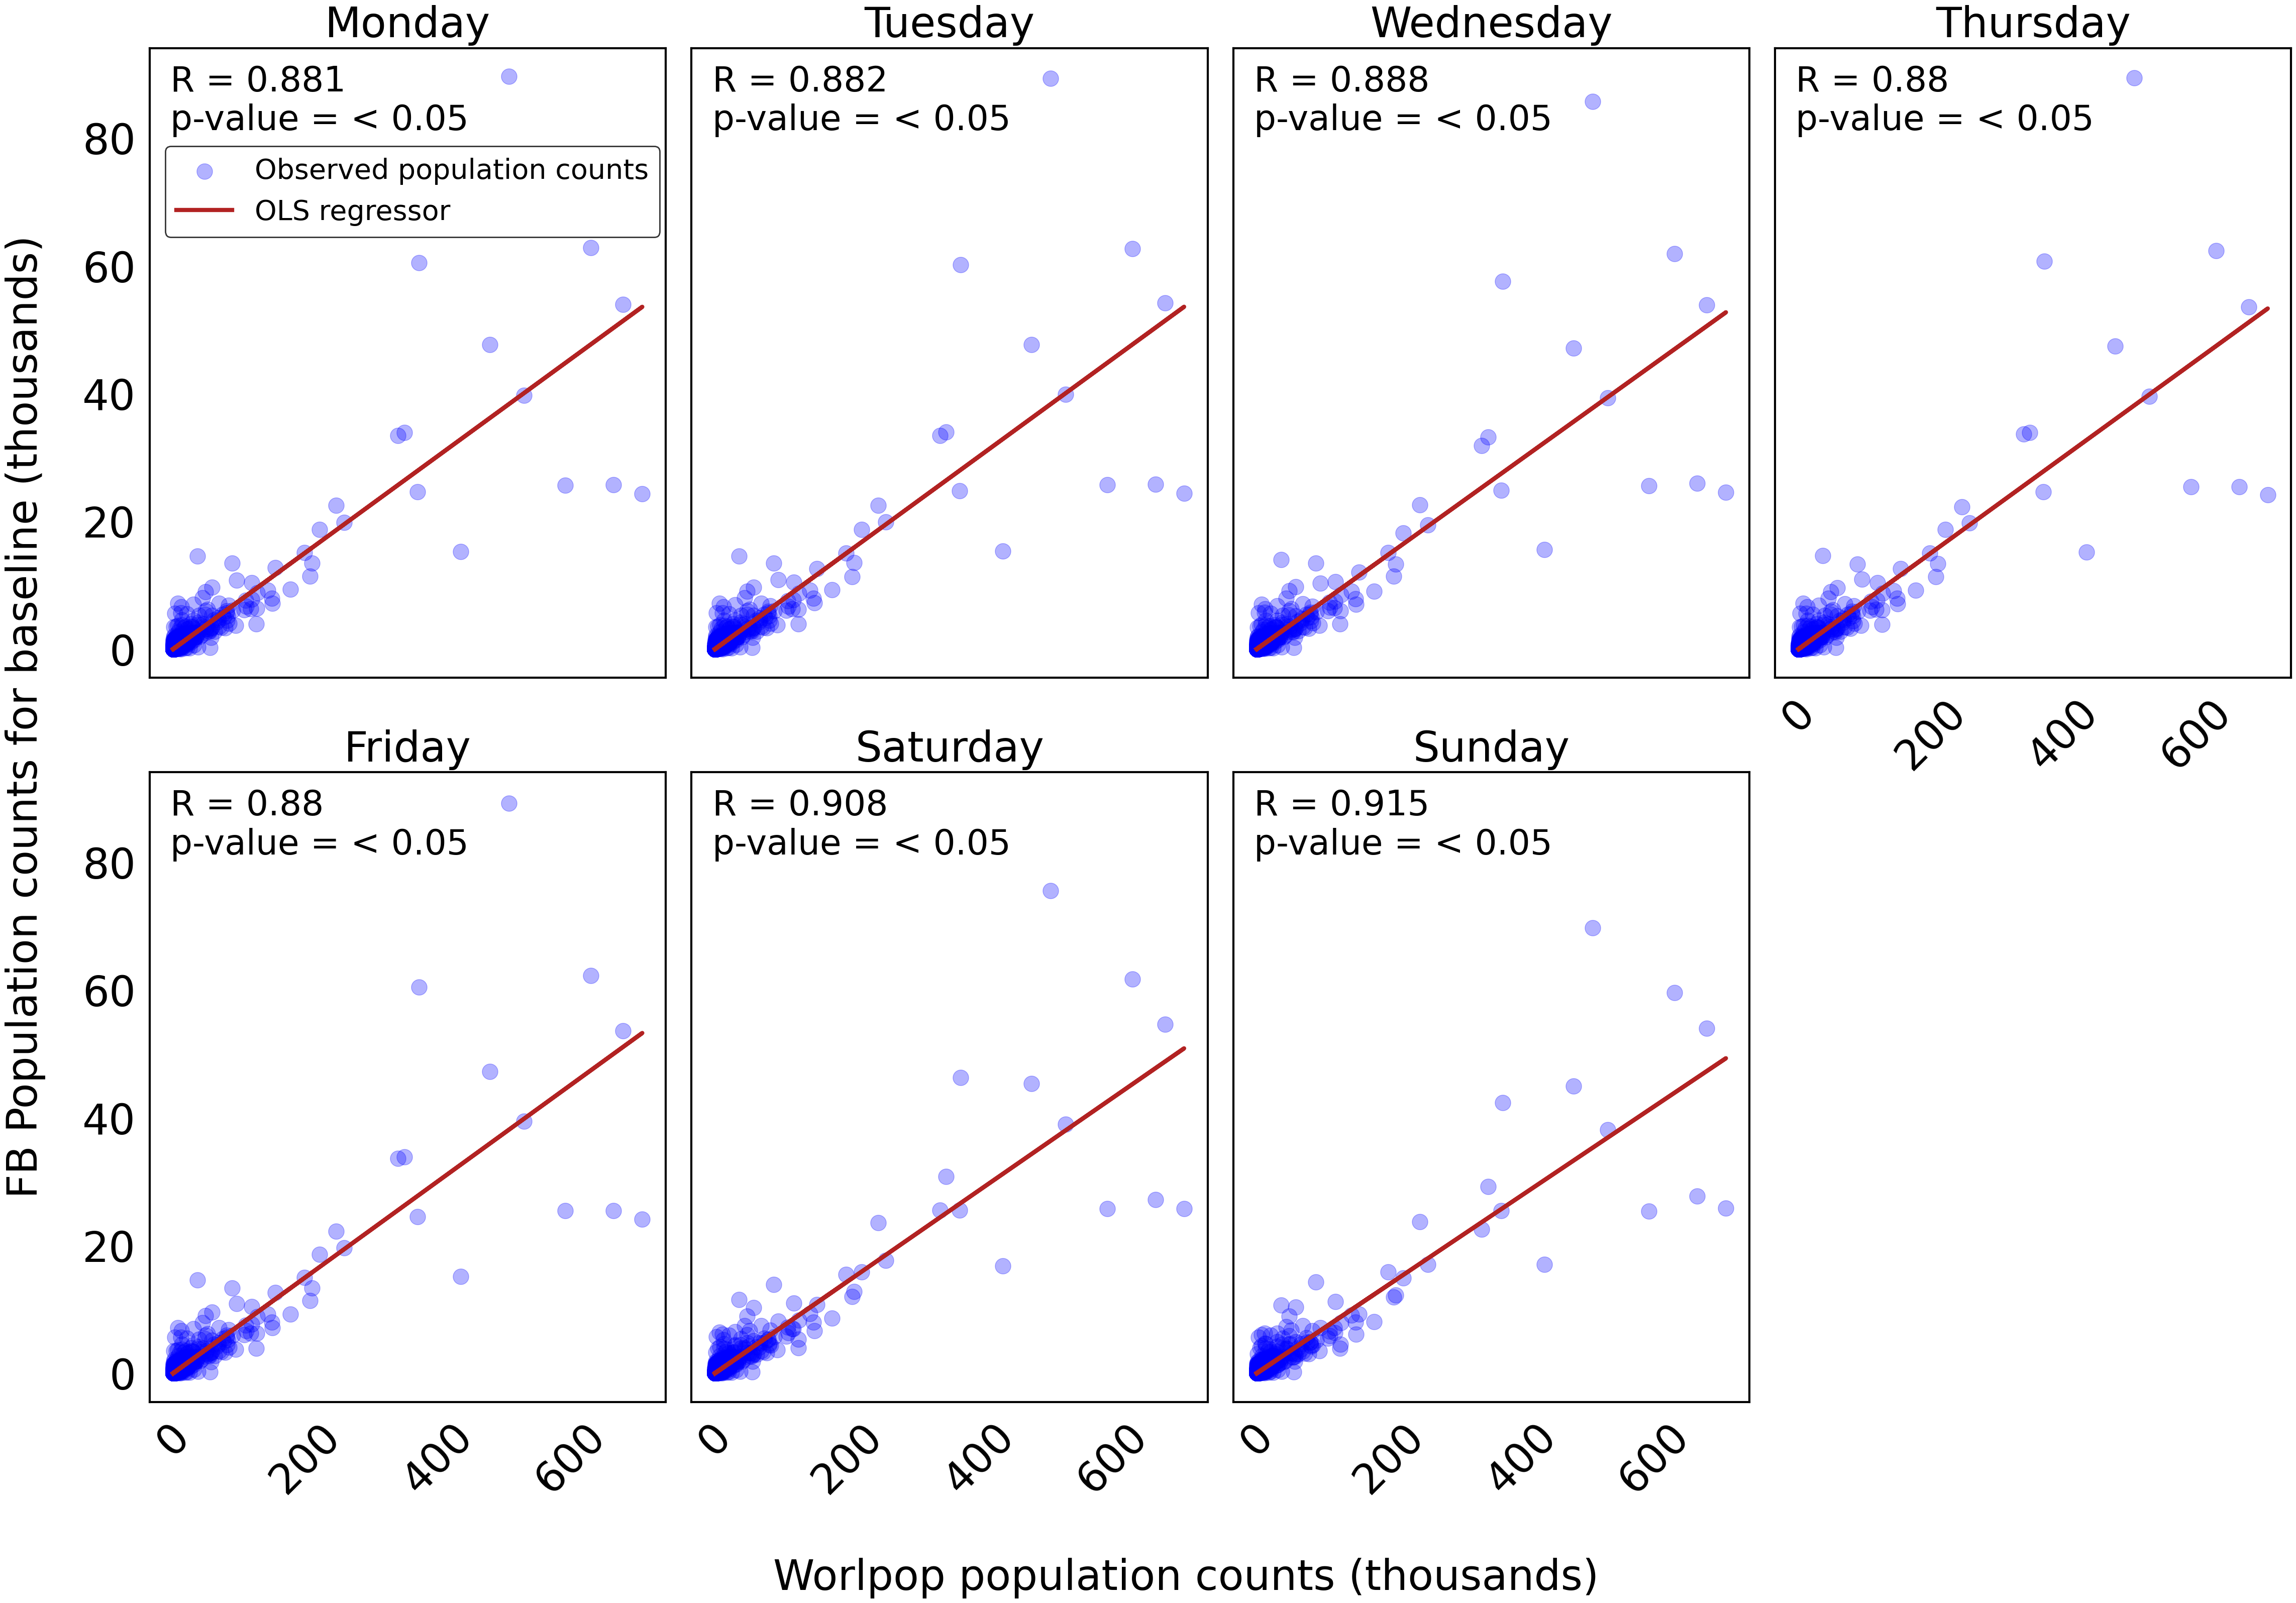
\includegraphics[width=\linewidth]{supplementary/correlation/correlation-wp-fb-pop-baseline-CHL.png}
\caption{Correlation between Worldpop population counts and Facebook Population counts during the baseline period in Chile, for each day of the week.}
\label{correlation-wp-fbpop-CHL}
\end{figure}

\newpage

\begin{figure}[h!]
\centering
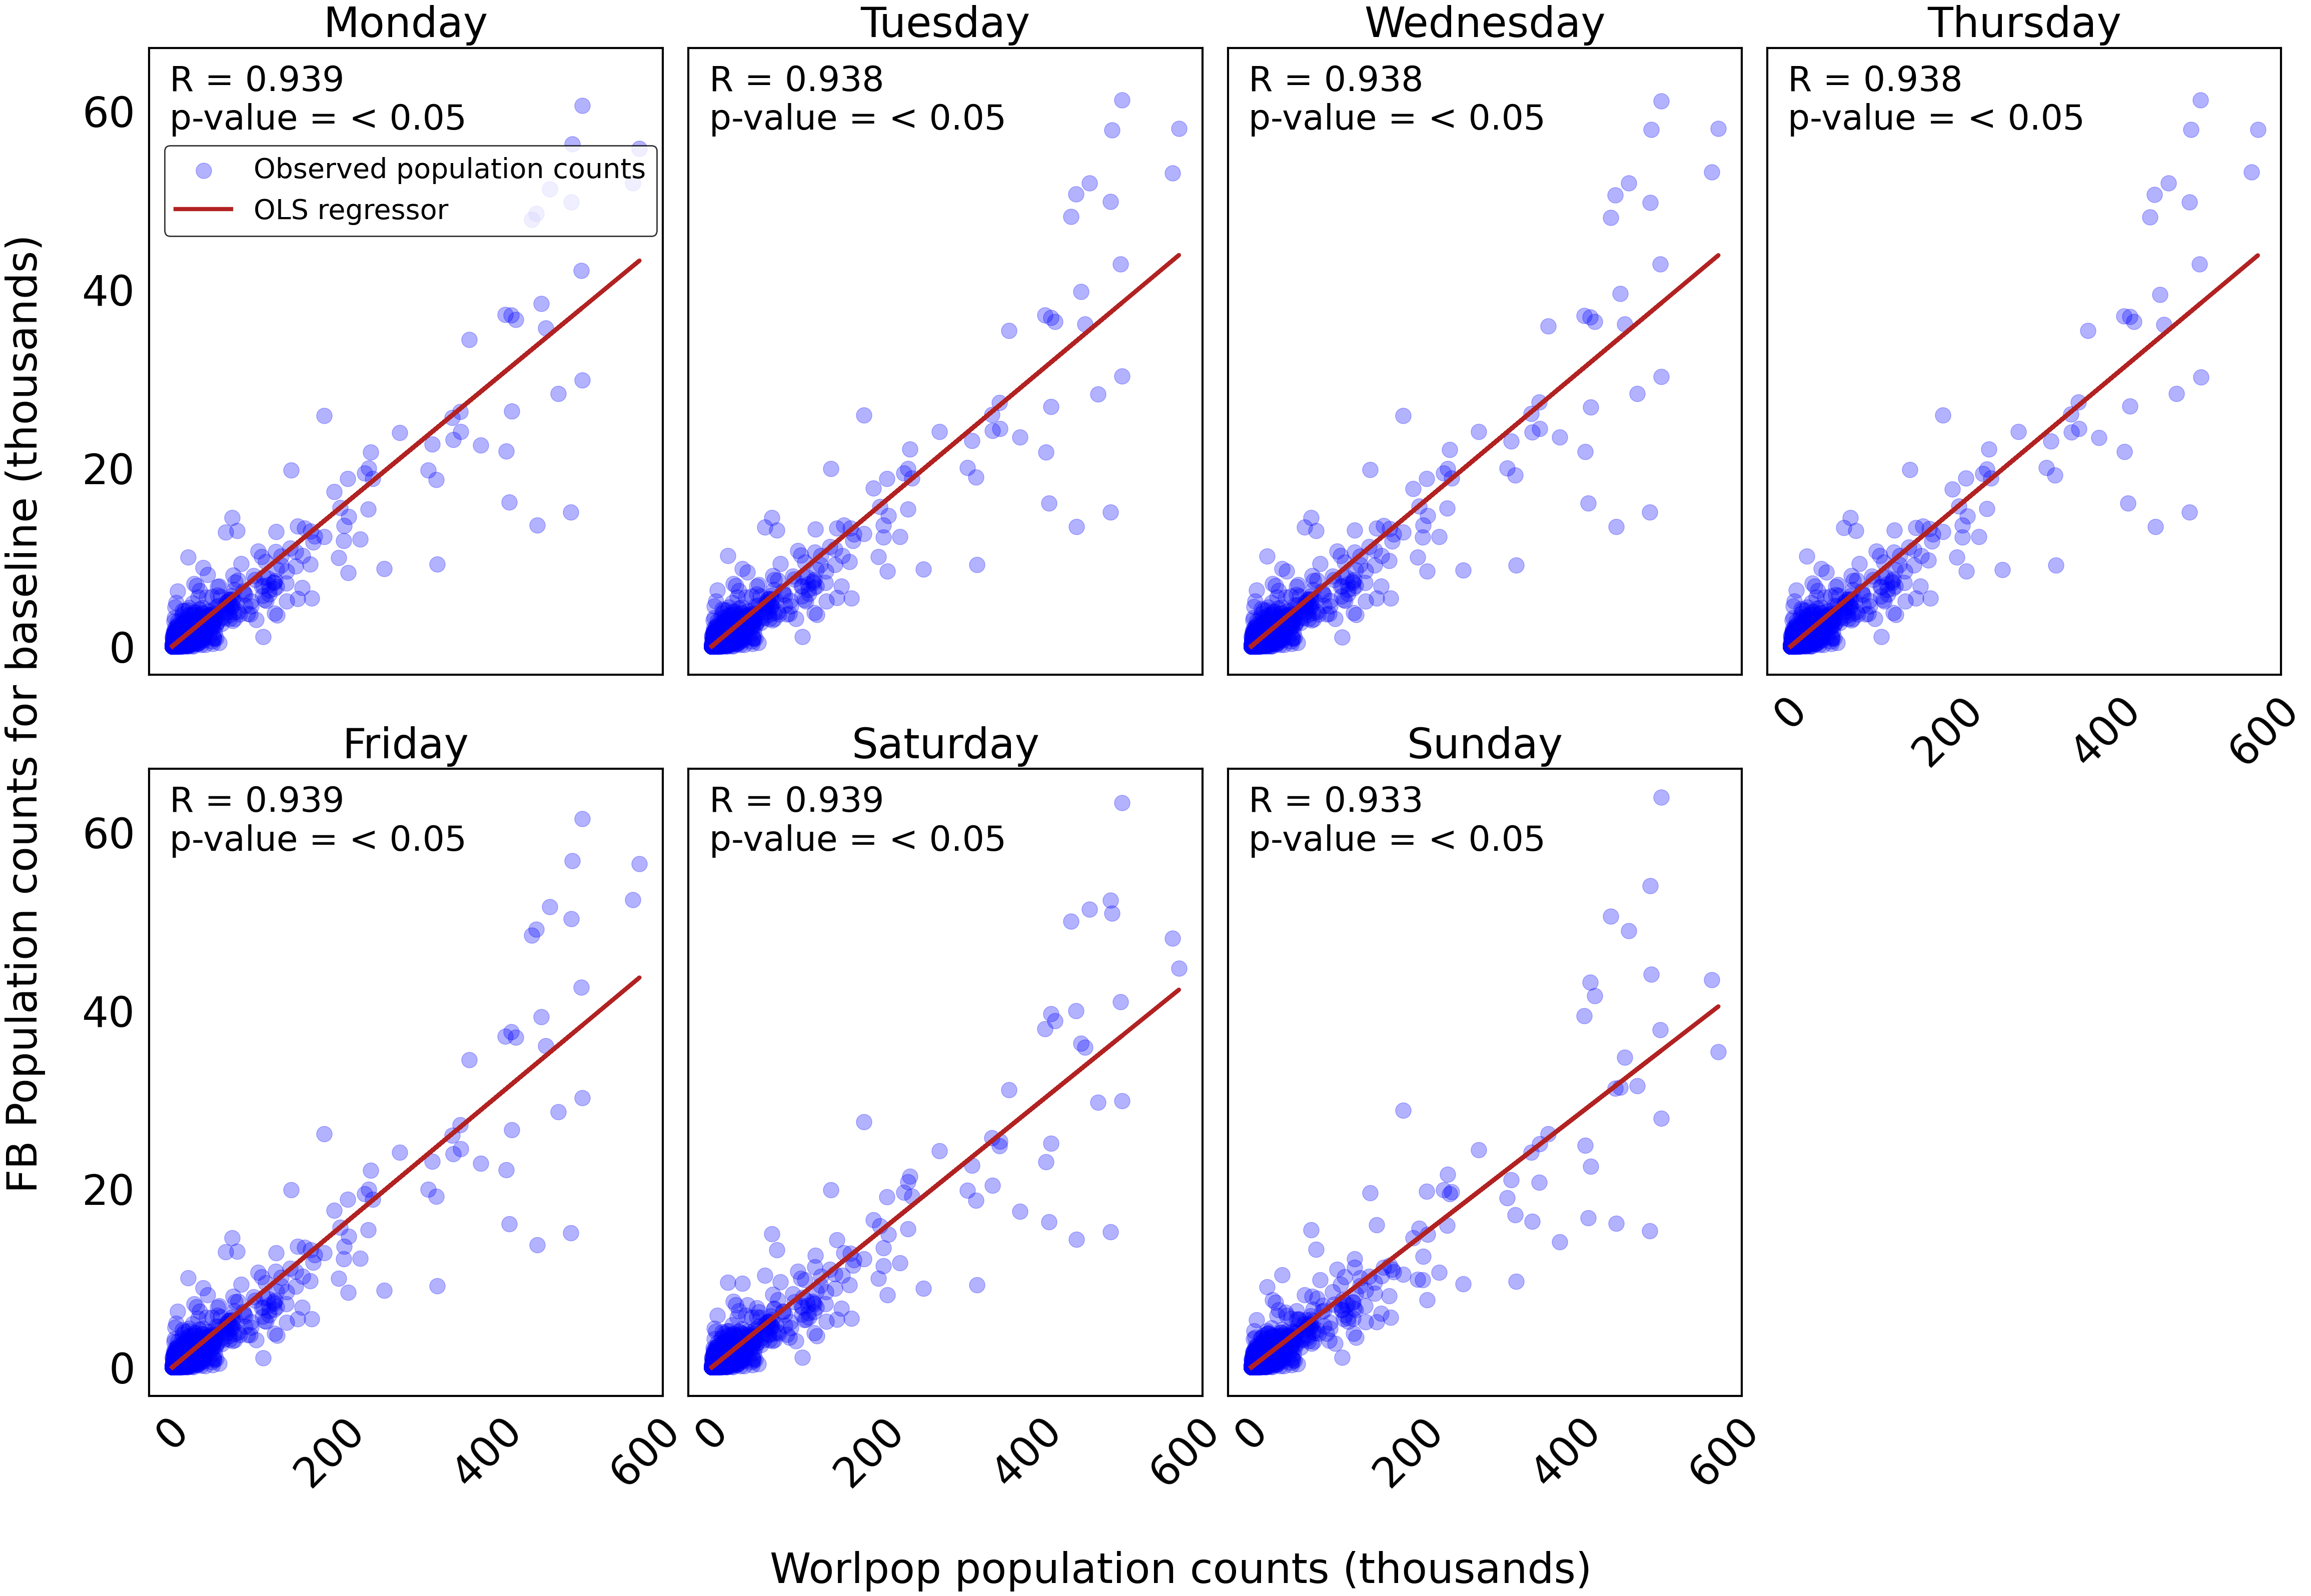
\includegraphics[width=\linewidth]{supplementary/correlation/correlation-wp-fb-pop-baseline-COL.png}
\caption{Correlation between Worldpop population counts and Facebook Population counts during the baseline period in Colombia, for each day of the week.}
\label{correlation-wp-fbpop-COL}
\end{figure}

\newpage

\subsection{Assessing results of spatial interaction model for imputing missing number of movements in baseline}

\begin{figure}[h!]
\centering
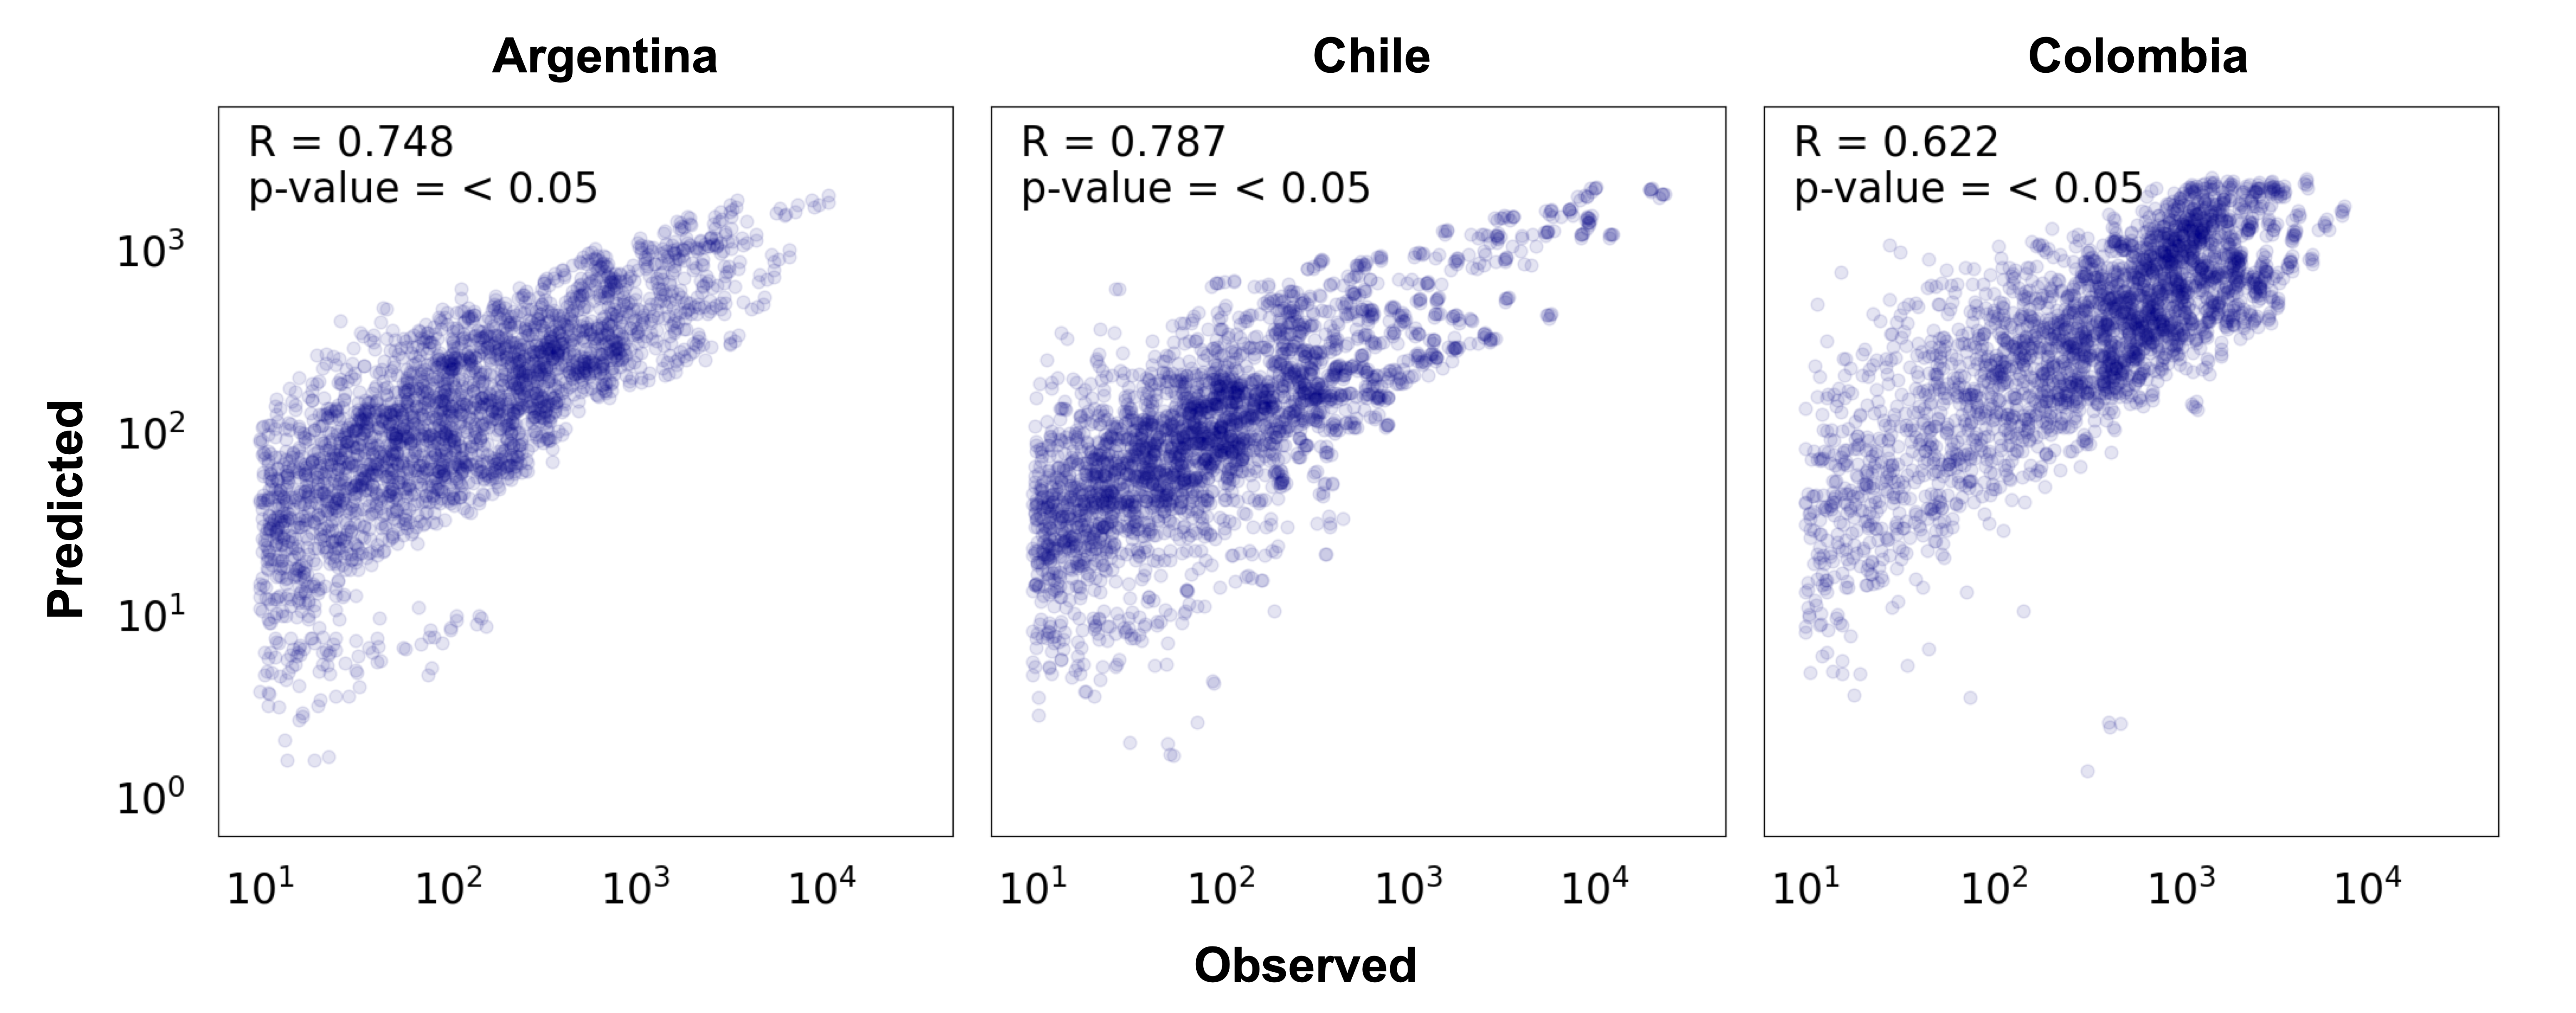
\includegraphics[width=\linewidth]{supplementary/sim/SF-sim-validation.png}
\caption{Relationship between observed and predicted value of number of movements between origin-destination pairs of Bing tiles during the baseline, for all weekdays.}
\end{figure}

\begin{figure}[h!]
\centering
\includegraphics[width=\linewidth]{supplementary/sim/SF-sim-check.png}
\caption{Relationship between Facebook Population at the origin and the destination of each population flow during the baseline period. The Facebook Population is considered after the imputation of the Facebook Population baseline data. The colour of the markers represents the volume of the flows during the baseline period, both observed and predicted through the spatial interaction model. Note that the Bing tiles used to record Facebook Movement data in Colombia are smaller than in Argentina and Chile, hence the lower numbers. }
\end{figure}


\newpage

\section{Classification of tiles according to level of urbanisation and socioeconomic deprivation}

\begin{figure}[h!]
\centering
\includegraphics[width=\linewidth]{supplementary/categories/SF-maps-classes.png}
\caption{Classification of spatial units into categories by population density and by relative deprivation index. Spatial distribution of categories and population share in each category, by country.}
\end{figure}

\begin{figure}[h!]
\centering
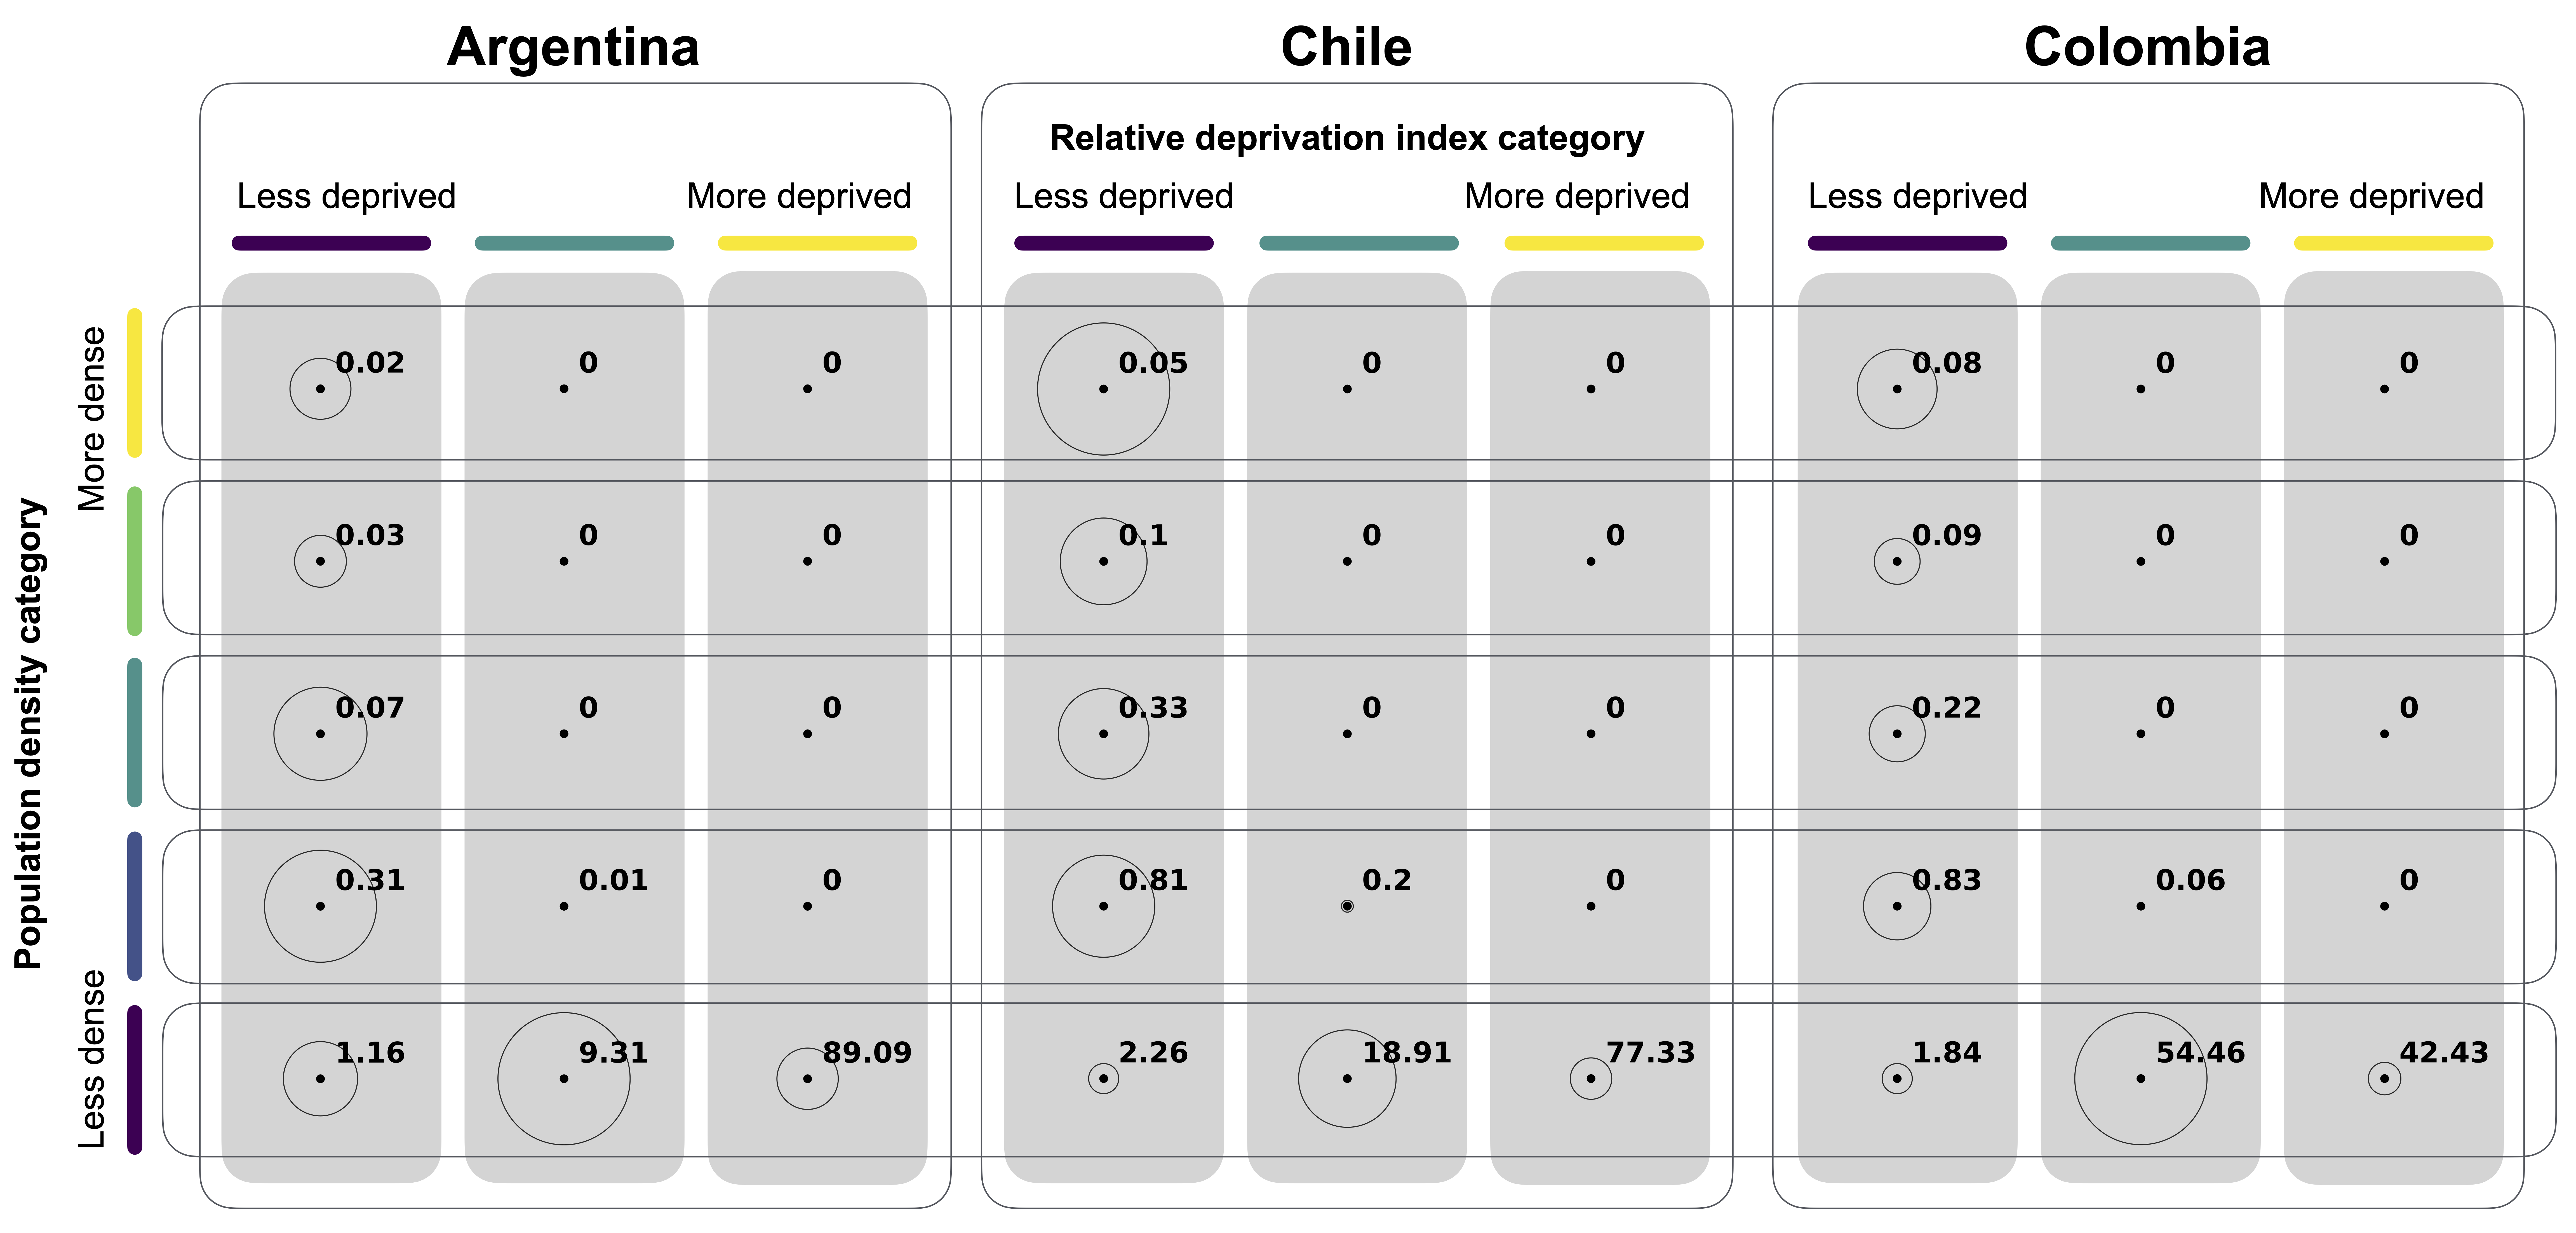
\includegraphics[width=\linewidth]{supplementary/categories/SF-classes-combined.png}
\caption{Joint distribution of spatial units by population density (rows) and relative deprivation index (RDI) categories (columns), with values representing the percentage of spatial units within each country. Circle sizes indicate the total population corresponding to each category pair.}
\end{figure}

\newpage

\section{Trend analysis}

\subsection{Time series to be model with trend analysis}

\begin{figure}[h!]
\centering
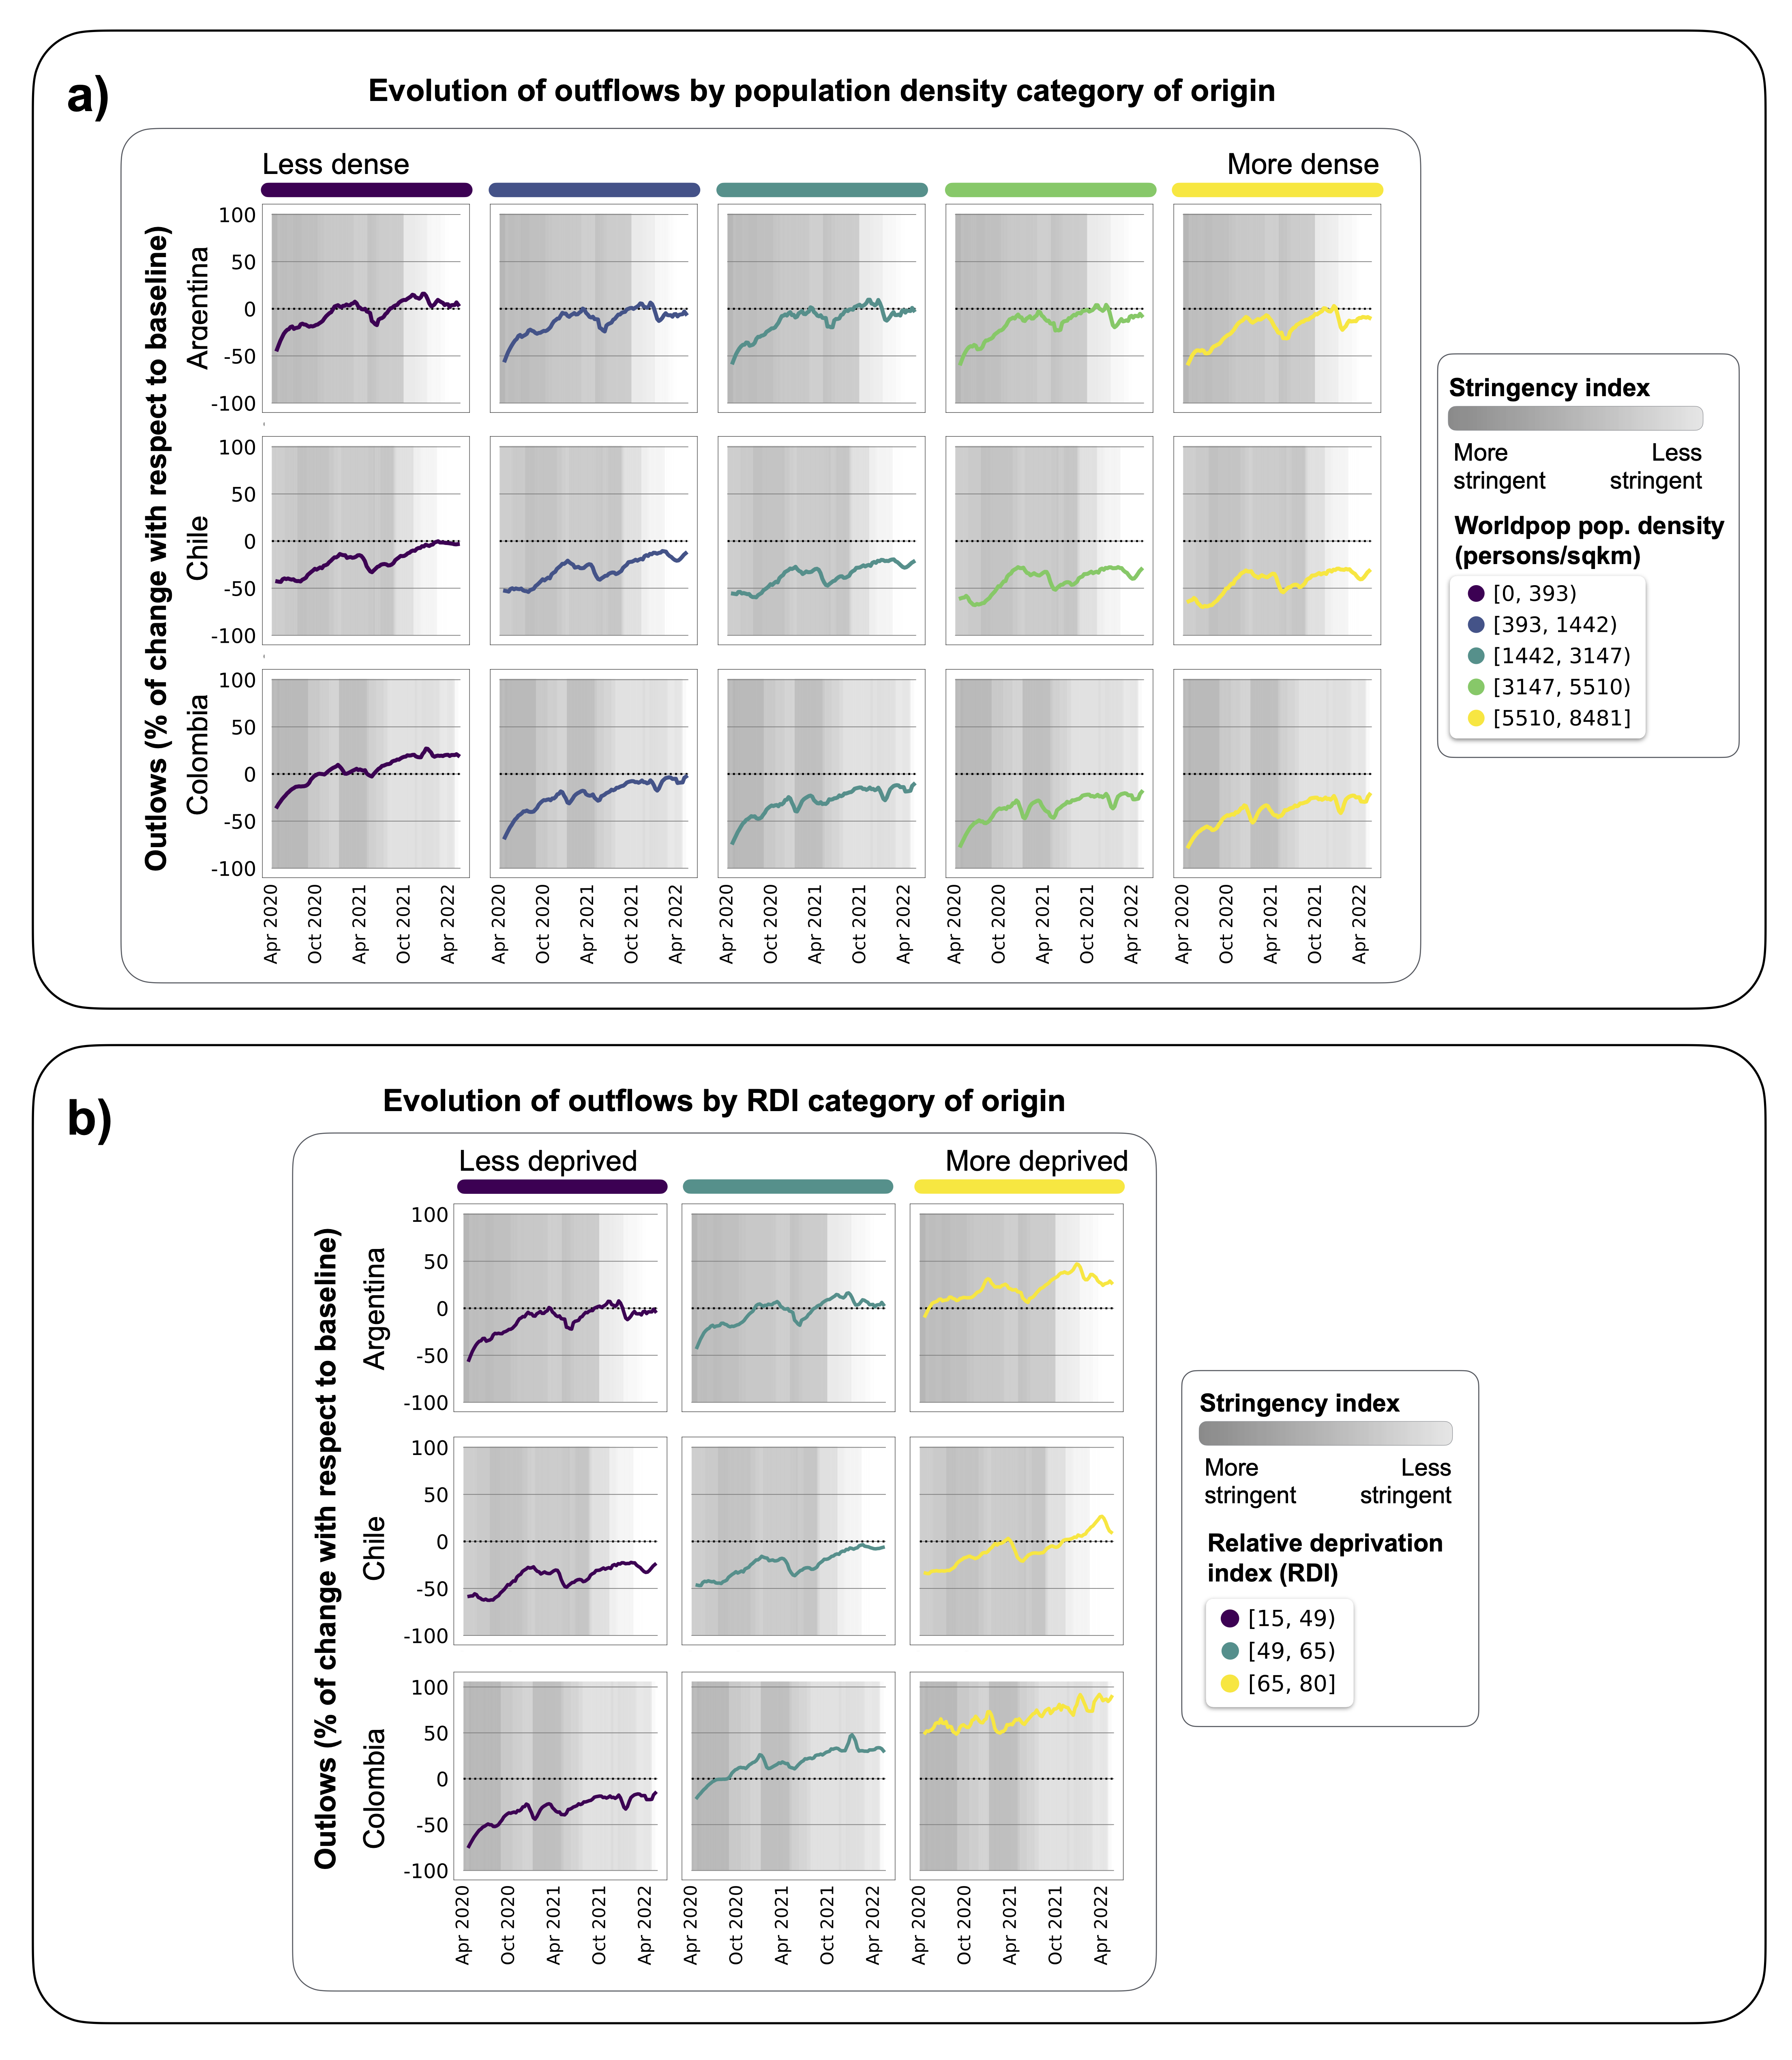
\includegraphics[width=\linewidth]{supplementary/time-series/Fig-recovery-combined-design.png}
\caption{Time evolution of percentage change of outflows relative to pre-pandemic baseline levels, by country and by (a) population density category and (b) relative deprivation category.}
\label{fig-classification}
\end{figure}

\subsection{Mixed effects model specification}

\begin{table}[h!]
\centering
\label{tab:model-specs}
\begin{tabular}{cccccccc}
\toprule
\textbf{Model} & 
\makecell{\textbf{Time} \\ \textbf{(Linear)}} & 
\makecell{\textbf{Time}$^2$} & 
\makecell{\textbf{Origin category} \\ \textbf{(Fixed)}} & 
\makecell{\textbf{Stringency} \\ \textbf{index}} & 
\makecell{\textbf{Random} \\ \textbf{intercept}} & 
\makecell{\textbf{Random slope} \\ \textbf{(Time)}} & 
\makecell{\textbf{Random slope} \\ \textbf{(Time}$^2$\textbf{)}} \\
\midrule
1 & \checkmark & & & (\checkmark) & & & \\
2 & \checkmark & & \checkmark & (\checkmark) & & & \\
3 & \checkmark & & & (\checkmark) & \checkmark & & \\
4 & \checkmark & & & (\checkmark) & & \checkmark & \\
5 & \checkmark & & & (\checkmark) & \checkmark & \checkmark & \\
6 & \checkmark & \checkmark & & (\checkmark) & \checkmark & \checkmark & \\
7 & \checkmark & \checkmark & & (\checkmark) & \checkmark & \checkmark & \checkmark \\
\end{tabular}
\caption{Summary of mixed-effects model specifications. There is a total of 14. Each row in the table represents a pair of models: one that includes the stringency index as a covariate and one that excludes it. This is denoted by a bracketed check mark [(\checkmark)]. All other check marks [\checkmark] indicate terms that are included in both models of the pair. Random effects are considered according to the population density or the Relative Deprivation Index (RDI) of the origin location of outflows.}
\end{table}

\newpage

\subsection{Relative change in outflows}

\begin{table}[h!]
\centering
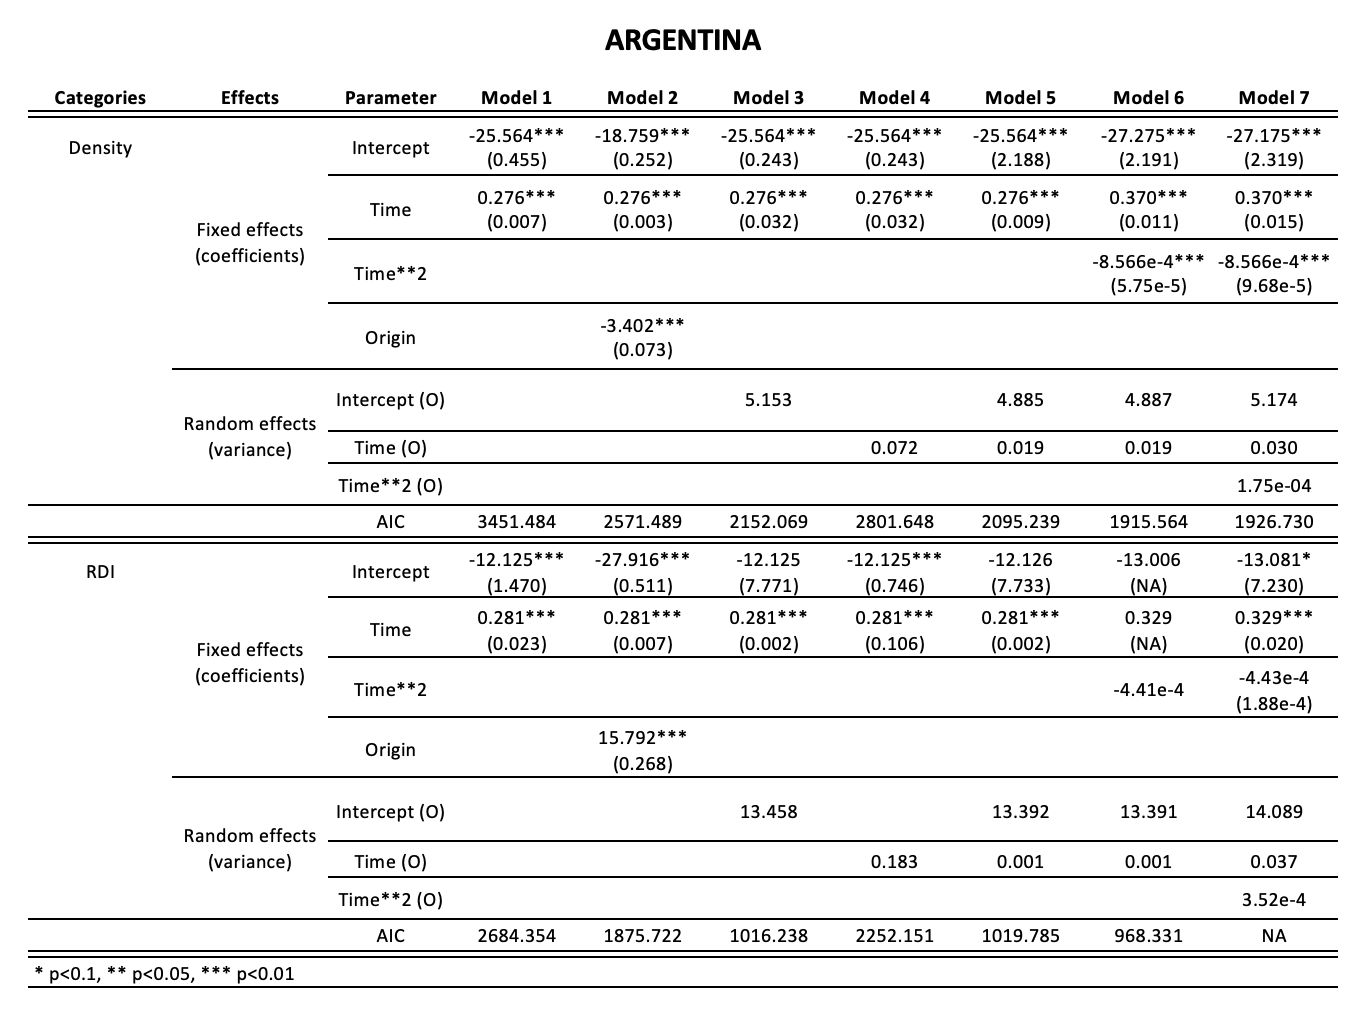
\includegraphics[width=\linewidth]{supplementary/models-tables/models-table-ARG-quadratic.png}
\caption{Results of mixed-effects models for trend analysis of relative change in outflows in Argentina. Random effects according to the population density or the Relative Deprivation Index (RDI) of the origin location of outflows.}
\end{table}

\newpage

\begin{table}[h!]
\centering
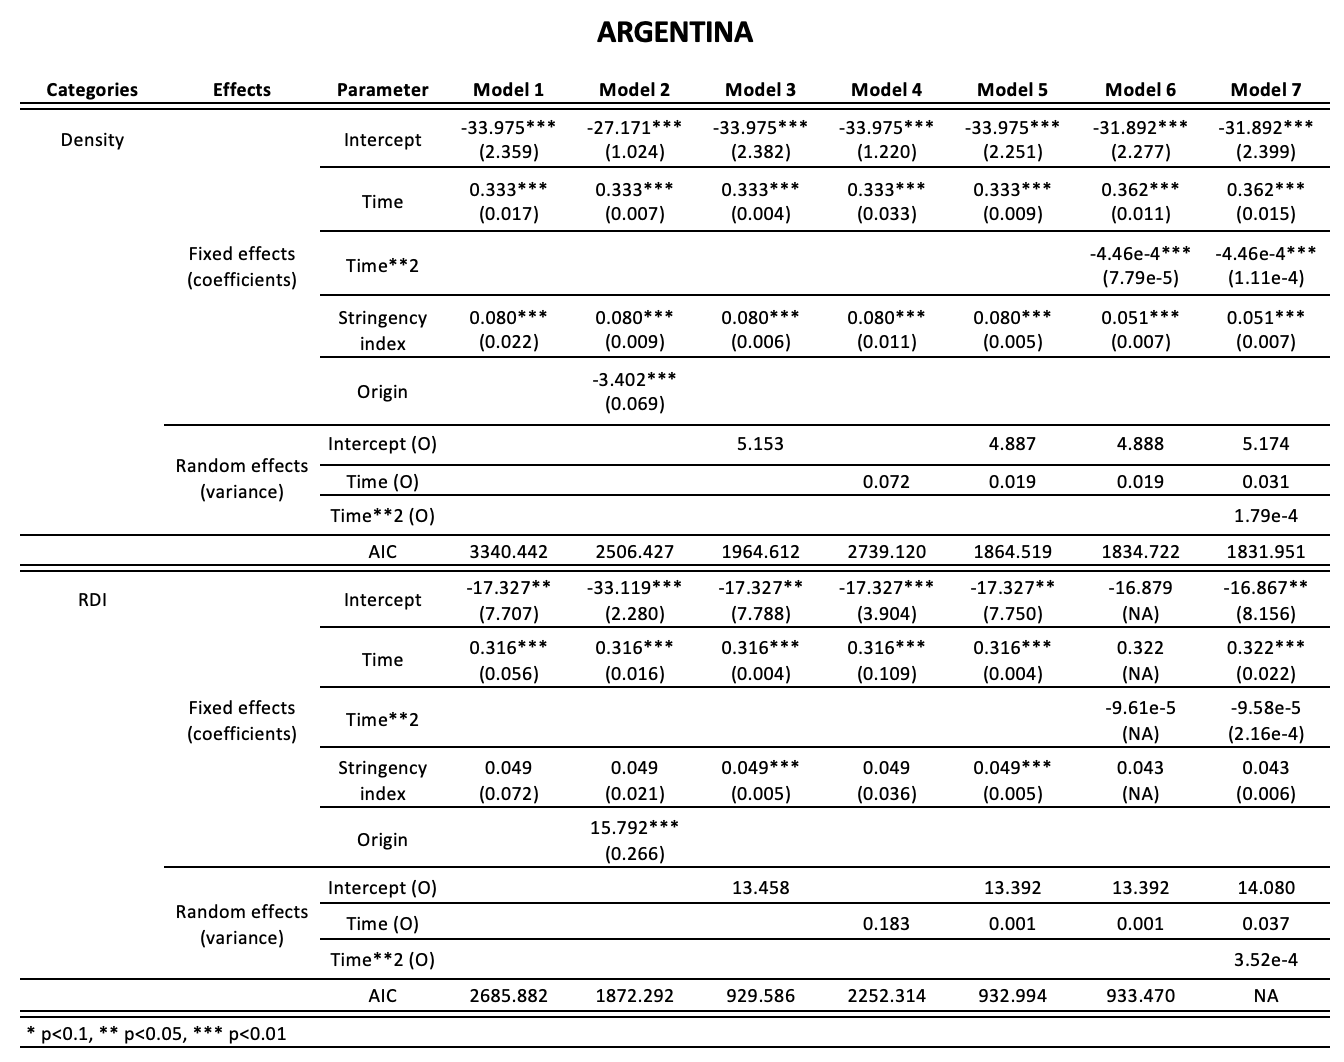
\includegraphics[width=\linewidth]{supplementary/models-tables/models-table-ARG-quadratic-stringency.png}
\caption{Results of mixed-effects models for trend analysis of relative change in outflows in Argentina including stringency index as a predictor variable. Random effects according to the population density or the Relative Deprivation Index (RDI) of the origin location of outflows.}
\label{tab-modelsARG-stringency}
\end{table}

\newpage

\begin{table}[h!]
\centering
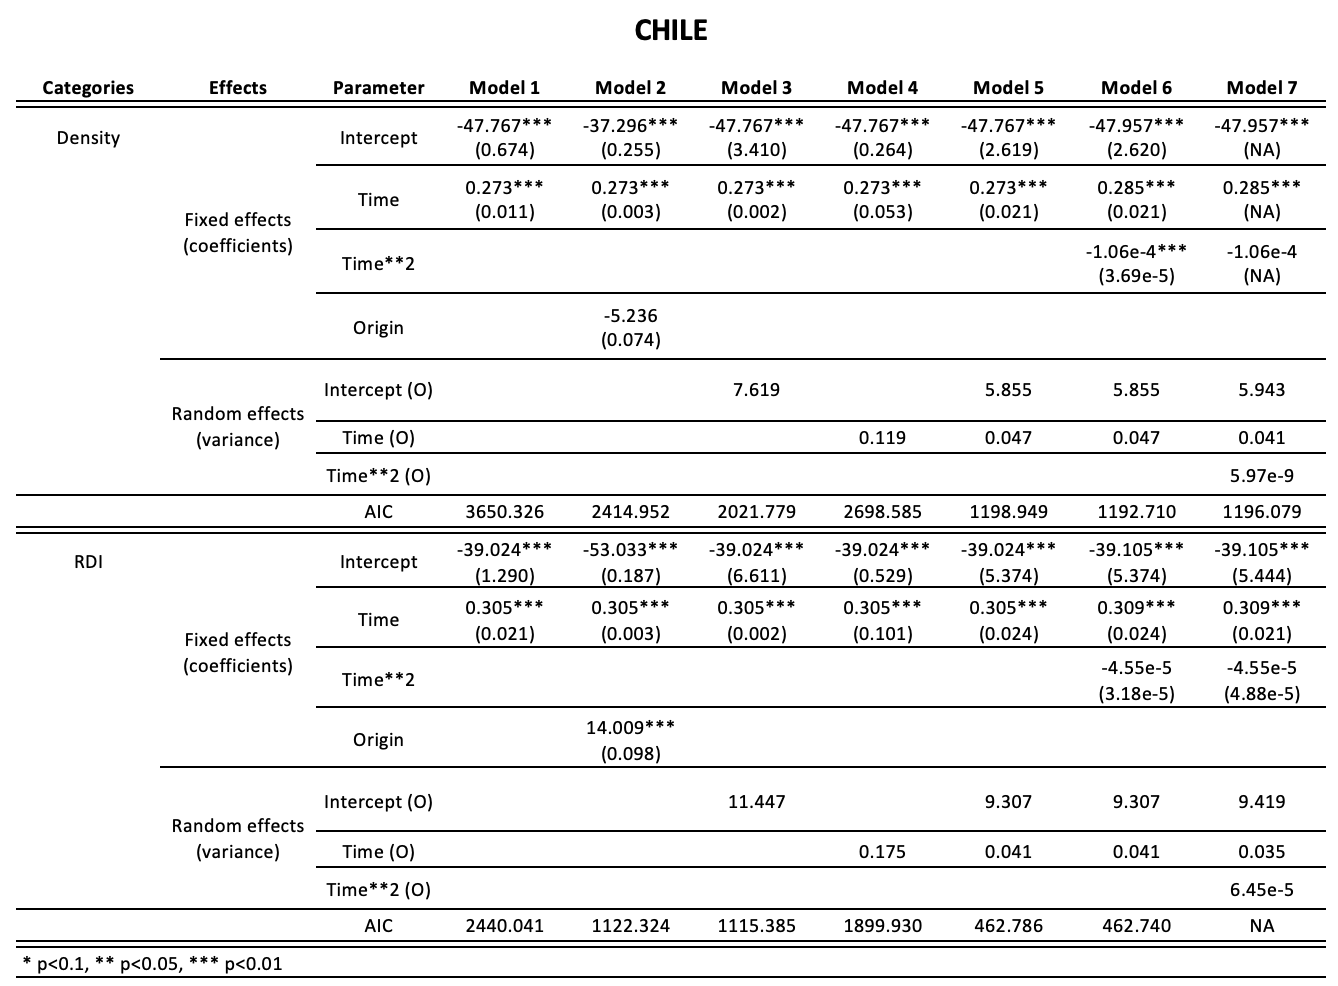
\includegraphics[width=\linewidth]{supplementary/models-tables/models-table-CHL-quadratic.png}
\caption{Results of mixed-effects models for trend analysis of relative change in outflows in Chile. Random effects according to the population density or the Relative Deprivation Index (RDI) of the origin location of outflows.}
\label{tab-modelsCHL}
\end{table}

\newpage

\begin{table}[h!]
\centering
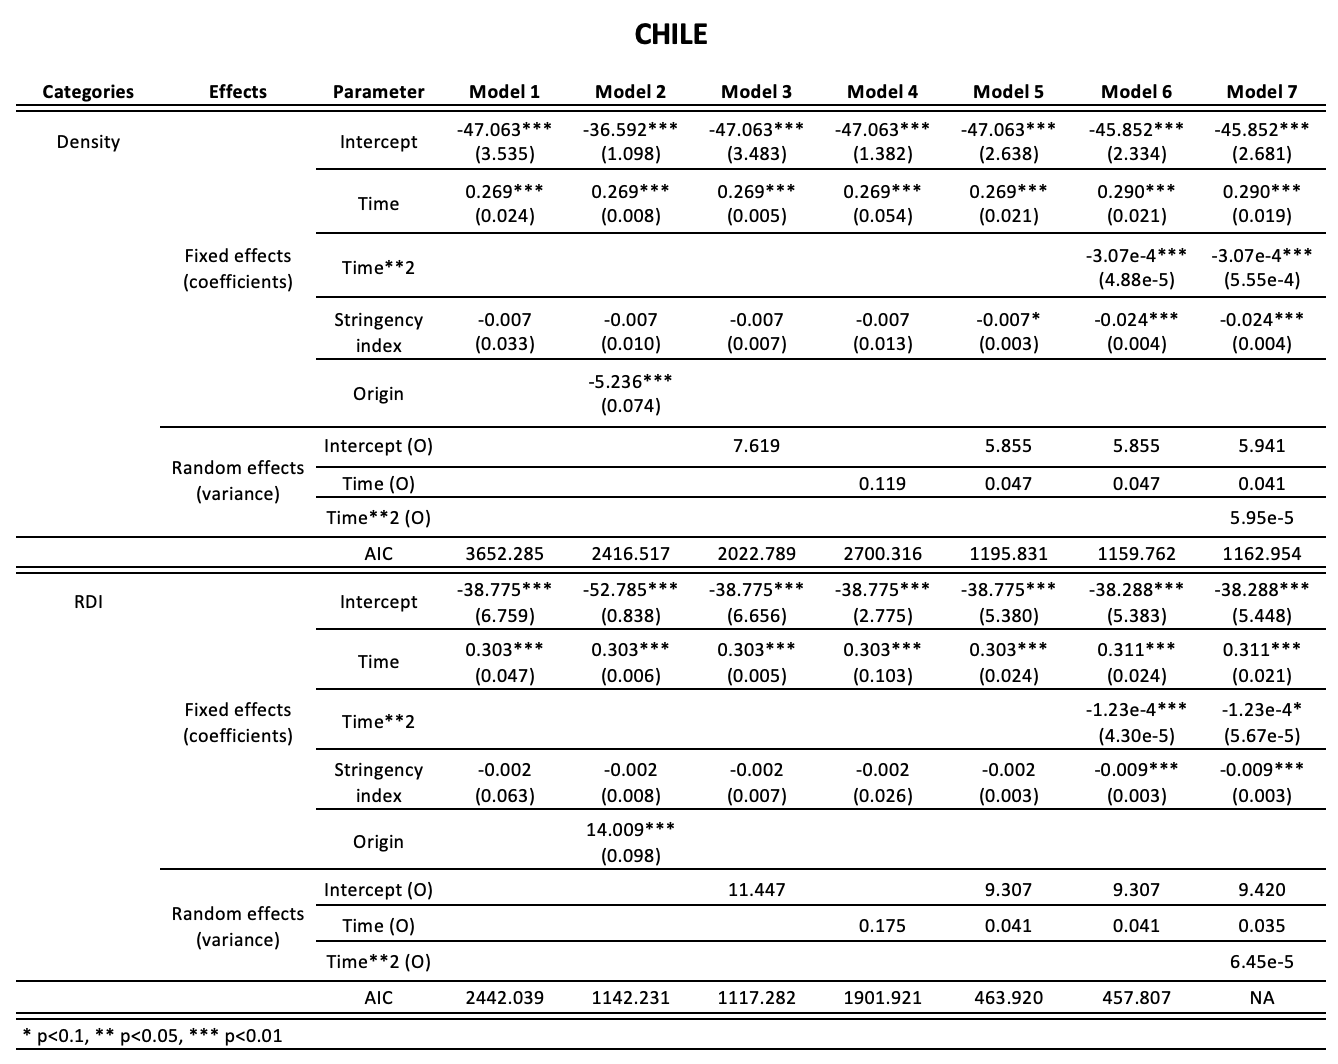
\includegraphics[width=\linewidth]{supplementary/models-tables/models-table-CHL-quadratic-stringency.png}
\caption{Results of mixed-effects models for trend analysis of relative change in outflows in Chile including stringency index as a predictor variable. Random effects according to the population density or the Relative Deprivation Index (RDI) of the origin location of outflows.}
\label{tab-modelsCHL-stringency}
\end{table}

\newpage

\begin{table}[h!]
\centering
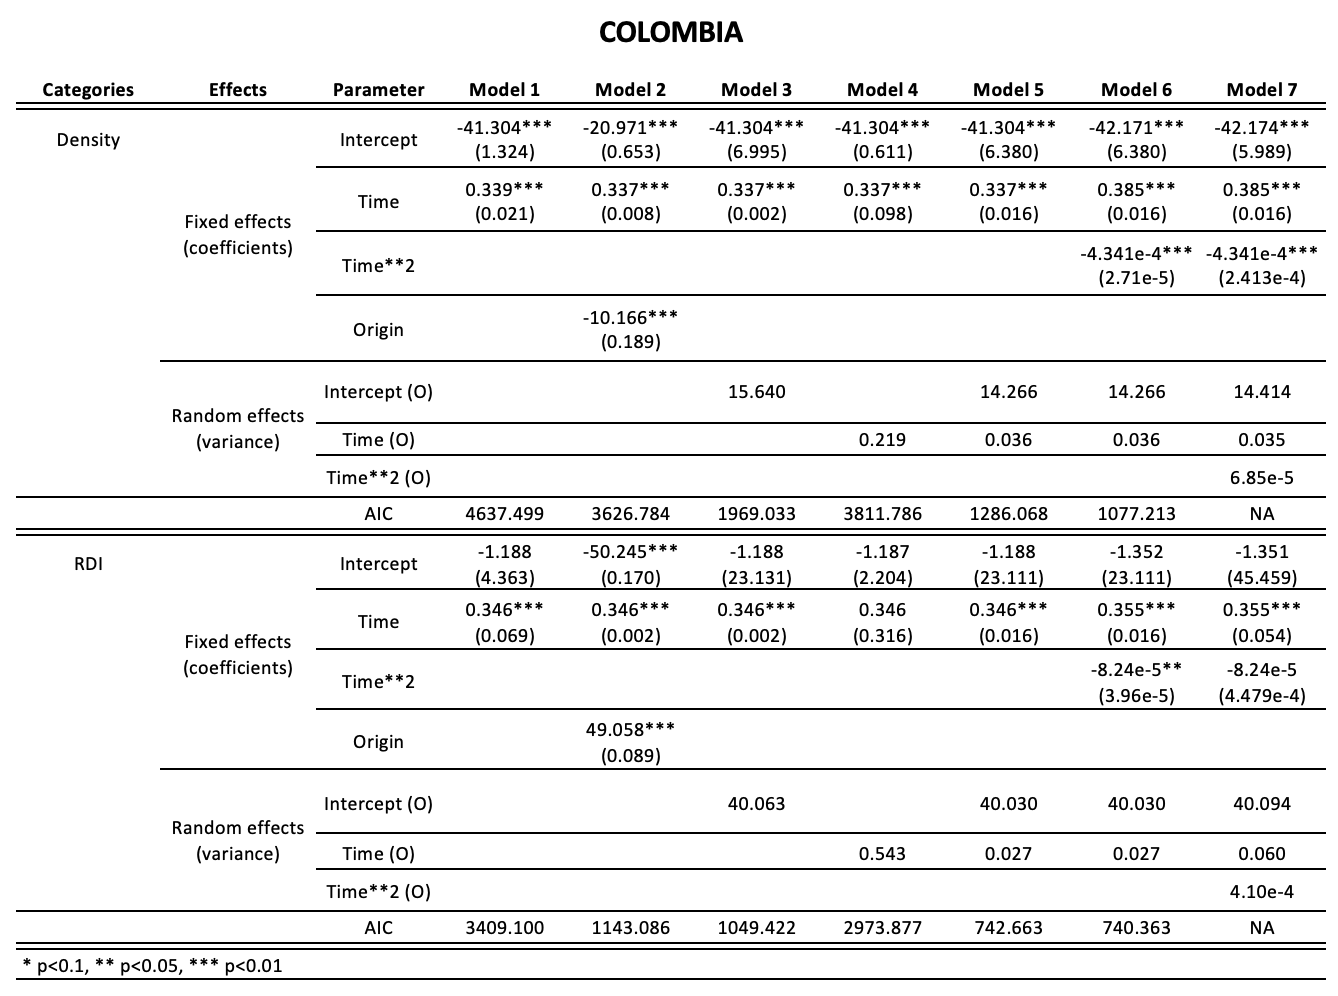
\includegraphics[width=\linewidth]{supplementary/models-tables/models-table-COL-quadratic.png}
\caption{Results of mixed-effects models for trend analysis of relative change in outflows in Colombia. Random effects according to the population density or the Relative Deprivation Index (RDI) of the origin location of outflows.}
\label{tab-modelsCOL}
\end{table}

\newpage

\begin{table}[h!]
\centering
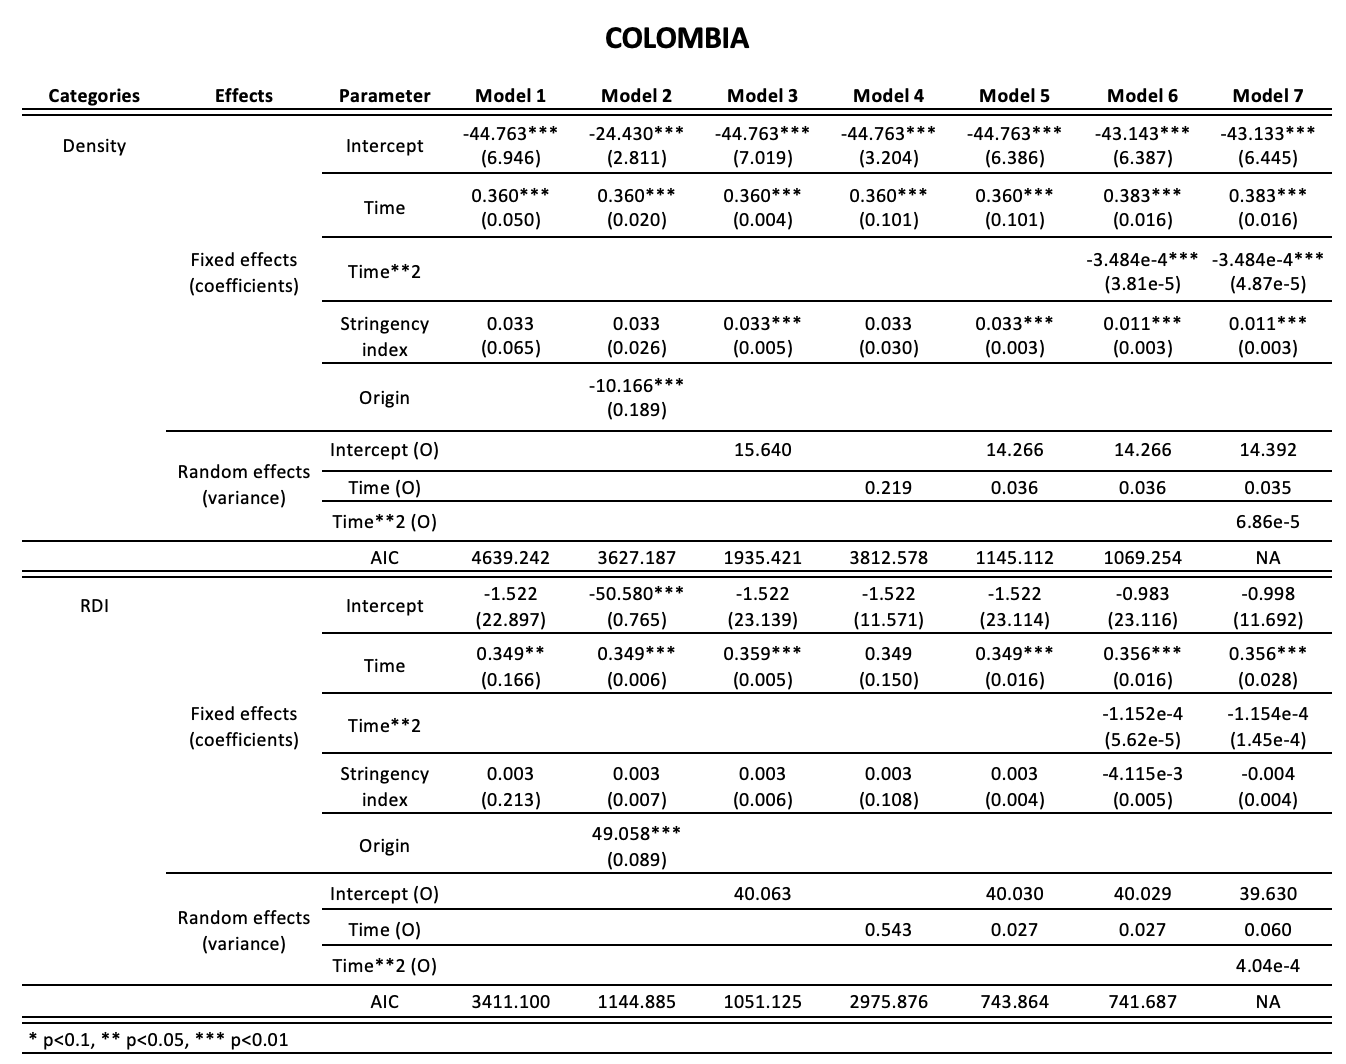
\includegraphics[width=\linewidth]{supplementary/models-tables/models-table-COL-quadratic-stringency.png}
\caption{Results of mixed-effects models for trend analysis of relative change in outflows in Colombia including stringency index as a predictor variable. Random effects according to the population density or the Relative Deprivation Index (RDI) of the origin location of outflows.}
\label{tab-modelsCOL-stringency}
\end{table}

\newpage

\subsection{Relative change in netflows involving capital}

\begin{table}[h!]
\centering
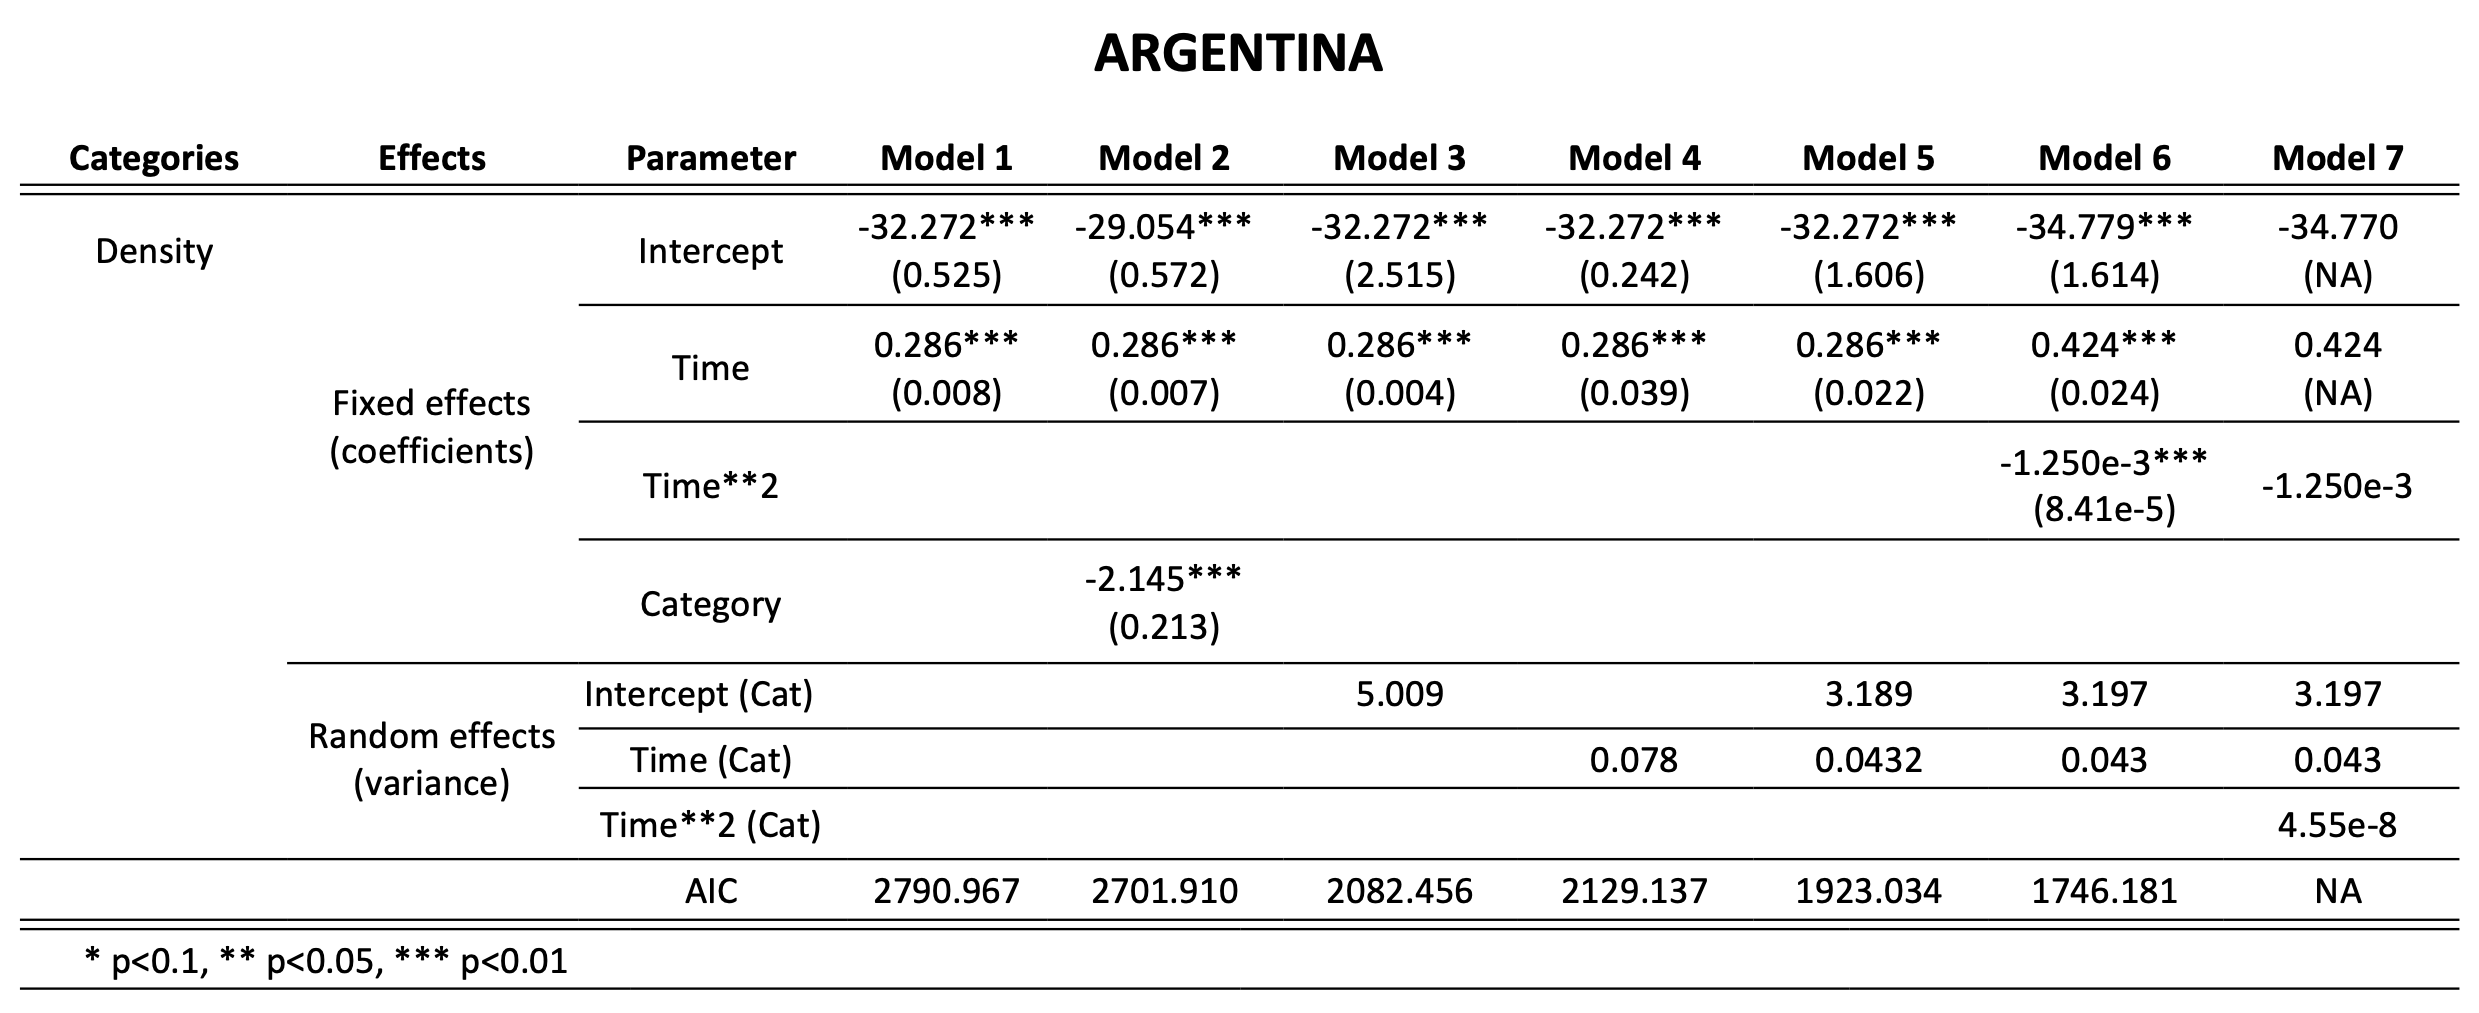
\includegraphics[width=\linewidth]{supplementary/models-tables/models-table-ARG-quadratic-capital.png}
\caption{Results of mixed-effects models for trend analysis of relative change in netflows involving urban region surrounding capital in Argentina. Netflows are defined as inflows to an urban core minus outflows from the urban core. Random effects according to the population density or the Relative Deprivation Index (RDI) of the origin location of outflows.}
\label{tab-modelsARG-capital}
\end{table}


\begin{table}[h!]
\centering
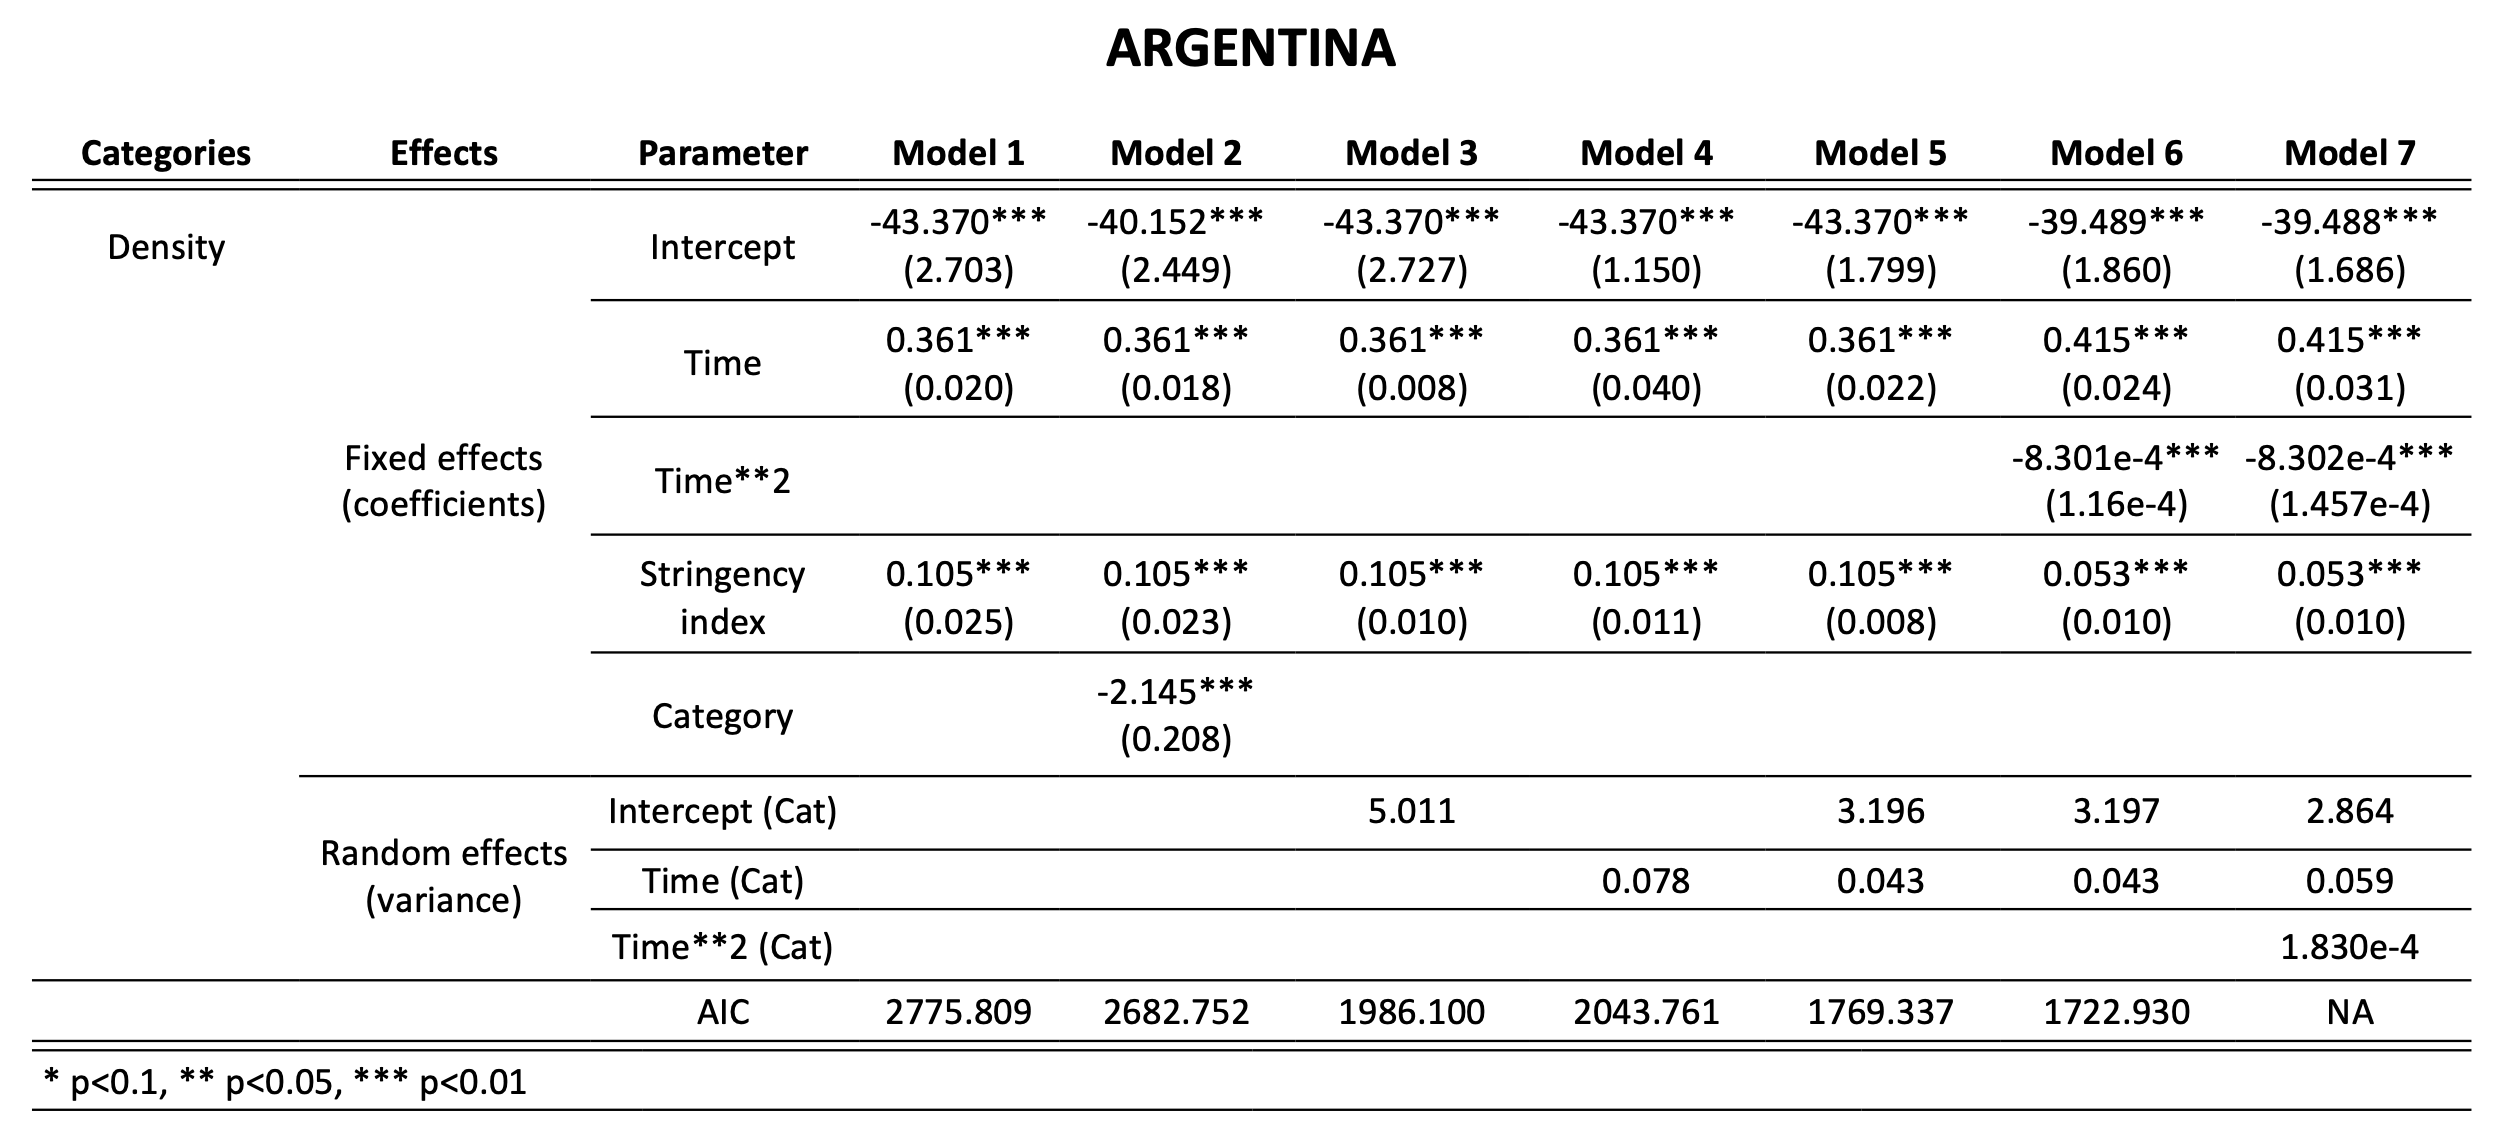
\includegraphics[width=\linewidth]{supplementary/models-tables/models-table-ARG-quadratic-capital-stringency.png}
\caption{Results of mixed-effects models for trend analysis of relative change in netflows involving urban region surrounding capital in Argentina including stringency index as a predictor variable. Netflows are defined as inflows to an urban core minus outflows from the urban core. Random effects according to the population density or the Relative Deprivation Index (RDI) of the origin location of outflows.}
\label{tab-modelsARG-capital-stringency}
\end{table}

\newpage

\begin{table}[h!]
\centering
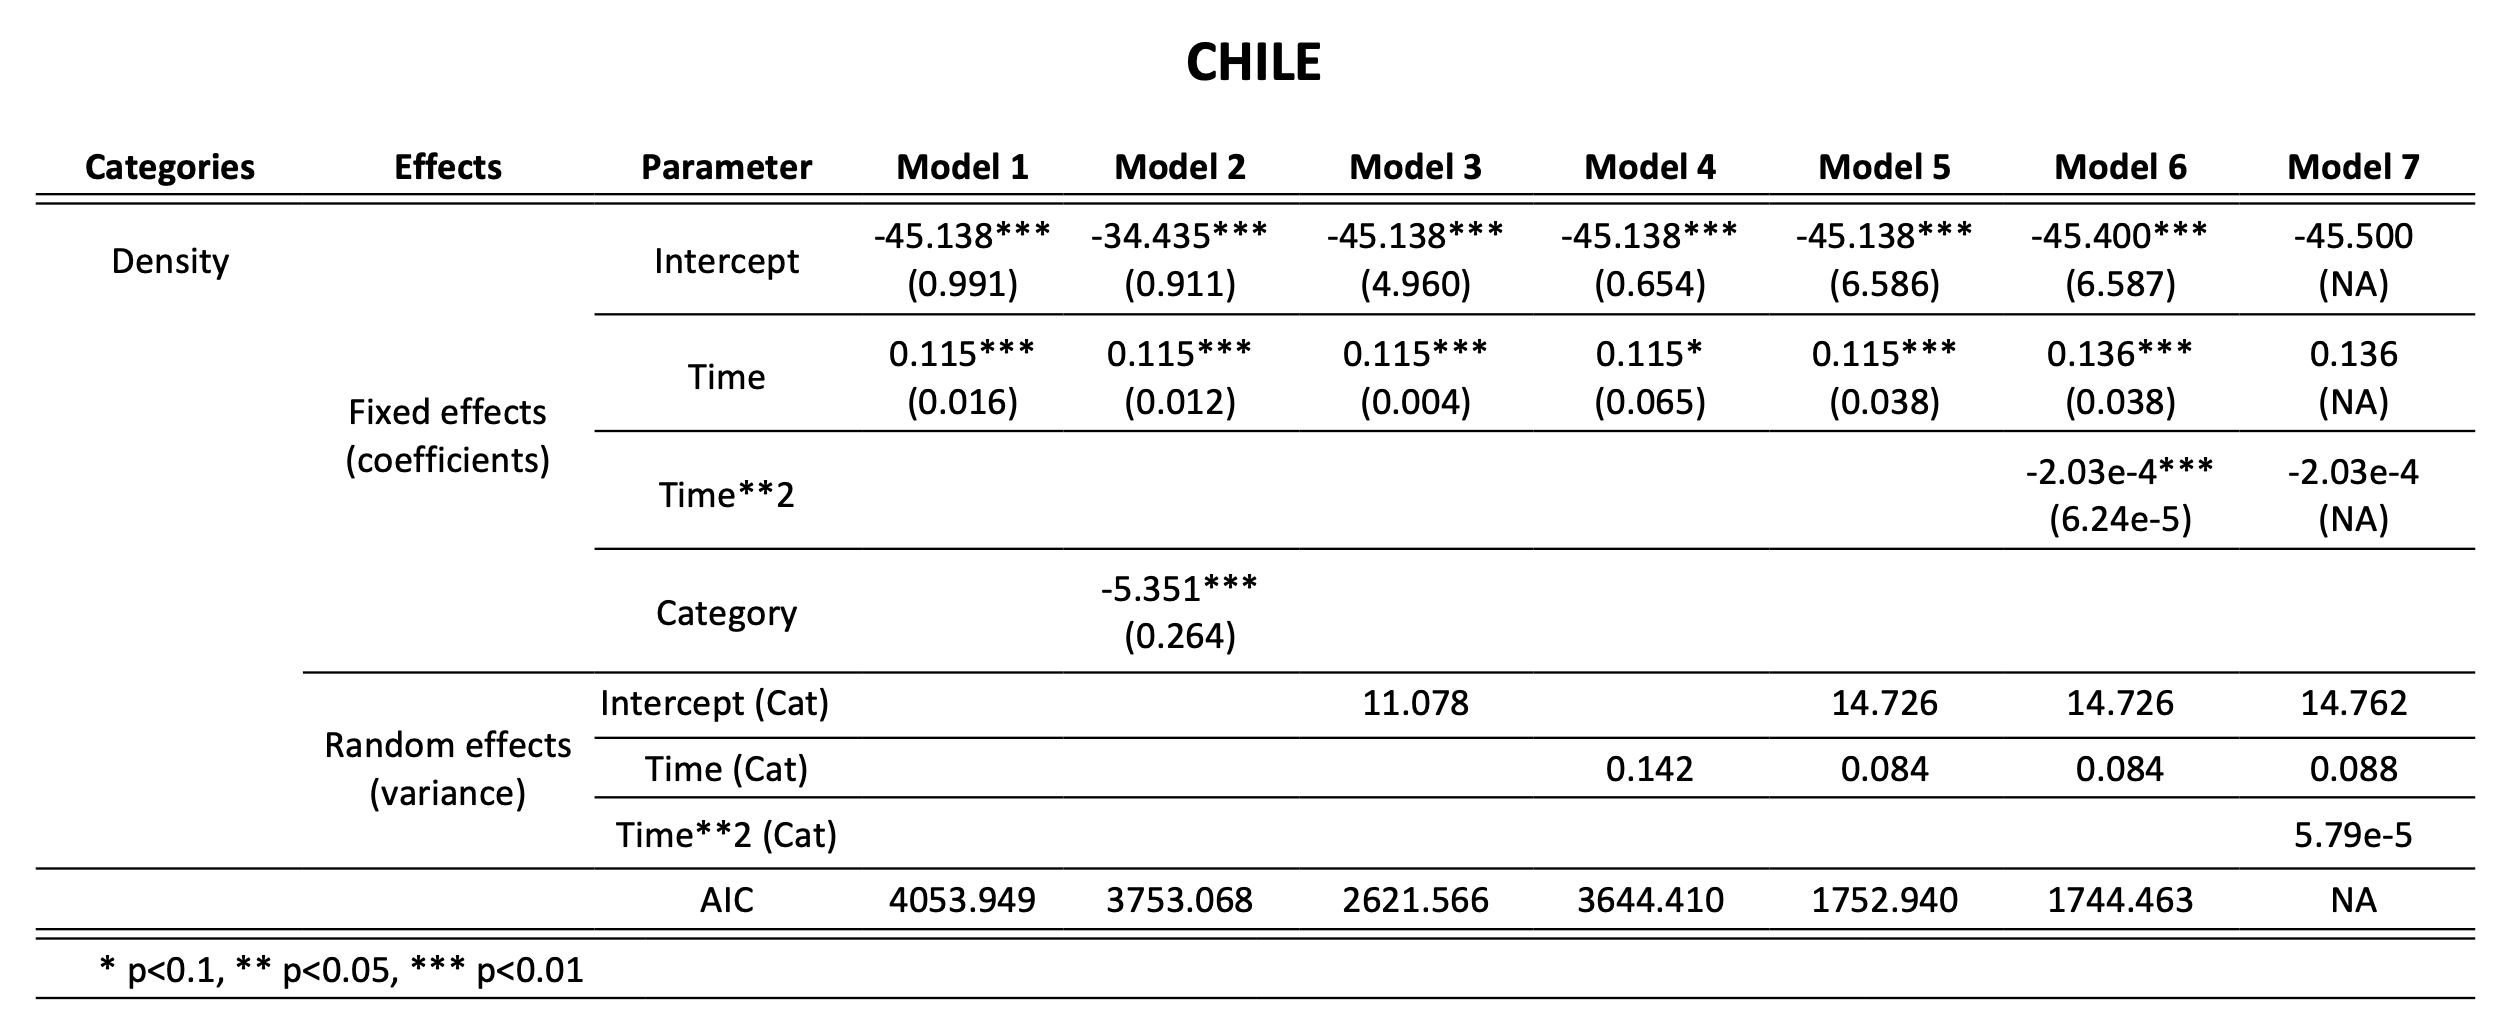
\includegraphics[width=\linewidth]{supplementary/models-tables/models-table-CHL-quadratic-capital.png}
\caption{Results of mixed-effects models for trend analysis of relative change in netflows involving urban region surrounding capital in Chile. Netflows are defined as inflows to an urban core minus outflows from the urban core. Random effects according to the population density or the Relative Deprivation Index (RDI) of the origin location of outflows.}
\label{tab-modelsCHL-capital}
\end{table}


\begin{table}[h!]
\centering
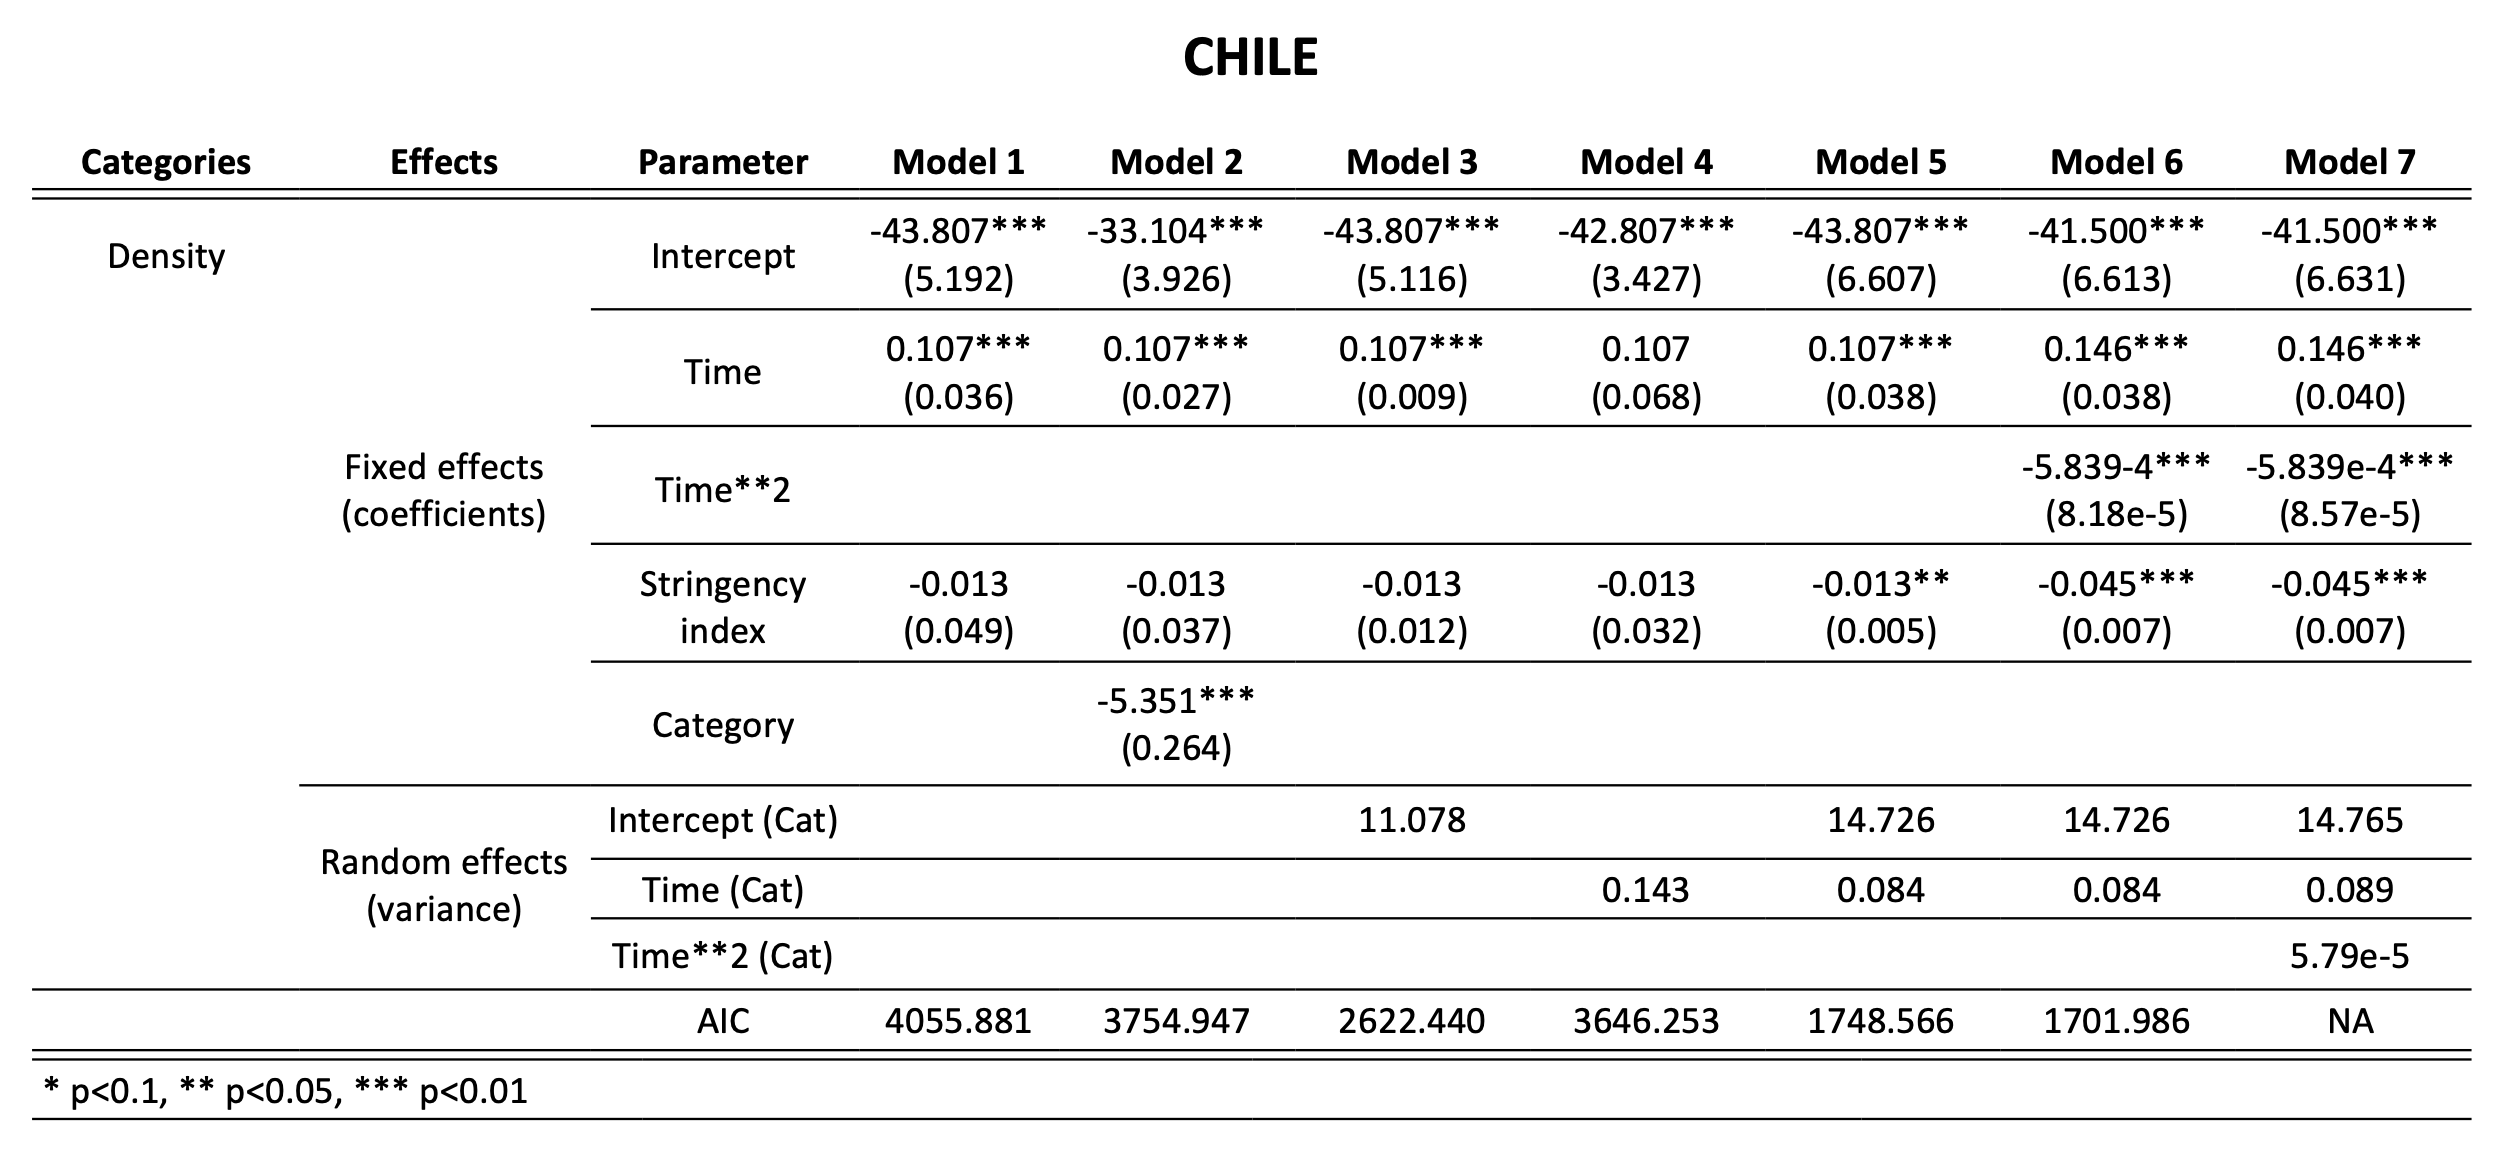
\includegraphics[width=\linewidth]{supplementary/models-tables/models-table-CHL-quadratic-capital-stringency.png}
\caption{Results of mixed-effects models for trend analysis of relative change in netflows involving urban region surrounding capital in Chile including stringency index as a predictor variable. Netflows are defined as inflows to an urban core minus outflows from the urban core. Random effects according to the population density or the Relative Deprivation Index (RDI) of the origin location of outflows.}
\label{tab-modelsCHL-capital-stringency}
\end{table}

\newpage

\begin{table}[h!]
\centering
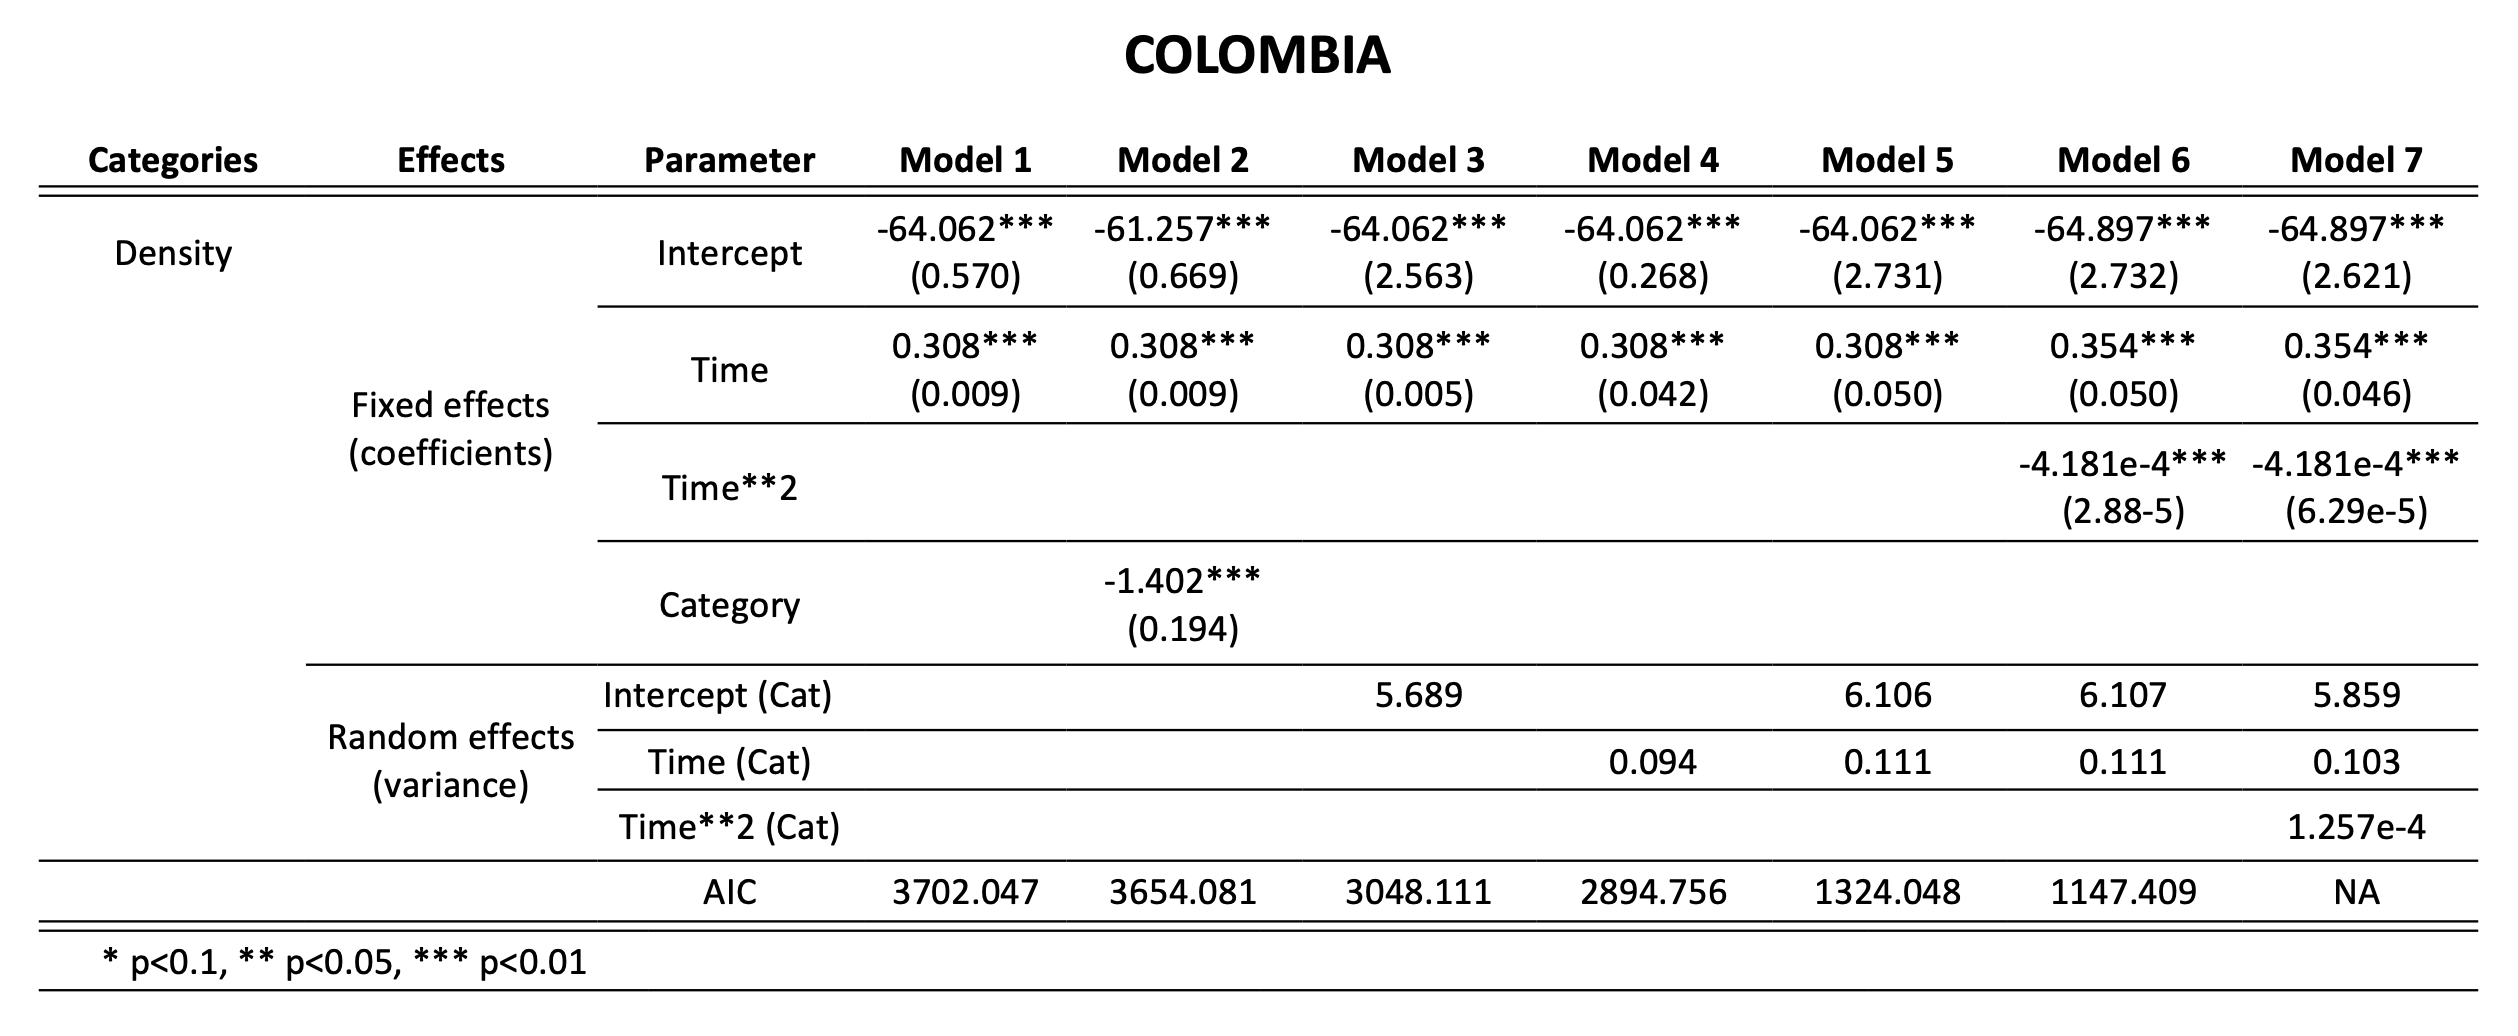
\includegraphics[width=\linewidth]{supplementary/models-tables/models-table-COL-quadratic-capital.png}
\caption{Results of mixed-effects models for trend analysis of relative change in netflows involving urban region surrounding capital in Colombia. Netflows are defined as inflows to an urban core minus outflows from the urban core. Random effects according to the population density or the Relative Deprivation Index (RDI) of the origin location of outflows.}
\label{tab-modelsCOL-capital}
\end{table}

\begin{table}[h!]
\centering
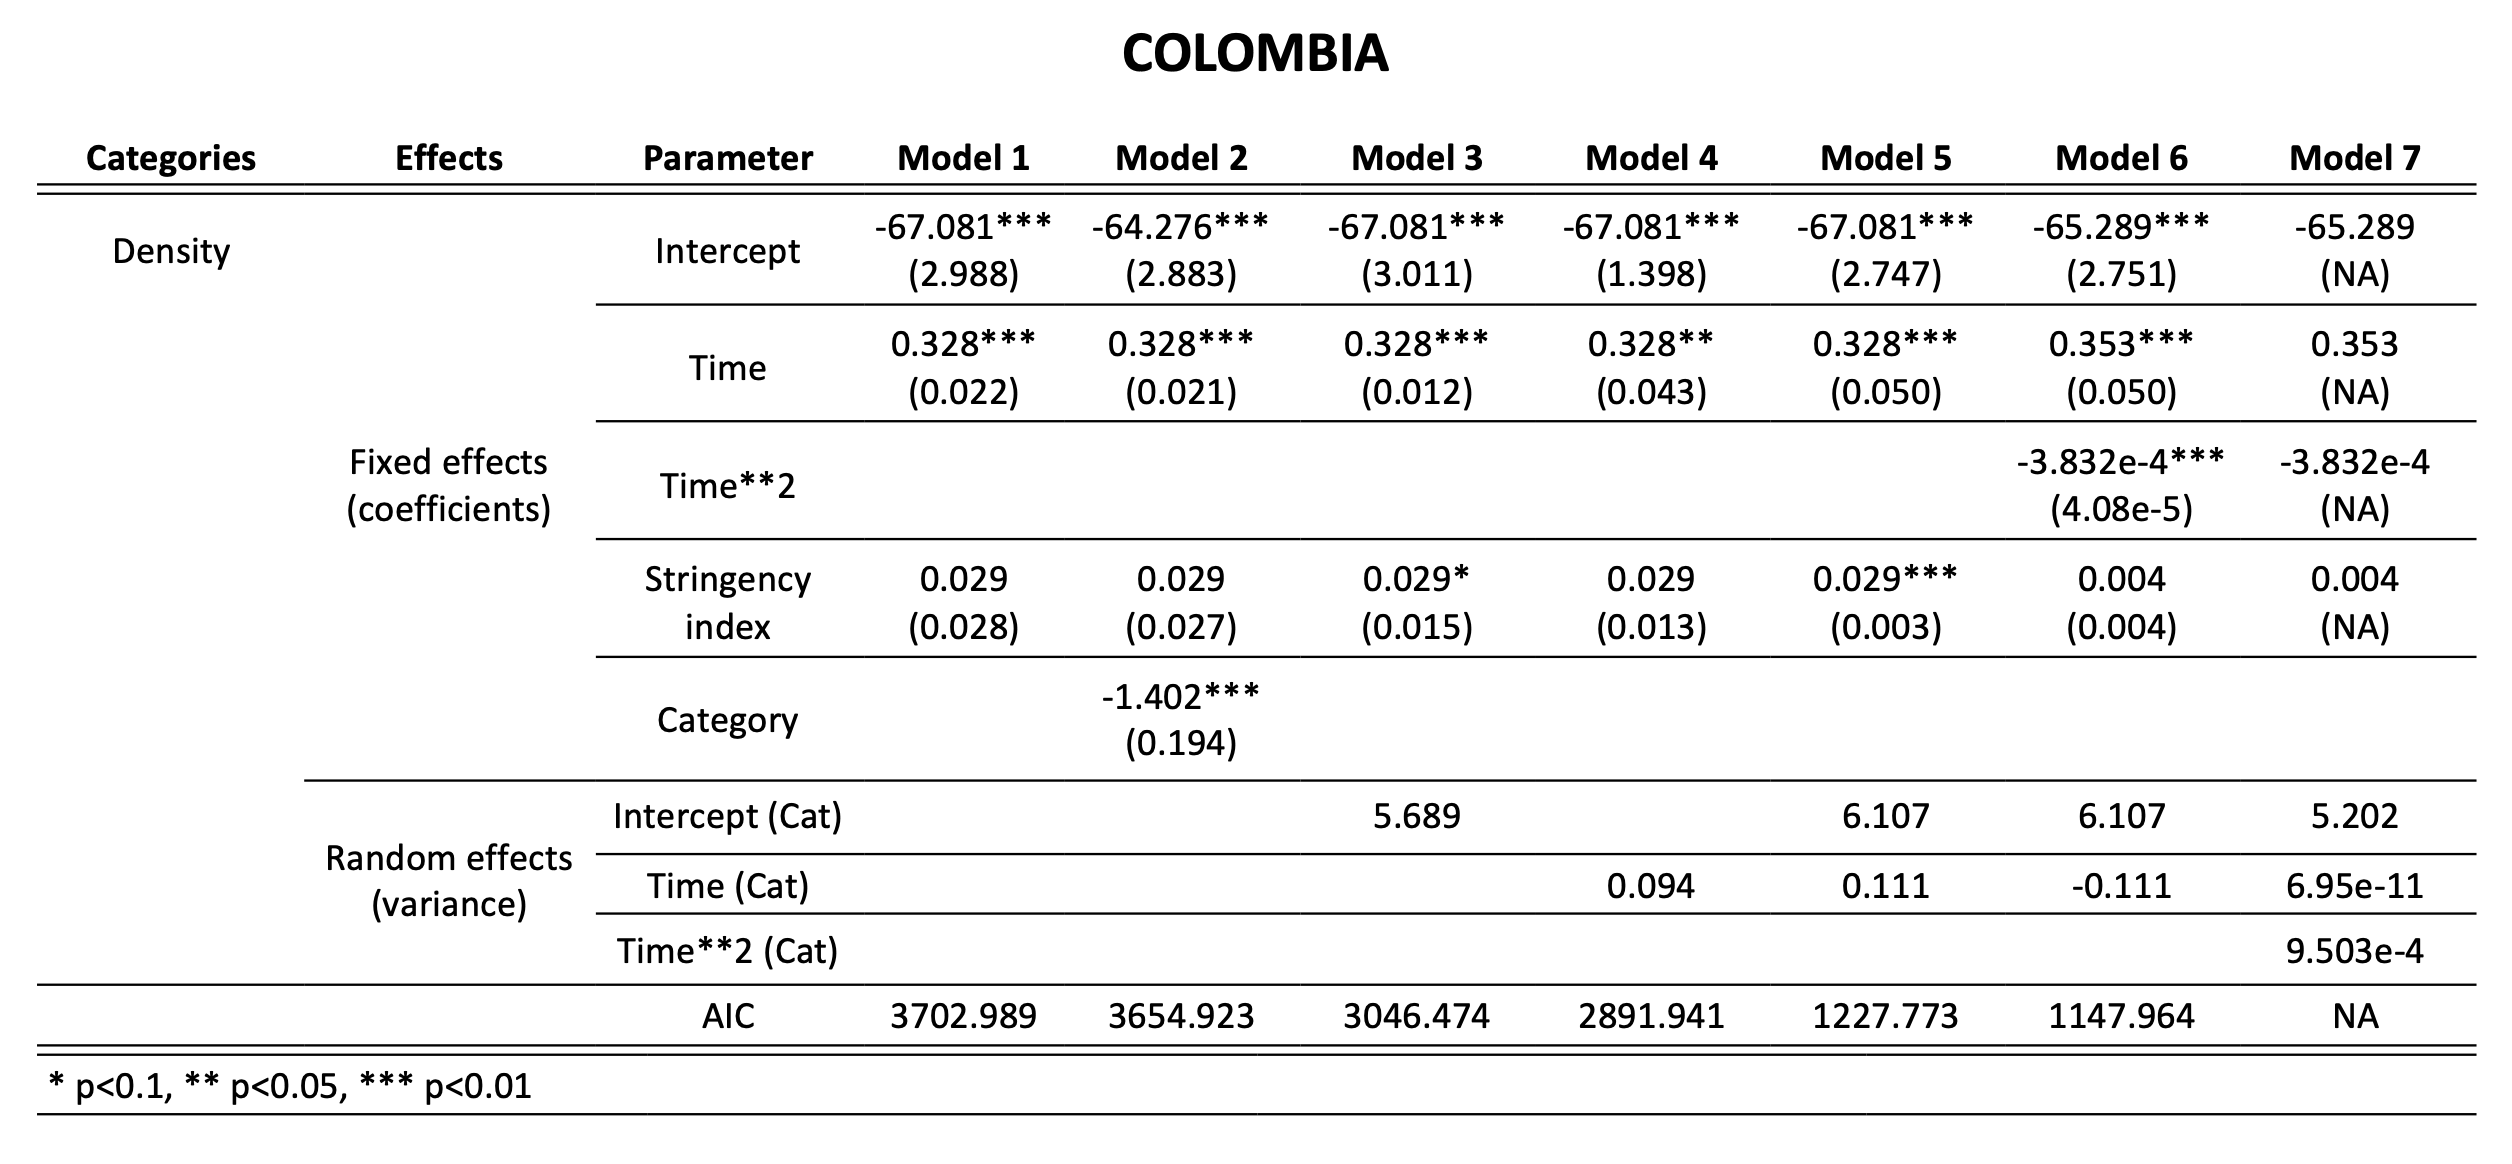
\includegraphics[width=\linewidth]{supplementary/models-tables/models-table-COL-quadratic-capital-stringency.png}
\caption{Results of mixed-effects models for trend analysis of relative change in netflows involving urban region surrounding capital in Colombia including stringency index as a predictor variable. Netflows are defined as inflows to an urban core minus outflows from the urban core. Random effects according to the population density or the Relative Deprivation Index (RDI) of the origin location of outflows.}
\label{tab-modelsCOL-capital-stringency}
\end{table}

\newpage

\subsection{Relative change in netflows involving all urban regions}

\begin{table}[h!]
\centering
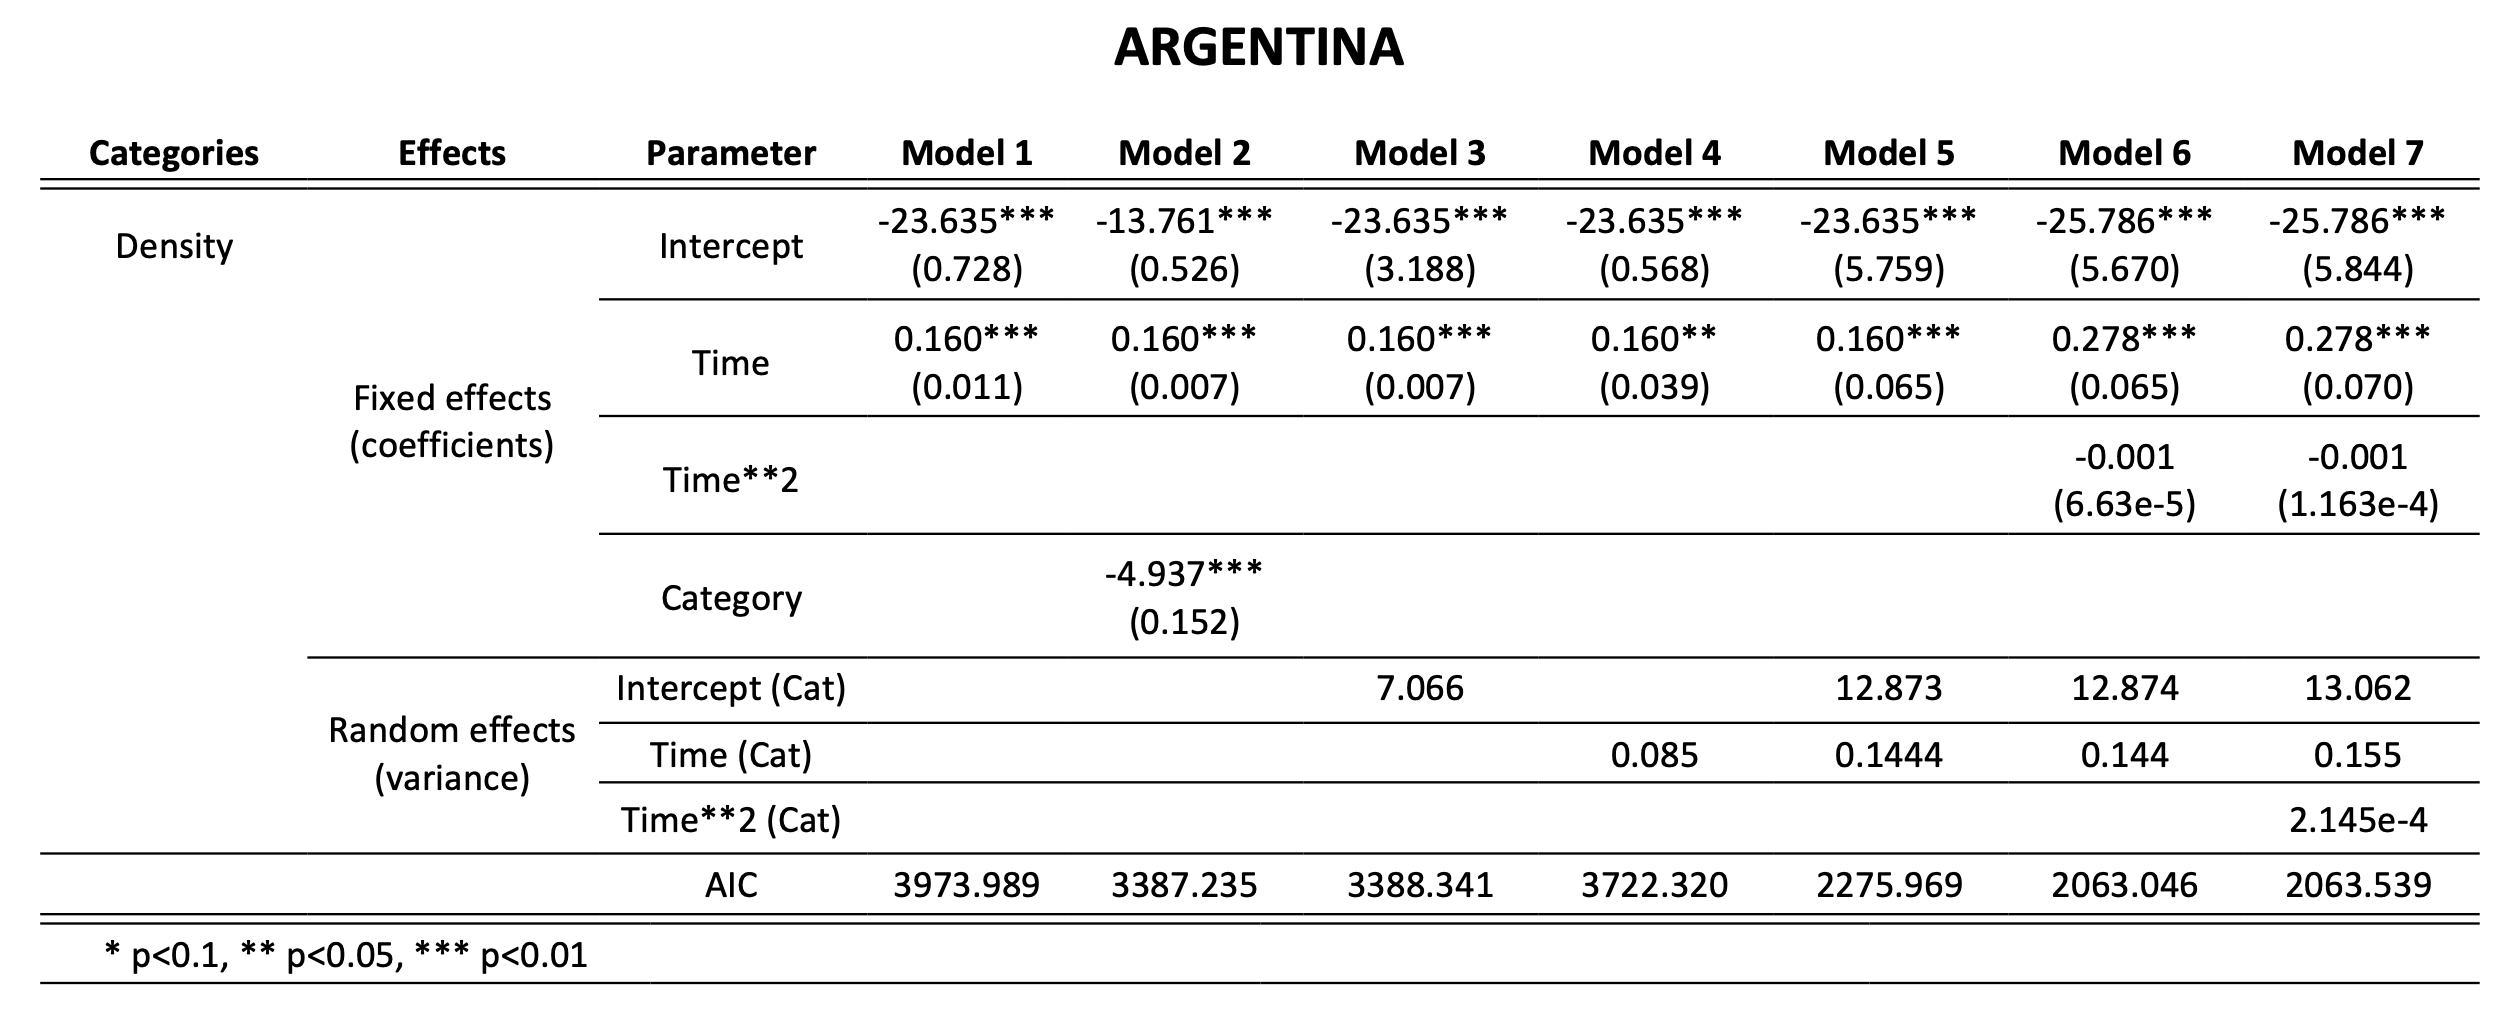
\includegraphics[width=\linewidth]{supplementary/models-tables/models-table-ARG-quadratic-fuas.png}
\caption{Results of mixed-effects models for trend analysis of relative change in netflows involving all urban regions in Argentina. Netflows are defined as inflows to an urban core minus outflows from the urban core. Random effects according to the population density or the Relative Deprivation Index (RDI) of the origin location of outflows.}
\label{tab-modelsARG-fuas}
\end{table}

\begin{table}[h!]
\centering
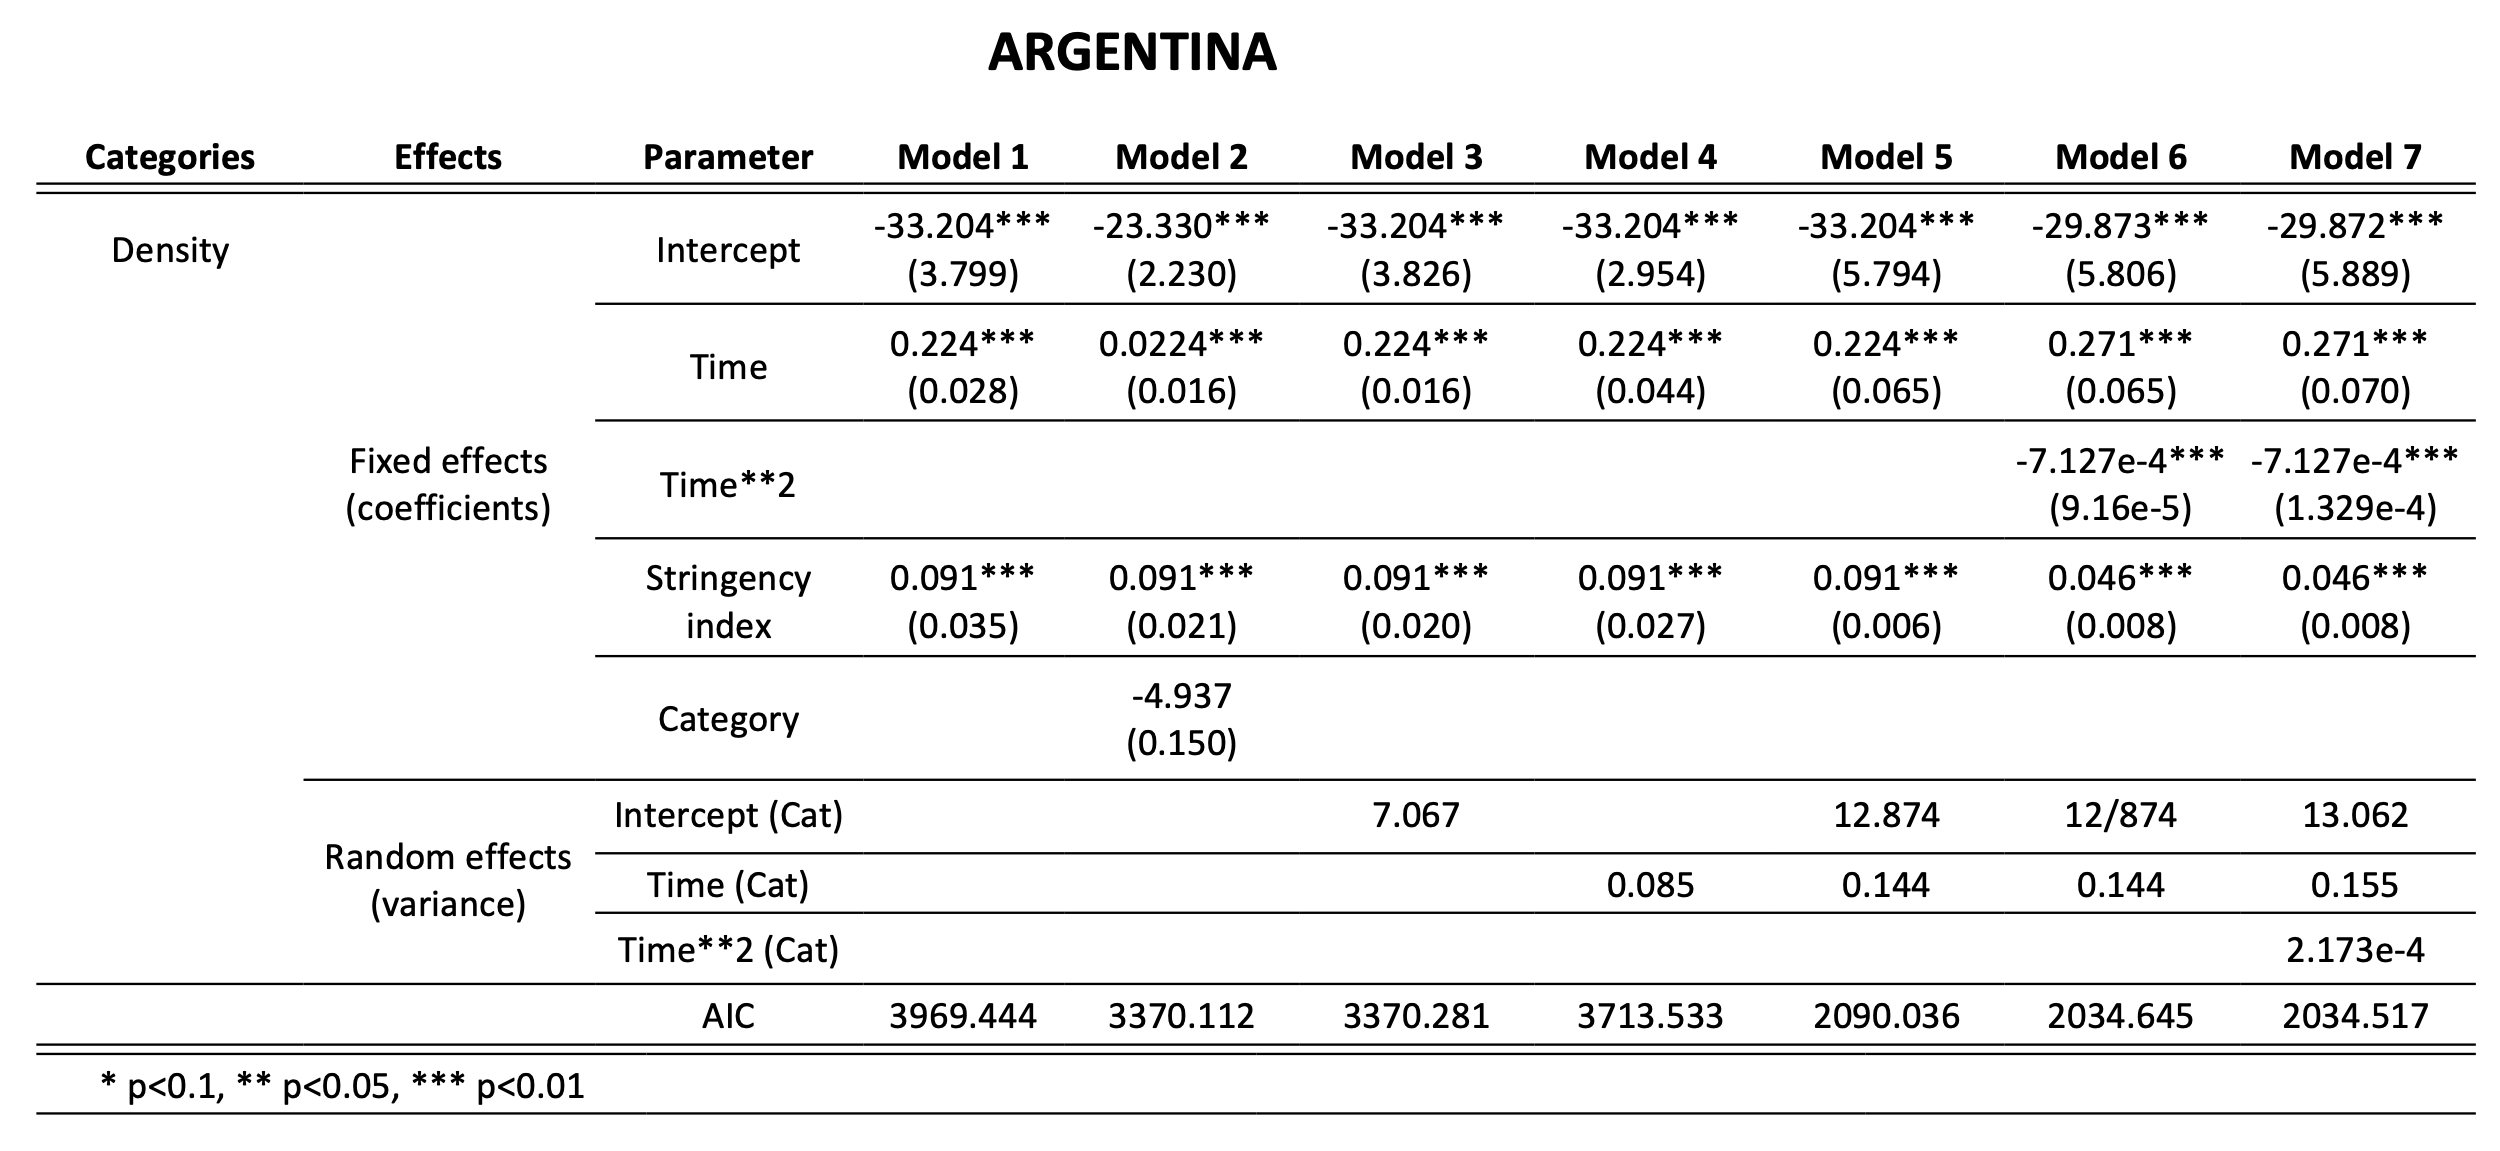
\includegraphics[width=\linewidth]{supplementary/models-tables/models-table-ARG-quadratic-fuas-stringency.png}
\caption{Results of mixed-effects models for trend analysis of relative change in netflows involving all urban regions in Argentina including stringency index as a predictor variable. Netflows are defined as inflows to an urban core minus outflows from the urban core. Random effects according to the population density or the Relative Deprivation Index (RDI) of the origin location of outflows.}
\label{tab-modelsARG-fuas-stringency}
\end{table}

\newpage

\begin{table}[h!]
\centering
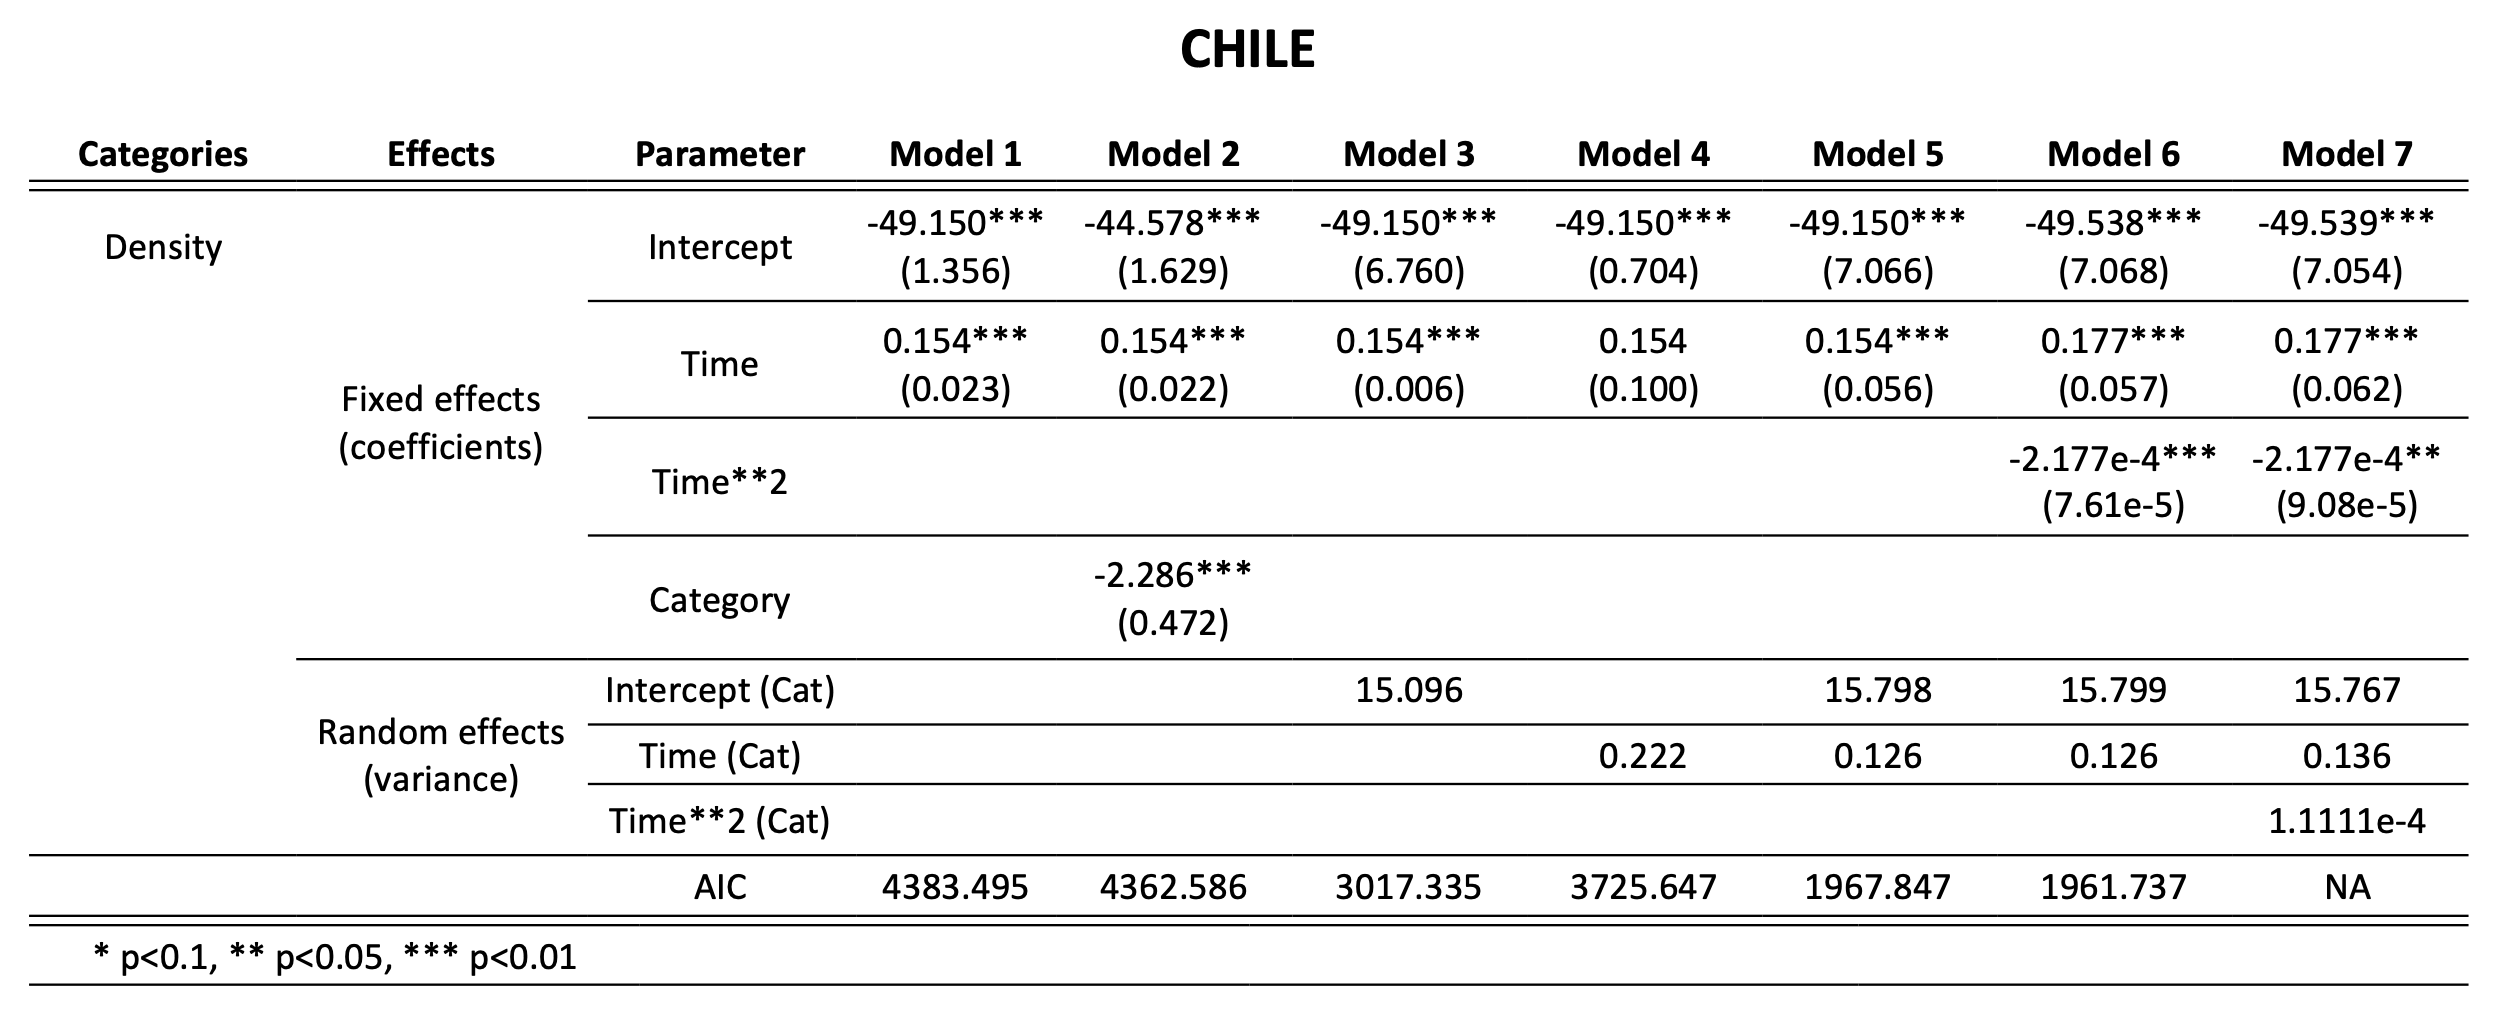
\includegraphics[width=\linewidth]{supplementary/models-tables/models-table-CHL-quadratic-fuas.png}
\caption{Results of mixed-effects models for trend analysis of relative change in netflows involving all urban regions in Chile. Netflows are defined as inflows to an urban core minus outflows from the urban core. Random effects according to the population density or the Relative Deprivation Index (RDI) of the origin location of outflows.}
\label{tab-modelsCHL-fuas}
\end{table}

\begin{table}[h!]
\centering
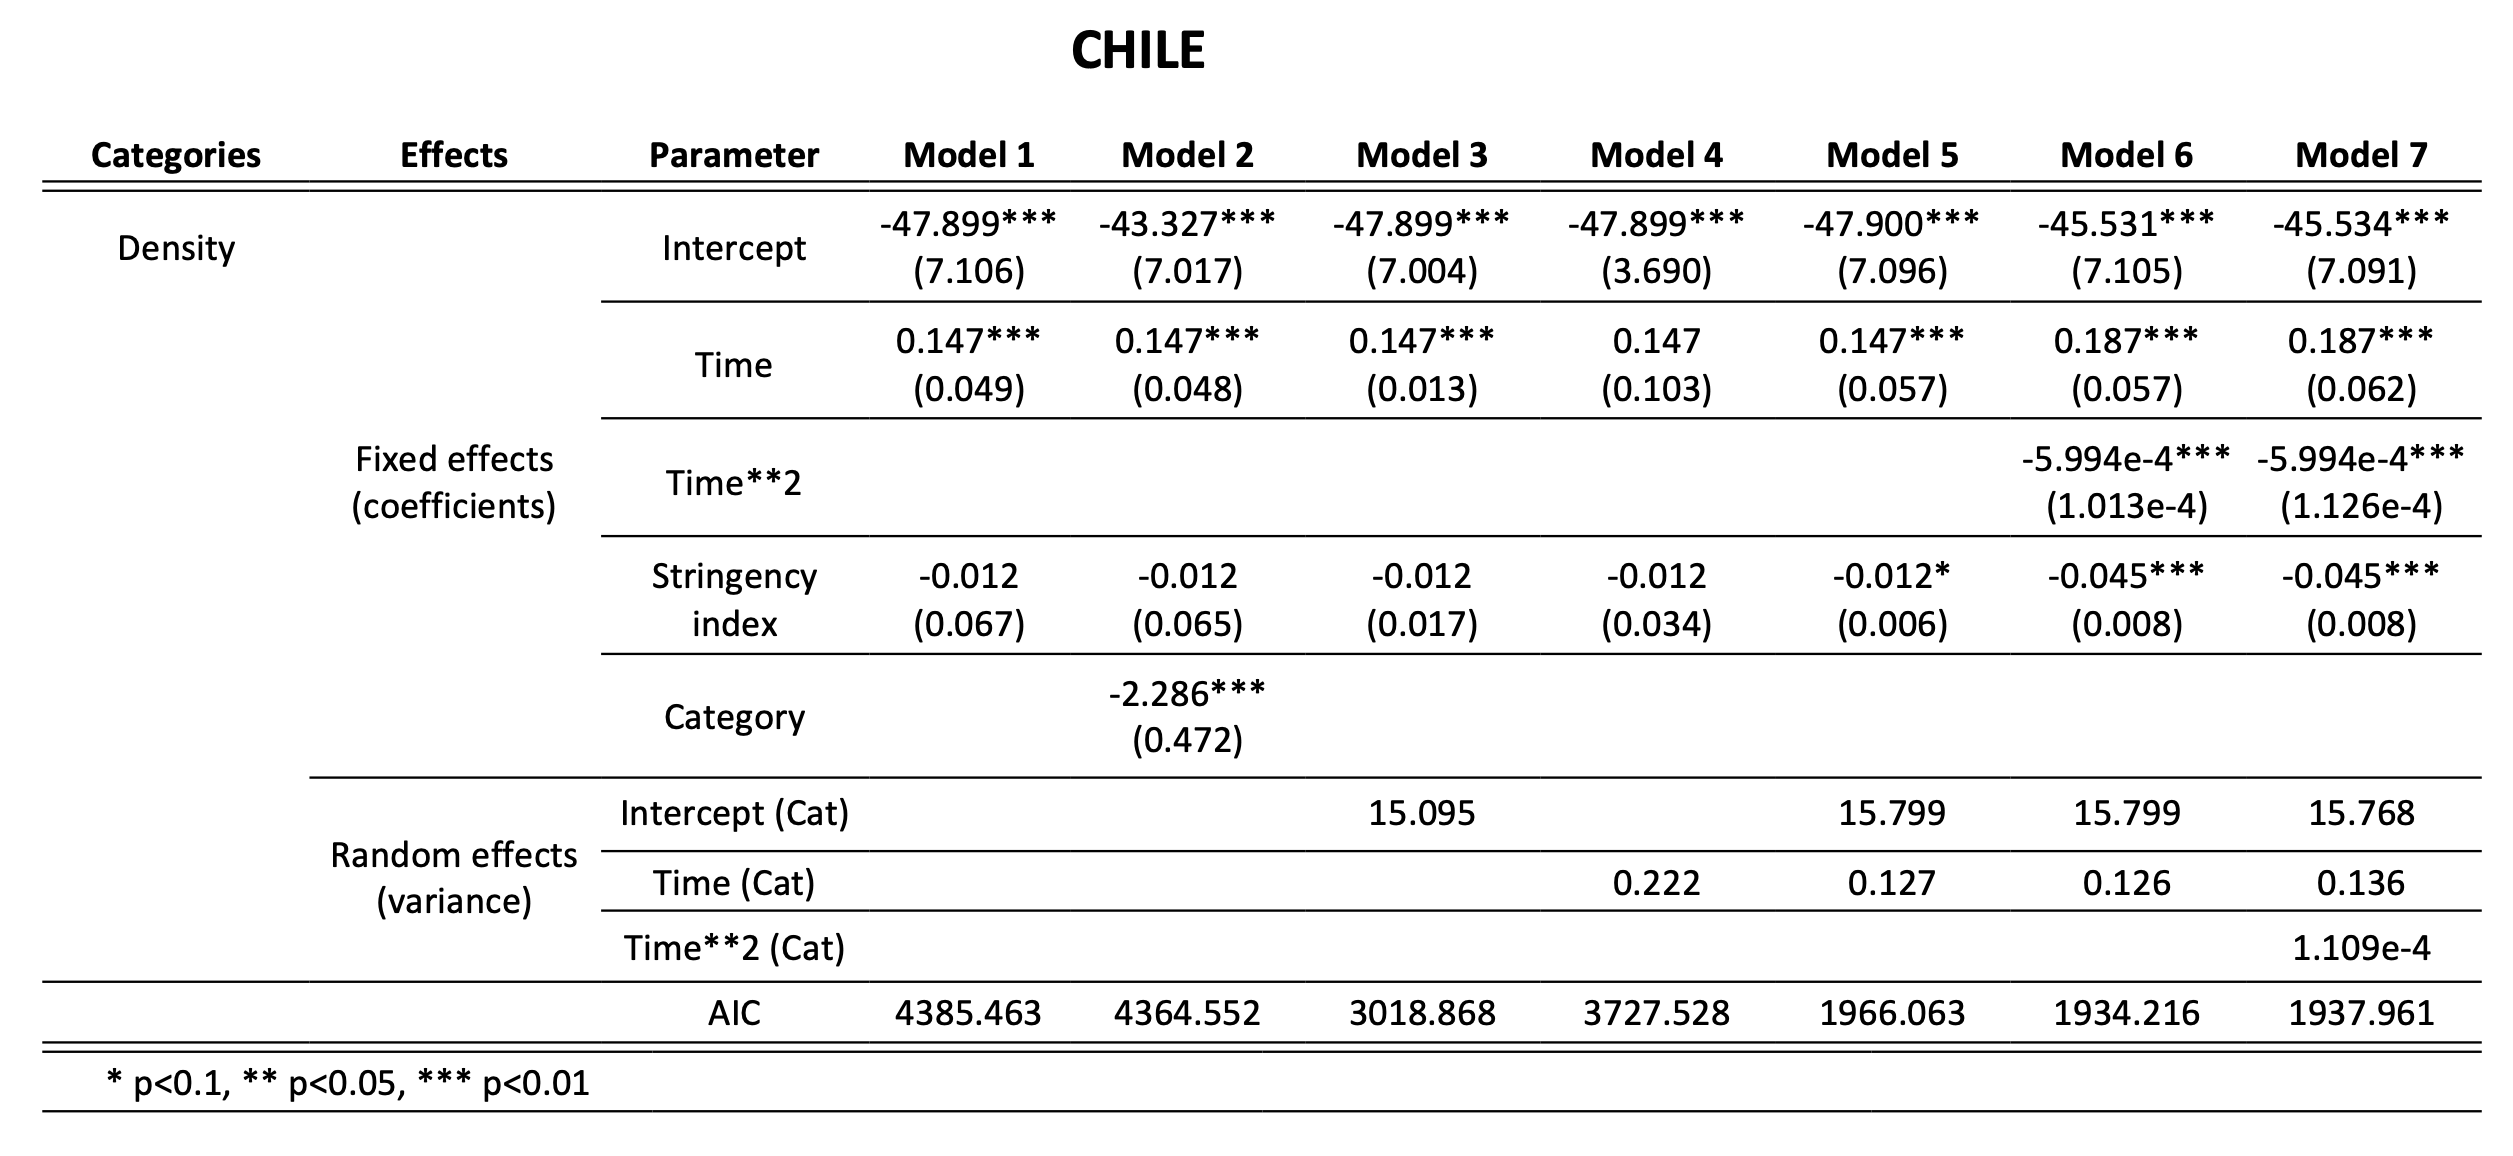
\includegraphics[width=\linewidth]{supplementary/models-tables/models-table-CHL-quadratic-fuas-stringency.png}
\caption{Results of mixed-effects models for trend analysis of relative change in netflows involving all urban regions in Chile including stringency index as a predictor variable. Netflows are defined as inflows to an urban core minus outflows from the urban core. Random effects according to the population density or the Relative Deprivation Index (RDI) of the origin location of outflows.}
\label{tab-modelsCHL-fuas-stringency}
\end{table}

\newpage

\begin{table}[h!]
\centering
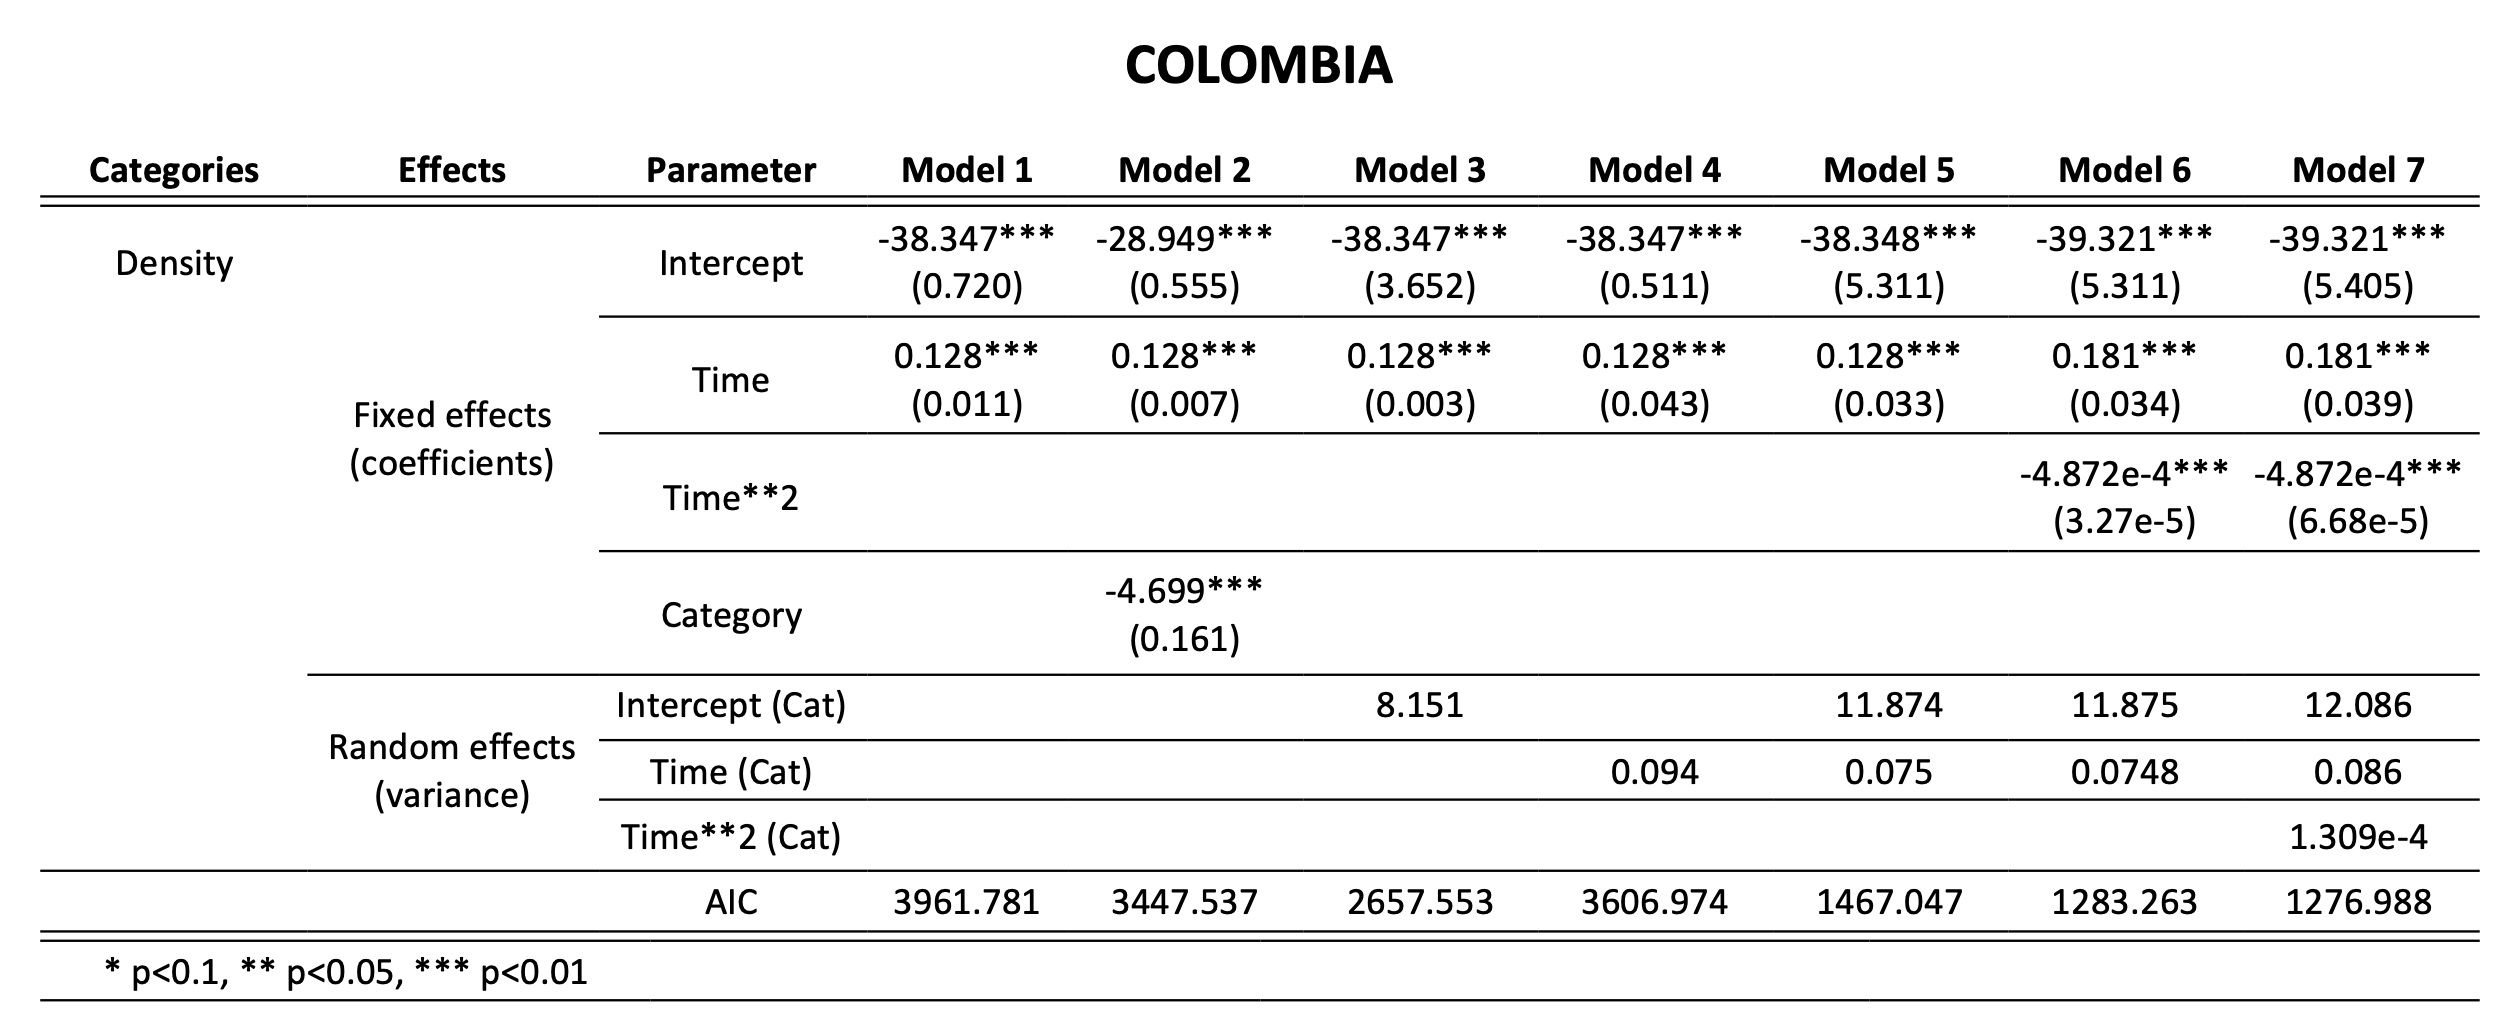
\includegraphics[width=\linewidth]{supplementary/models-tables/models-table-COL-quadratic-fuas.png}
\caption{Results of mixed-effects models for trend analysis of relative change in netflows involving all urban regions in Colombia. Netflows are defined as inflows to an urban core minus outflows from the urban core. Random effects according to the population density or the Relative Deprivation Index (RDI) of the origin location of outflows.}
\label{tab-modelsCOL-fuas}
\end{table}

\begin{table}[h!]
\centering
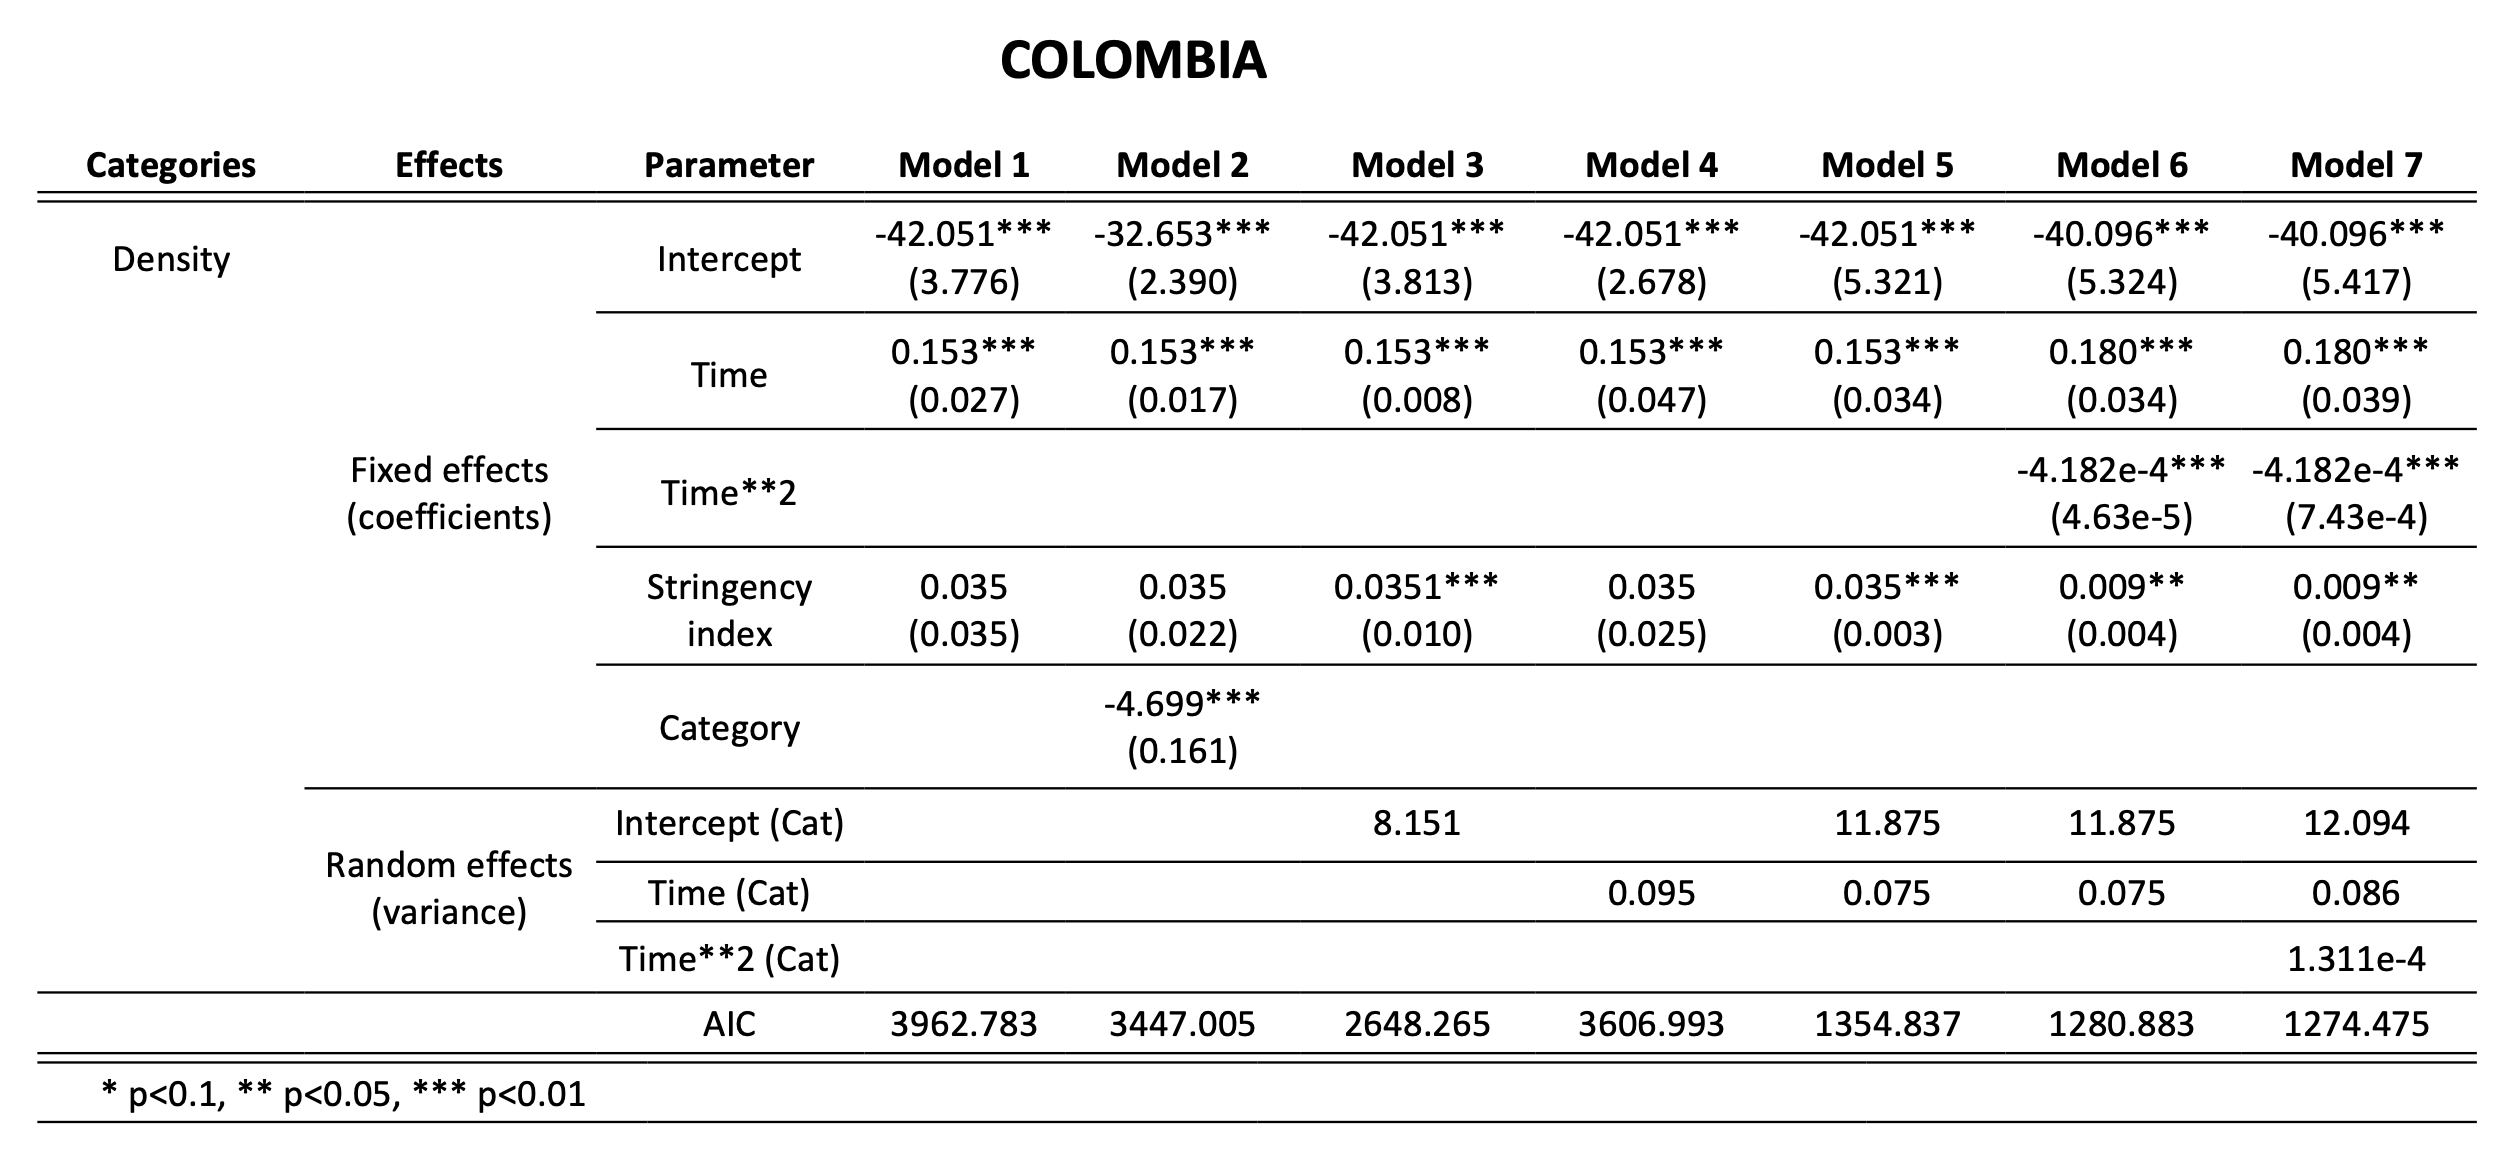
\includegraphics[width=\linewidth]{supplementary/models-tables/models-table-COL-quadratic-fuas-stringency.png}
\caption{Results of mixed-effects models for trend analysis of relative change in netflows involving all urban regions in Colombia including stringency index as a predictor variable. Netflows are defined as inflows to an urban core minus outflows from the urban core. Random effects according to the population density or the Relative Deprivation Index (RDI) of the origin location of outflows.}
\label{tab-modelsCOL-fuas-stringency}
\end{table}

\newpage

\section{Recovery times}

\subsection{Deriving recovery time formula (equation 7)}

We begin by assuming a quadratic model to describe the evolution of mobility levels over time relative to the baseline:
\begin{equation}
    y(t) = a + b\cdot t + c\cdot t^2
\end{equation}\label{model-trend}

The coefficients \( a \), \( b \), and \( c \) can be expressed in terms of the parameters from equation (6) in the main text. For instance, under Model 6, we have \( a = \beta_0 + b_0 \), \( b = \beta_1 + b_{1i} \), and \( c = \beta_2 \).

The recovery time to a threshold \( \alpha \), denoted by \( t_{\alpha} \), is defined as the time it takes for \( y(t) \) to recover by \( \alpha\% \). If the mobility level relative to the baseline at time \( t = 0 \) is \( a \), then \( t_{\alpha} \) is the time at which
\[
y(t_{\alpha}) = \left(1 - \frac{\alpha}{100}\right) a.
\]

Substituting this into equation \eqref{model-trend} and solving for \( t_{\alpha} \), we obtain:
\begin{equation}
    t_{\alpha} = \frac{-b \pm \sqrt{b^2 - 4c \left( \frac{\alpha}{100} \right) a}}{2c}
\end{equation}\label{recovery-time}

A recovery time is only meaningful if mobility initially decreased relative to the baseline, which imposes the condition \( a < 0 \). Moreover, since we are referring to a ``recovery,'' the trend must be increasing at \( t = 0 \), requiring \( y'(0) > 0 \), or equivalently, \( b > 0 \). As we are only interested in positive time values, and given \( b > 0 \), we select the solution with the \( + \) sign in equation \eqref{recovery-time}.

Finally, if \( b^2 - 4c \left( \frac{\alpha}{100} \right) a < 0 \), there is no real-valued solution for \( t_{\alpha} \). In such cases, we interpret this as mobility levels never reaching the specified recovery threshold.

The recovery time can also be obtained under a linear model (e.g. Model 5). The derivation is then analogous, but $y(t) = a + b\cdot t$ and therefore, $t_\alpha$ is given by:
\begin{equation}
    t_{\alpha} = -\dfrac{\alpha}{100}\cdot \dfrac{a}{b}
\end{equation}

\subsection{Computation of uncertainty for recovery times}

According to Model 6, the recovery time at threshold $\alpha$ is given by equation \eqref{recovery-time} where $a$, $b$ and $c$ are the coefficients for the intercept, linear and quadratic terms in equation \eqref{model-trend}.

The partial derivatives are:
\[
\frac{\partial t_\alpha}{\partial a} = \frac{-\frac{\alpha}{100}}{\sqrt{b^2 - 4c\frac{\alpha}{100} a}}, \quad
\frac{\partial t_\alpha}{\partial b} = \frac{1}{2c} \left( -1 + \frac{b}{\sqrt{b^2 - 4c\frac{\alpha}{100} a}} \right), \quad
\frac{\partial t_\alpha}{\partial c} = \frac{(b - \sqrt{b^2 - 4c\frac{\alpha}{100} a})\sqrt{b^2 - 4c\frac{\alpha}{100} a} - 2\frac{\alpha}{100} a c}{2c^2\sqrt{b^2 - 4c\frac{\alpha}{100} a}}
\]

The propagated uncertainty is:
\[
\sigma_t = \sqrt{
\left( \frac{\partial t_\alpha}{\partial a} \right)^2 \sigma_a^2 +
\left( \frac{\partial t_\alpha}{\partial b} \right)^2 \sigma_b^2 +
\left( \frac{\partial t_\alpha}{\partial c} \right)^2 \sigma_c^2}
\]

If using a linear model to estimate $t_{\alpha}$, like Model 5, then:
\[
\frac{\partial t_\alpha}{\partial a} = -\frac{\alpha}{100} \cdot \frac{1}{b}, \quad
\frac{\partial t_\alpha}{\partial b} = \dfrac{\alpha}{100}\cdot\dfrac{a}{b^2}
\]
and the propagated uncertainty is 
\begin{displaymath}
    \sigma_{t_\alpha} = \sqrt{
\left( \frac{\partial t_\alpha}{\partial a} \right)^2 \sigma_a^2 +
\left( \frac{\partial t_\alpha}{\partial b} \right)^2 \sigma_b^2 }
\end{displaymath}

\newpage

\subsection{Estimated recovery times}

\begin{table}[h!]
\centering
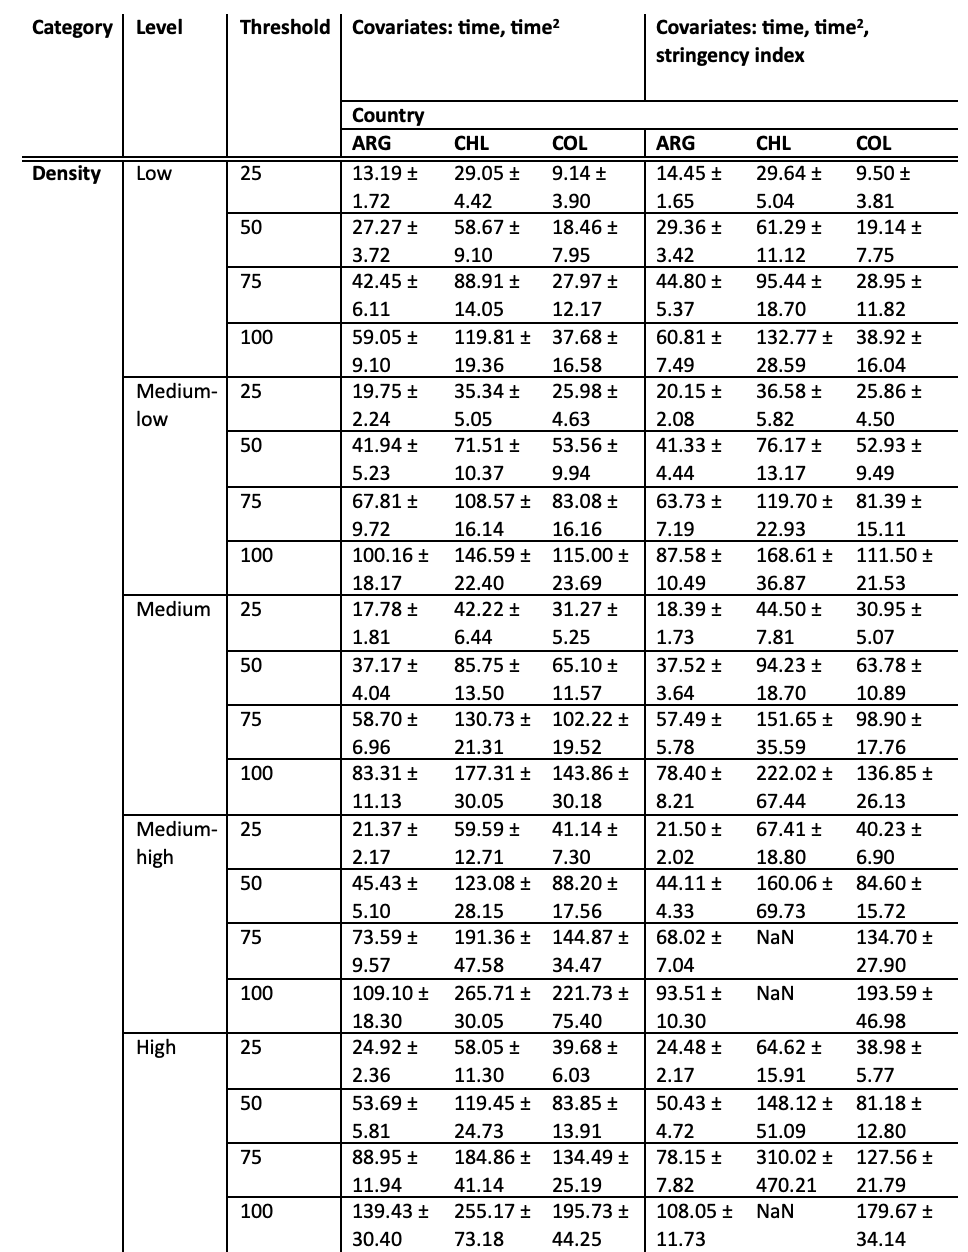
\includegraphics[width=0.9\linewidth]{supplementary/recovery-times/recovery-thresholds-table-quadratic-std-density.png}
\caption{Recovery times at multiple thresholds, for outflows in Argentina, Chile and Colombia, by population density . Computed using Model 6, with covariates time and time$^2$, or time, time$^2$ and stringency index. N/A values correspond to cases where the initial mobility levels are above the baseline. NaN values correspond to cases where mobility never recovers to the specified threshold.}
\end{table}

\begin{table}[h!]
\centering
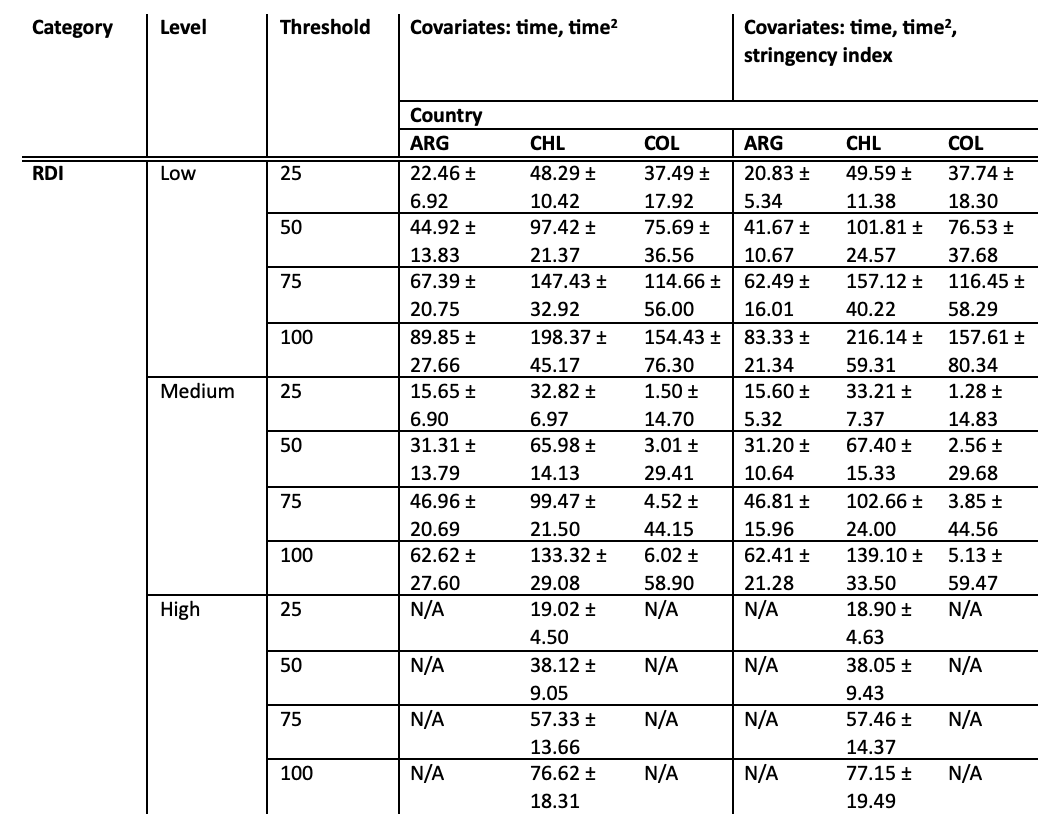
\includegraphics[width=0.9\linewidth]{supplementary/recovery-times/recovery-thresholds-table-quadratic-std-rdi.png}
\caption{Recovery times at multiple thresholds, for outflows in Argentina, Chile and Colombia, by Relative Deprivation Index (RDI) category. Computed using Model 6, with covariates time and time$^2$, or time, time$^2$ and stringency index. N/A values correspond to cases where the initial mobility levels are above the baseline. NaN values correspond to cases where mobility never recovers to the specified threshold.}
\end{table}

\begin{table}[h!]
\centering
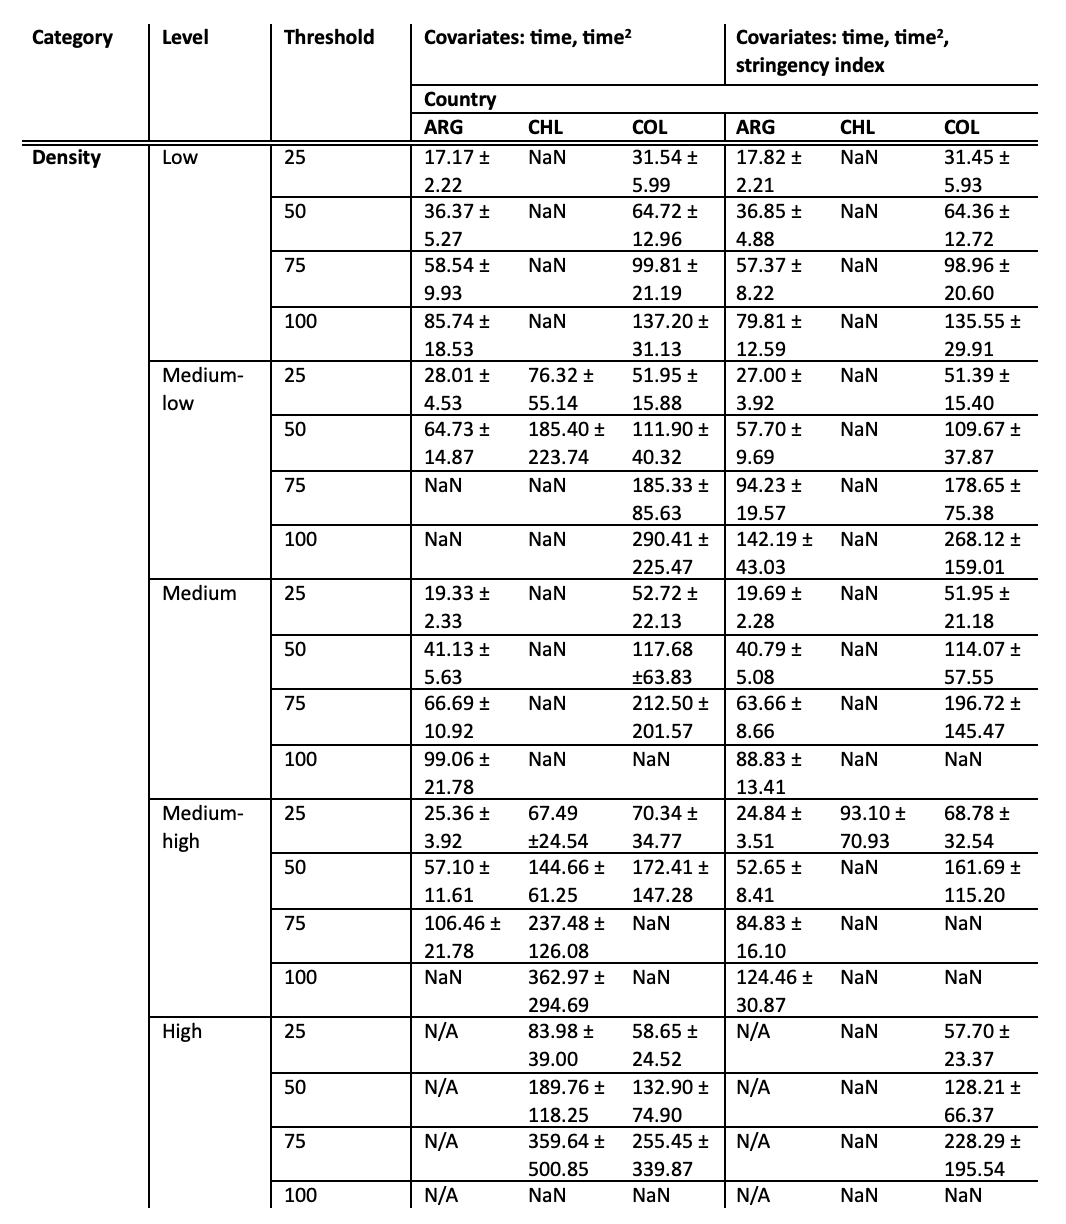
\includegraphics[width=0.9\linewidth]{supplementary/recovery-times/recovery-thresholds-table-quadratic-capital-std.png}
\caption{Recovery times at multiple thresholds, for netflows involving the urban region surrounding the capital in Argentina, Chile and Colombia, by population density category. Computed using Model 6, with covariates time and time$^2$, or time, time$^2$ and stringency index. N/A values correspond to cases where the initial mobility levels are above the baseline or the only cell in a population density category is the centre of netflows. NaN values correspond to cases where mobility never recovers to the specified threshold.}
\label{tab-rec-times-capital}
\end{table}

\begin{table}[h!]
\centering
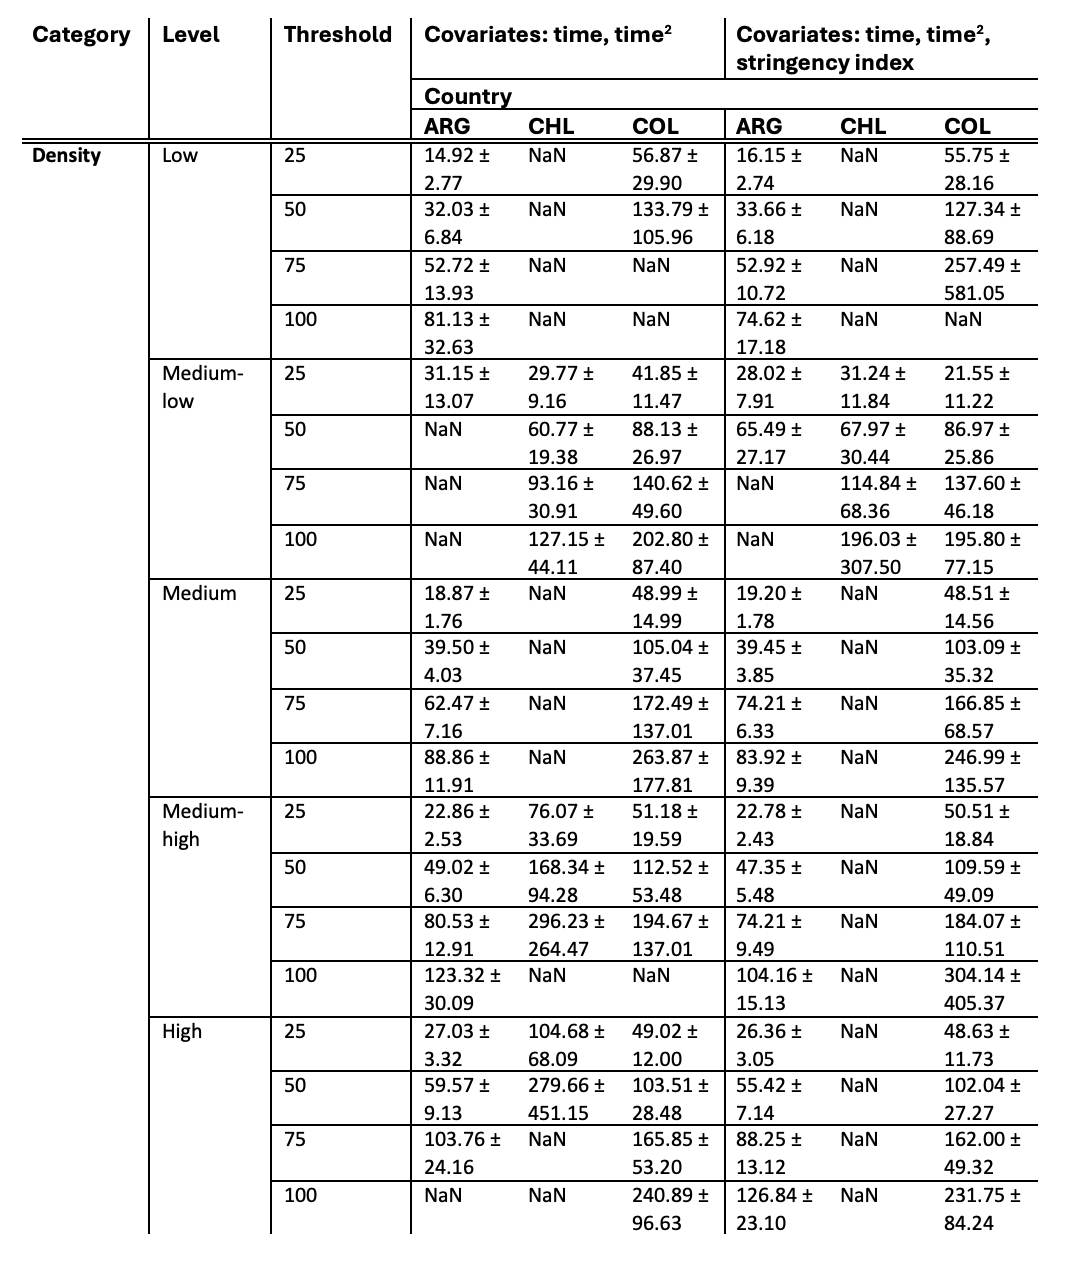
\includegraphics[width=0.9\linewidth]{supplementary/recovery-times/recovery-thresholds-table-quadratic-fuas-std.png}
\caption{Recovery times at multiple thresholds, for netflows involving all urban regions in Argentina, Chile and Colombia, by population density category. Computed using Model 6, with covariates time and time$^2$, or time, time$^2$ and stringency index. NaN values correspond to cases where mobility never recovers to the specified threshold.}
\label{tab-rec-times-fuas}
\end{table}

\end{document}